%appendixprefix sorgt daf�r, dass "Anhang" vor jedem Anhang steht
%openany sorgt daf�r, dass ein Kapitel auf jeder Seite beginnen kann
%        nicht nur rechts
%bibtotoc sorgt daf�r, dass das Literaturverzeichnis automatisch im
%         Inhaltsverzeichnis erscheint
%\documentclass[colordvi,11pt,a4paper,halfparskip,final,headings,appendixprefix,bibtotoc]{scrbook}
\documentclass[
  pdftex,
  chapterprefix,
  headsepline,
  footsepline,
  colordvi,
  11pt,
  a4paper,
  halfparskip,
  final,
  appendixprefix,
  bibtotoc]{scrbook}
% uncomment the following line (mutual exclusive to the one above) to enter the draft mode.
%\documentclass[colordvi,11pt,a4paper,halfparskip,draft,appendixprefix,bibtotoc]{scrbook}


%
% neues if definieren, um zwischen PDF und DVI entscheiden zu k�nnen.
%
\usepackage{ifpdf}
\ifx\pdfoutput\undefined
\pdffalse %not PDFLaTeX
\else
\pdfoutput=1
\pdftrue
\fi
%\tracingstats=2
%\usepackage{layout}
% german language support (hyphenation etc)  
\usepackage[ngerman]{babel}

% for prettier tables
\usepackage{booktabs}

% support for latin1 characters. That means you can enter umlauts directly
% no need for "a "u "o "s anymore
\usepackage[utf8x]{inputenc}
%\usepackage[latin1]{inputenc}

% provides the \url{} command to pretty print urls
\usepackage{url}

% provides code
\usepackage{listings}
\lstset{
	language=Python,
	basicstyle=\ttfamily
}

% needed for a german bibliography-style (s. below)
\usepackage{bibgerm}

% allows text flowing around figures.
\usepackage{wrapfig}

% allows to \includegraphics
\usepackage{graphicx}

% defines some standard colornames like "black" etc.
\usepackage{color}

% allows to color tablecells
\usepackage{colortbl}

% provides an easier interface to if-then-else constructs in 
% custom macros
\usepackage{ifthen}

% allows tables to break over pages.
\usepackage{supertabular}

% allows to have different kinds paper orientations in the same pdf-documnent
\usepackage{pdflscape}

% allows to specify absolute texpos for textboxes. This is generally only important for the titlepage
\usepackage[absolute]{textpos}

% allows to enumerate different figures with a) b) in the same figure-environment.
\usepackage{subfigure}

% finetune the gaps between figure and text in the subfigure environment (basically close the gap as much as possible)
\renewcommand{\subfigtopskip}{0pt}
\renewcommand{\subfigbottomskip}{0pt}

% some color definitions for the pdf statements below
\definecolor{mygrey}{rgb}{0.45,0.45,0.45}
\definecolor{mydarkgrey}{rgb}{0.2,0.2,0.2}
\definecolor{red}{rgb}{1.0,0.33,0.33}
\definecolor{orange}{rgb}{1.00,0.73,0.33}
\definecolor{yellow}{rgb}{0.95,0.92,0.}
\definecolor{lightgreen}{rgb}{0.3,0.95,0.46}
\definecolor{titleblue}{rgb}{0.03,0.10,0.46}

\ifpdf
% Metadata and configuration of the pdf output:
% Do not forget to enter the correct title, author, subject und keywords

% For screen viewing it is nice to have references marked in a slightly different
% color than the rest of the text. Since they will be hyperlinks to the 
% referenced objects.
\usepackage[pdftex,
             pdftitle={},
             colorlinks,
             linkcolor={mydarkgrey},
             citecolor={mygrey},
             urlcolor={black},
             plainpages={false},
             bookmarksnumbered={true},
             pdfauthor={},
             pdfsubject={},
             pdfkeywords={},
             pdfstartview={FitBH}]{hyperref}

% For the final printouts (remember - you need at least three - one for each examiner and one for the archive 
% [ This might have changed - so contact the "Pr�fungsamt" about the current regulations !! ] - it is better
% to have all text in the same color (namely black).
% 
%\usepackage[pdftex,
%            pdftitle={},
%            colorlinks,
%            linkcolor={black},
%            citecolor={black},
%            urlcolor={black},
%            plainpages={false},
%            bookmarksnumbered={true},
%            pdfauthor={},
%            pdfsubject={},
%            pdfkeywords={},
%            pdfstartview={FitBH}]{hyperref}
\pdfcompresslevel=9
\fi

% some configuration for the amount of text on a single page
\usepackage{typearea}
\areaset[1.5cm]{418pt}{658pt}
\setlength{\headheight}{37pt}

% Enter author and title for the titlepage.
\author{}
\title{}

% To avoid nasty mistakes like having comments directly in the textflow
% the following \todo macro was defined. With that you can enter
% \todo{What I still have to do here} 
% inside of your text and a marker will appear at the page's margin with the 
% text "What I still have to do here".
% The first line activates this feature. If you comment it out and uncomment
% the second line below there will be no error messages and no todos will be shown
% anymore. So - even if you have forgotten to delete one of them - they will not appear
% in the final printout. 
\newcommand{\todo}[1]{\marginpar{\textcolor{red}{ToDo:} #1}}
%\newcommand{\todo}[1]{}

% We recommend to split your document into several files. Usually one for every chapter is a 
% good idea. If you follow this guideline (how to assemble these files in a single document
% see two paragraphs below) you will be able to single out chapters via the \includeonly{}
% command. Using this mechanism page numbering and references of the full run before will be
% preserved. This also nice, if your latex run tends to get slow and you need to fine tune 
% some formatting in one chapter - just include that one. The rest (or at least the ones before
% the one currently under construction) will remain untouched. This means a boost in compilation time.
%\includeonly{chapter2}

\begin{document}
% the next two lines influence the detailedness of the table of contents
% and to what structure depth numbers are written before sections/subsections/paragraphs
% You should not touch this
\setcounter{tocdepth}{2}
\setcounter{secnumdepth}{3}
\frontmatter
% here the titlepage is included. Look into the file "titlePage.tex" to 
% adapt it to your needs (name, title etc.)
%!TEX root=../../Vorname_Nachname_Diplomarbeit.tex

% Titelseite braucht folgenden  Eintrag
% \usepackage[absolute]{textpos}
% textpos ist nicht Bestandteil von tetex
% kann aber von dante heruntergeladen werden
\begin{titlepage}
\vspace*{-1cm}
\newlength{\links}
\setlength{\links}{0.9cm}
\setlength{\TPHorizModule}{1cm}
\setlength{\TPVertModule}{1cm}
\textblockorigin{0pt}{0pt}

\sf
\LARGE

\begin{textblock}{16.5}(2.8,2.6)
 \hspace*{-0.25cm} \textbf{UNIVERSITÄT DUISBURG-ESSEN} \\
 \hspace*{-1.15cm} \rule{5mm}{5mm} \hspace*{0.05cm} FAKULTÄT FÜR INGENIEURWISSENSCHAFTEN\\
 \large{}ABTEILUNG INFORMATIK UND ANGEWANDTE KOGNITIONSWISSENSCHAFT\\
\end{textblock}


%Hier Titel, Name, und Matrikelnummer eintragen, \\ make a newline
\begin{textblock}{14.5}(3.2,8.5)
  \large
{ \bf Bachelorarbeit} \\[1cm]
{\LARGE \Large\bf Untersuchung der Auswirkungen von Quantisierung und Pruning auf Convolutional Neural Networks für Mobilgeräte} \\[1.3cm]
Julian Hoever\\
Matrikelnummer: 3075732\\
Studiengang: Angewandte Informatik
\end{textblock}



\begin{textblock}{10}(10.5,17.5)

\includegraphics[scale=1.0]{content/images/unilogo.pdf}\\
\normalsize
\raggedleft
Eingebettete Systeme der Informatik, Abteilung Informatik \\
Fakultät für Ingenieurwissenschaften \\
Universität Duisburg-Essen \\[2ex]

\today\\[15ex]
\raggedright
% Supervisors
{\bf Erstgutachter:} Prof. Dr. Gregor Schiele \\
{\bf Zweitgutachter:} Prof. Dr. Torben Weis \\
{\bf Zeitraum:} 15.Dezember 2020 - 16.März 2021\\
\end{textblock}

\end{titlepage}

%\setcounter{page}{2}

\cleardoublepage



\section*{Kurzfassung}
Modelle des maschinellen Lernens wurden in den letzten Jahren zum Lösen von immer mehr Problemen eingesetzt. Besonders neuronale Netzwerke spielen dabei eine zunehmend wichtige Rolle. Um diese neuronalen Netze, welche meist sehr groß und ressourcenintensiv sind, auf eingebetteten und mobilen Plattformen einsetzen zu können, sind spezielle, für diesen Anwendungsbereich, optimierte Netzwerkarchitekturen notwendig. Die Netzwerkarchitekturen für mobile und eingebettete Systeme wenden dazu häufig architekturelle Veränderungen an, wie zum Beispiel den Einsatz von Depthwise Separable Convolutions oder der Einsatz von Squeeze-And-Excitation Modulen, um eine gesteigerte Effizienz zu erreichen.

Diese Arbeit stellt dazu eine Auswahl an Netzwerkarchitekturen vor, die für den Anwendungsbereich der Bildverarbeitung auf mobilen und eingebetteten Systeme geeignet sind. Dabei handelt es sich im Wesentlichen um die Architekturen MobileNet, MobileNetV2, MobileNetV3 Large/Small und EfficientNet. Die vorgestellten Architekturen werden auf dem CIFAR-10 Datensatz trainiert und miteinander verglichen. Außerdem werden in dieser Arbeit die Optimierungstechniken Quantisierung und Pruning vorgestellt und systematisch auf die Netzwerkarchitekturen angewendet. Es soll ermittelt werden wie sich diese Architekturen und die architekturellen Optimierungen unter Anwendung von Quantisierung und Pruning verhalten. Für das Pruning der Architekturen wird in dieser Arbeit ein einfaches Magnitude Pruning verwendet und für die Quantisierung wird eine Post-Training Quantisierung angewendet. Die resultierenden Modelle werden für die Evaluation auf einem Raspberry Pi 4 ausgewertet.

Im Verlauf der Evaluation hat sich herausgestellt, dass sich der Speicherbedarf der Modelle, allein durch die Anwendung von Quantisierung, deutlich reduzieren lässt und das teilweise ohne einen Verlust an Genauigkeit. Zusätzlich ist es durch eine Kombination aus Pruning und einem Kompressionsalgorithmus wie gzip möglich, Modelle sehr stark zu komprimieren. Die kleinsten Modelle konnten in dieser Arbeit durch eine Kombination aus Pruning, Quantisierung und der Anwendung von gzip erreicht werden. Durch die Anwendung dieser Kombination konnte der Hintergrundspeicherbedarf der Modelle im Durchschnitt bis zu 91.65\% verringert werden. Um die Auswirkungen der Optimierungstechniken Quantisierung und Pruning zu untersuchen wurde als weitere Metrik die klassenweise Genauigkeit \cite{hooker_what_2020} vorgestellt und exemplarisch an der MobileNet und EfficientNet-B0 Architektur evaluiert. Dabei wurde gezeigt, dass sich der Verlust durch Pruning und Quantisierung ungleichmäßig auf die einzelnen Klassen auswirkt und somit unbedingt beachtet werden sollte, um die Qualität eines geprunten oder quantisierten Modells zu bewerten. Als letztes wurden anhand der MobileNetV3 Minimalistic Architekturen mögliche architekturelle Optimierungen betrachtet, um die vorgestellten Netzwerkarchitekturen bezüglich der Inferenzzeit und der Quantisierbarkeit zu optimieren.



\cleardoublepage

\tableofcontents

%\listoffigures
\mainmatter

% To assemble the whole document
% Please be aware that each file will begin on a new page
% therefore chapters should be put into such a file.
% There cannot be an include statement inside of an "included" file.
% So if you want to further divide your document - use \input inside of 
% the included files. \input will not begin on a new page.
\chapter{Einleitung}
In diesem einleitenden Kapitel wird im ersten Abschnitt das Thema dieser Arbeit motiviert und dem Leser dessen praktische Relevanz verdeutlicht. Der darauffolgende Abschnitt befasst sich mit der konkreten Aufgabenstellung, welche behandelt wird. Im letzten Abschnitt dieses Kapitels wird der Aufbau der Arbeit beschrieben und die einzelnen Kapitel werden kurz zusammengefasst.

\section{Motivation}
Maschinelles Lernen wird heutzutage in vielen verschiedenen Bereichen eingesetzt. Besonders im Bereich der mobilen und eingebetteten Systeme werden zunehmend Technologien des maschinellen Lernens verwendet, wie beispielsweise für Aufgaben des computerbasierten Sehens.
Anwendungsbeispiele für computerbasiertes Sehen (Computer Vision) im Kontext von mobilen und eingebetteten Systemen sind unter anderem Gesichtserkennung, Objekterkennung und selbstfahrende Fahrzeuge.

Spätestens seit dem Durchbruch von AlexNet im Jahr 2012 \cite{krizhevsky_imagenet_2017} haben sich Convolutional Neural Networks, kurz CNNs, im Bereich des computerbasierten Sehens bewährt. Bei AlexNet handelt es sich um eine Architektur eines neuralen Netzwerkes zur Klassifikation von Bildern, welche mittels Faltungsschichten (Convolutional Layern) arbeitet. Jedoch handelt es sich bei AlexNet mit 60 Millionen Parametern um eine sehr große und rechenintensive Architektur, welche Hardware mit vielen Ressourcen benötigt. Aus diesem Grund sind große Architekturen wie AlexNet ungeeignet für das Anwendungsgebiet der mobilen und eingebetteten Systeme, da dort meist die Menge an Ressourcen eingeschränkt ist.

Um dieses Problem abzumildern gibt es optimierte CNN Architekturen, wie zum Beispiel MobileNet oder EfficientNet \cite{howard_mobilenets_2017, sandler_mobilenetv2_2019, howard_searching_2019, tan_efficientnet_2020}, welche bestimmte architekturelle Optimierungen vornehmen, die die Anzahl an Parameter und damit auch den Rechen- und Speicheraufwand verringern. Damit ist es möglich Convolutional Neural Networks auf Hardware mit beschränkten Ressourcen wie Smartphones zu verwenden. Aber trotzdem ist diese Art von Architekturen teilweise ungeeignet für sehr kleine eingebettete Systeme oder leistungsschwache Mobilgeräte, da sie Millionen von Parametern besitzen. Zum Beispiel hat die kleinste EfficientNet Variante (Efficient-B0) immer noch 5.3 Millionen Parameter \cite{tan_efficientnet_2020}.

Mögliche Ansätze, um den Speicher- und Rechenaufwand dieser optimierten Architekturen weiter zu minimieren, sind die Optimierungstechniken Quantisierung und Pruning. Bei der Quantisierung geht es darum die Anzahl an Bits, mit dem ein Modell arbeitet, zu reduzieren. Dadurch wird der Speicherbedarf gesenkt und die Performance der Netzwerke bezogen auf Inferenzgeschwindigkeit gesenkt \cite{jacob_quantization_2017}. Eine weitere Optimierungstechnik, welche oftmals in Kombination mit Quantisierung verwendet wird, ist das Pruning \cite{zhu_prune_2017}. Beim Pruning werden nachträglich für eine gegebene Architektur unwichtige Verbindungen getrennt. Damit verbleiben nur die wichtigen Verbindungen für die Aufgabe, für die die Architektur trainiert worden ist und die Architektur wird kleiner.

Durch die Kombination beider Techniken können solche Architekturen stark verkleinert werden. Dies macht Quantisierung und Pruning im Kontext von mobilen und eingebetteten Systemen attraktiv, da geringer Speicherbedarf und eine hohe Inferenzgeschwindigkeit in diesen Bereichen von entscheidender Bedeutung sind. Die Kosten für die verkleinerten Architekturen durch Anwendung dieser Optimierungstechniken sind meist eine verringerte Genauigkeit dieser Architekturen \cite{jacob_quantization_2017, zhu_prune_2017, hooker_what_2020}.

\section{Aufgabenstellung}
In dieser Arbeit soll untersucht werden, inwieweit sich die Optimierungstechniken Quantisierung und Pruning auf ausgewählte Netzwerkarchitekturen für eingebettete und mobile Systeme auswirken. 

Dazu sollen als Erstes mit Bezug auf aktuelle Forschung die Techniken Quantisierung und Pruning in geeigneter Weise auf die vorgestellten Netzwerkarchitekturen angewendet werden. Als Nächstes soll durch eine vergleichende Analyse der Netzwerkarchitekturen vor und nach der Anwendung von Quantisierung und Pruning untersucht werden, wie kompatibel die Besonderheiten der Netzwerkarchitekturen mit den angewendeten Techniken sind. Für diese Analyse soll ein Evaluationsverfahren entwickelt werden, welches diese Art von Rückschlüssen erlaubt.

\section{Aufbau der Arbeit}
Um diese Aufgabenstellung zu bearbeiten, werden zu Beginn der Arbeit in Kapitel 2 die benötigten Grundlagen und die in dieser Arbeit betrachteten Architekturen vorgestellt. 

In Kapitel 3 wird das grundsätzliche Vorgehen beschrieben, wie die einzelnen Netzwerkarchitekturen für die Evaluation trainiert und optimiert werden. Zusätzlich beschreibt Kapitel 3 wie in dieser Arbeit das Training und die Optimierungstechniken Quantisierung und Pruning angewendet und implementiert wurden. 

In Kapitel 4 werden die, aus der Implementierung in Kapitel 3, resultierenden Ergebnisse betrachtet und analysiert, inwieweit sich die Optimierungstechniken Quantisierung und Pruning auf die Netzwerkarchitekturen auswirken. Außerdem werden im Kapitel 4 mögliche Optimierungen vorgestellt, um eine Quantisierung und Pruning dieser Netzwerkarchitekturen zu verbessern. Zusätzlich wird kurz diskutiert, welche Architekturen sich am besten für die Aufgabe der Bildklassifikation auf dem CIFAR-10 Datensatz eignen.

Zum Schluss folgt im Kapitel 5 eine Zusammenfassung mit Ausblick wo die Erkenntnisse dieser Arbeit kurz zusammengefasst werden und mögliche weiterführende Arbeiten vorgestellt werden.

\chapter{Grundlagen}
\label{grundlagen}
In diesem Kapitel werden die benötigten Grundlagen erläutert, um ein besseres Verständ\-nis für die Optimierungen der einzelnen Architekturen und das weitere Vorgehen mittels Quantisierung und Pruning zu erhalten.
Dazu werden zuerst die wichtigsten Grundlagen zu Feedforward-Netzen und Convolutional Neural Networks besprochen. Im Anschluss daran werden aufbauend auf diesen Grundlagen optimierte Schichten erläutert, welche dann in dem folgenden Abschnitt über Architekturen für mobile und eingebettete Systeme Anwendung finden. Nach dem Abschnitt über die Architekturen folgen noch in zwei Abschnitten die Grundlagen zu Quantisierung und Pruning. 



\section{Künstliche neuronale Netze}
Bei künstlichen neuronalen Netzen handelt es sich um ein Modell der Informatik, welches angelehnt an ein biologisches Gehirn ist. Künstliche neuronale Netze, kurz KNNs, sind in der Lage durch einen Trainingsprozess mathematische Funktionen zu approximieren. Aus diesem Grund finden die KNNs häufig dort Anwendung, wo es einfacher ist ein lernfähiges KNN zu trainieren als für das gegebene Problem einen Algorithmus oder eine Funktion zu entwickeln, die das Problem direkt löst. Es gibt eine Vielzahl verschiedener Arten von künstlichen neuronalen Netzen. Zwei populäre und auch für diese Arbeit relevanten Arten sind die Feedforward-Netze und die Convolutional Neural Networks.
Die Erläuterungen in diesem Abschnitt sind angelehnt an das Grundlagenwerk von Jörg Frochte \cite{frochte_maschinelles_2019}.


\subsection{Feedforward-Netze}
\label{FFNN}
Bei Feedforward-Netzen handelt es sich um ein Modell, welches in Schichten organisiert ist (Einschichtige/Mehrschichtige Feedforward-Netze). Jede Schicht besteht aus einem oder mehreren Neuronen. In der Regel, aber nicht notwendigerweise, ist jedes Neuron der vorhergehenden Schicht mit jedem Neuron der nachfolgenden Schicht verbunden. Ein Neuron ist lediglich ein Knoten in dem resultierenden Graphen. An den Kanten des Graphen sind Gewichte, welche die Parameter sind, die ein Feedforward-Netz lernt.

\begin{figure}[htbp]
\centerline{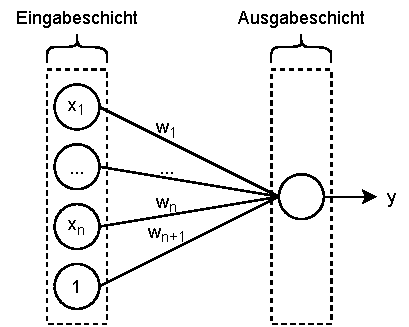
\includegraphics[width=0.5\textwidth]{content/images/FFNN.pdf}}
\caption{Einschichtiges Feedforward-Netz Eingabeschicht, Bias und einer Ausgabeschicht mit einem Neuron}
\label{f2.1}
\end{figure}

In Abbildung \ref{f2.1} ist das ein einfaches einschichtiges Feedforward-Netz mit einer Eingabeschicht und einer Ausgabeschicht mit einem Neuron dargestellt. Dieses Netz nimmt als Eingabe einen Featurevektor $\vec{x} = \left(\begin{array}{ccc} x_1 & \cdots & x_n \end{array} \right)^T$ und berechnet in diesem Fall als Ausgabe eine einzelne Zahl $y$. $y$ berechnet sich wie folgt:

\begin{equation}
y = \sigma \left( \left( \sum_{i=1}^{n} w_i \cdot x_i \right) + w_{n+1} \cdot 1 \right)
\label{eq2.1}
\end{equation} 

Als Erstes werden alle Werte der vorherigen Schicht, die mit dem Neuron in der aktuellen Schicht verbunden sind, mit den Gewichten an den jeweiligen Kanten gewichtet und aufsummiert. Dazu wird der sogenannte Bias addiert, welcher immer einen konstanten Wert besitzt (in dem Fall den Wert 1) und ebenfalls gewichtet mit dem Neuron in der Ausgabeschicht verbunden ist. Anschließend wird auf die gesamte Summe eine Aktivierungsfunktion $\sigma$ angewendet.

Bei mehr als nur einem Neuron in der Ausgabeschicht wird für jedes weitere Neuron analog vorgegangen und man erhält statt einer einzelnen Zahl einen Vektor als Ausgabe dieser Schicht. Handelt es sich um ein mehrschichtiges Feedforward-Netz, wird für jede Zwischenschicht bis zur Ausgabeschicht sukzessive diese beschriebene Technik angewendet, um den Ausgabevektor des Netzes zu erhalten.

Der Lernprozess eines solchen Feedforward-Netzes besteht darin mittels geeigneter Techniken die Gewichte anzupassen und dadurch den Fehler, den das Netz macht, zu minimieren, sodass die Ausgabe des Netzes die gewünschte Ausgabe approximiert.


\subsection{Convolutional Neural Networks}
\label{cnns}
Eine andere Art von Feedforward-Netzen sind die so genannten Convolutional Neural Networks, kurz CNNs. Diese Netze nutzen das mathematische Prinzip der Faltung (engl. Convolution), welches sich sowohl auf zweidimensionalen Daten wie Bildern, als auch auf eindimensionale Daten wie Zeitreihen anwenden lässt. Für diese Arbeit werden CNNs aber lediglich auf Bilddaten, also zweidimensionalen Daten betrachtet.

Convolutional Neural Networks werden, wie die zuvor beschriebenen Feedforward-Netze, erneut in Schichten angeordnet, jedoch werden bei den CNNs Convolutional Layer verwendet.

\begin{figure}[htbp]
\centerline{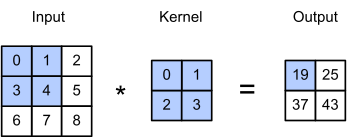
\includegraphics[width=0.5\textwidth]{content/images/convolution.png}}
\caption{Zweidimensionale Cross-Correlation auf einer Eingabe der Größe $3 \times 3$ mit einem Kernel der Größe $2 \times 2$. \cite{zhang_dive_2020}}
\label{f2.2}
\end{figure}

Ein Convolutional Layer ist eine Schicht, bei der ein Filter (Kernel) über die Eingabedaten (Input) geschoben wird. Dies wird auch Cross-Correlation oder Faltung (Convolution) genannt. Ein Beispiel für diese Cross-Correlation ist in Abbildung \ref{f2.2} dargestellt. Dabei wird der Kernel über den Eingabedaten platziert, die Werte des Kernels mit den darunterliegenden Werten der Eingabedaten multipliziert und alle Werte aufaddiert. Zusätzlich kann dann noch auf diese Summe eine Aktivierungsfunktion $\sigma$ angewendet werden. Anschließend wird der Kernel auf den Eingabedaten um eine festgelegte Schrittweite (strides) verschoben und die Prozedur wiederholt, bis der Kernel einmal über die gesamten Daten gelaufen ist. Das Ergebnis einer solchen Convolution wird auch Feature Map genannt.

Für einen Input $I$ und einen Kernel $K$ der Größe $M \times N$ kann das Ergebnis $S$ einer Cross-Correlation wie folgt formalisiert werden \cite{frochte_maschinelles_2019}:

\begin{equation}
S[i, j] = \sum_{m=1}^{M} \sum_{n=1}^{N} I[i+m, j+n] \cdot K[m, n]
\label{eq2.2}
\end{equation}

Die eckigen Klammern entsprechen in dieser Formel Zugriffe auf Elemente von Matrizen. Beispielsweise ist mit $S[i, j]$ der Wert der Feature Map in der $i$-ten Zeile und $j$-ten Spalte gemeint.

Besitzt der Input $I$ $C$ Channel (z.B. bei einem RGB-Bild $C = 3$), dann hat der Kernel $K$ die Größe $M \times N \times C$ und die Formel \ref{eq2.2} erweitert sich wie folgt:

\begin{equation}
S[i, j] = \sum_{c=1}^{C} \sum_{m=1}^{M} \sum_{n=1}^{N} I[i+m, j+n, c] \cdot K[m, n, c]
\label{eq2.3}
\end{equation}

Wird die Cross-Correlation, wie oben beschrieben, angewendet, ist die resultierende Feature Map kleiner als der Input, da der Kernel nicht über die Ränder hinauslaufen kann. Falls die Feature Map dieselbe Größe wie die Eingabe haben soll, kann ein Padding verwendet werden. Beim Padding werden die Eingabedaten an den Rändern mit Werten aufgefüllt. Eine Art des Paddings ist beispielsweise das Zero Padding, bei dem die Ränder der Eingabedaten mit Nullen aufgefüllt werden.



\section{Optimierte Schichten}
Neben den einfachen Schichten aus Neuronen oder den Convolutional Layern gibt es noch optimierte Schichten oder Kombinationen verschiedener Schichten, die eine Optimierung des Netzwerkes, in denen sie eingesetzt werden, erzielen sollen. 
Eine Auswahl solcher Optimierungen werden im folgenden vorgestellt und anschließend in Abschnitt \ref{architekturen} angewendet.


\subsection{Depthwise Separable Convolutions}
\label{depthwise_separable_convolutions}
In Abschnitt \ref{cnns} wurden die Convolutional Neural Networks mit den Convolutional Layern vorgestellt. Eine Depthwise Separable Convolution ist eine optimierte Variante der Standard-Convolution.

In der Formel \ref{eq2.3} ist dargestellt, wie eine Standard-Convolution auf Eingabedaten mit mehreren Channel arbeitet. Der Kernel der Größe $M \times N \times C$ führt auf jedem Channel eine Convolution durch und summiert im gleichen Schritt die Werte für jeden Channel zu einem Wert in der Feature Map. Bei der Depthwise Separable Convolution wurde diese Standard-Convolution aufgeteilt in die Depthwise Convolution und die Pointwise Convolution \cite{howard_mobilenets_2017}.

Die Depthwise Convolution führt auf Eingabedaten der Größe $H \times W \times C$ mit dem Kernel der Größe $M \times N \times C$ eine Convolution durch. Der Unterschied zur normalen Convolution besteht darin, dass die Ergebnisse der einzelnen Channel nicht aufsummiert werden. Dadurch bleiben die Channel in einer Depthwise Convolution erhalten. Diese Operation kann wie folgt formalisiert werden \cite{howard_mobilenets_2017}:

\begin{equation}
S[i, j, c] = \sum_{m=1}^{M} \sum_{n=1}^{N} I[i+m, j+n, c] \cdot K[m, n, c]
\label{eq2.4}
\end{equation}

Die Variable $c$ entspricht dabei dem Index eines Channel mit $1 \leq c \leq C$.

Nach dieser Depthwise Convolution Schicht folgt eine Pointwise Convolution Schicht, welche im Grunde eine normale Convolution mit einem Kernel der Größe $1 \times 1 \times C$ darstellt. Dieser Kernel bildet Linearkombinationen der einzelnen Channel und kombiniert somit die Channel zu einem einzelnen Channel. Die Menge an Channel der Feature Map einer Depthwise Separable Convolution Schicht wird durch die Anzahl der Kernel in der Pointwise Convolution Schicht gesteuert.

Durch das Aufspalten der Convolution in eine Depthwise Convolution und eine Pointwise Convolution erreicht die Depthwise Separable Convolution niedrigere Berechnungskosten und benötigt weniger Parameter \cite{howard_mobilenets_2017}. Der Faktor, um den die Berechnungskosten bei einer Depthwise Separable Convolution im Vergleich zu einer Standard-Convolution reduziert wird, beträgt \cite{howard_mobilenets_2017}:

\begin{equation}
\frac{1}{C_{out}} + \frac{1}{D_K^2}
\label{eq2.5}
\end{equation}

In Formel \ref{eq2.5} wird angenommen, dass der Kernel der Depthwise Convolution quadratisch mit der Höhe/Breite $D_K$ ist. $C_{out}$ entspricht der Anzahl an Channel in der Ausgabe der Depthwise Separable Convolution, welche sich durch die Anzahl an Kernel (Filter) der Pointwise Convolution Schicht ergibt.


\subsection{Linear Bottlenecks}
\label{linear_bottlenecks}
Eine Linear Bottleneck Schicht ist eine Kombination aus verschiedenen Convolutional Layern. Die Idee, welche hinter dieser Schicht steht, ist, dass angenommen wird, dass eine Menge von realen Bildern immer in eine niedrig-dimensionale Repräsentation eingebettet werden kann \cite{sandler_mobilenetv2_2019}. Also mit anderen Worten, die Menge an Bilder in eine komprimierte Darstellung überführt werden kann, bei denen die einzelnen Features einen höheren Informationsgehalt besitzen. Dies machen sich Linear Bottlenecks zunutze. 

Das grundlegende Prinzip hinter diesen Bottleneck Schichten ist, dass eine Eingabe durch eine Reihe von Convolutions in eine kleinere Darstellung (Bottleneck) gebracht wird, die anschließend alle wichtigen Informationen der Eingabe in komprimierter Form enthält.

\begin{figure}[htbp]
\centerline{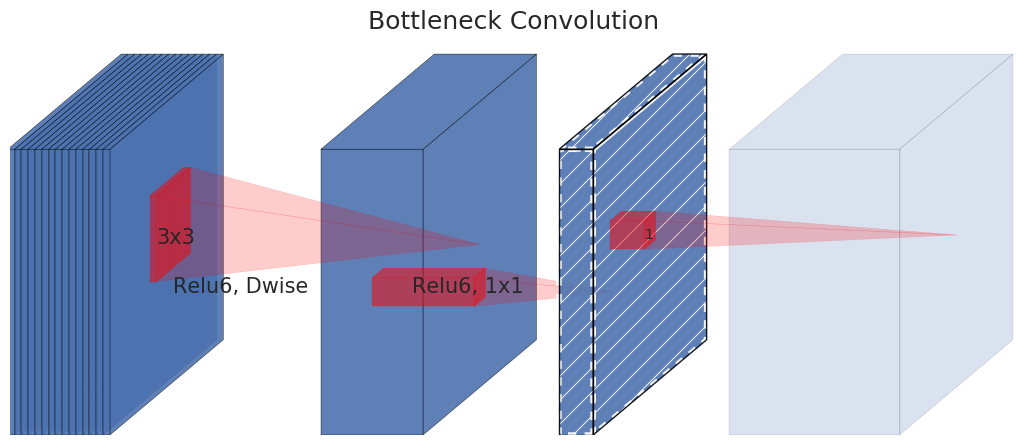
\includegraphics[width=0.6\textwidth]{content/images/bottleneck_block.png}}
\caption{Beispiel einer Linear Bottleneck Schicht. Die Breite jeder Schicht symbolisiert die Anzahl der Channel und auf den schraffierten Block wurde eine lineare Aktivierung angewendet. Der schwach sichtbare Block ist ein Block der nächsten Schicht. \cite{sandler_mobilenetv2_2019}}
\label{f2.3}
\end{figure}

Ein Beispiel für ein Linear Bottleneck aus dem Paper zu der Architektur MobileNetV2 \cite{sandler_mobilenetv2_2019} ist in Abbildung \ref{f2.2} dargestellt. Die Schicht besteht aus insgesamt 3 Convolutional Layern. Im ersten Schritt wird auf die Eingabe der Bottleneck Schicht eine nicht-lineare Aktivierungsfunktion (in dem Beispiel ReLU6) und anschließend eine Depthwise Convolution angewendet. Auf die Ausgabe der Depthwise Convolution wird erneut eine nicht-lineare Aktivierungsfunktion angewendet und es folgt eine Pointwise Convolution, welche die Eingabe auf eine komprimierte Repräsentation reduziert. Auf diese komprimierte Repräsentation wird zum Schluss eine lineare Aktivierungsfunktion angewendet und mittels Pointwise Convolution zu der Eingabe für die nächste Schicht transformiert.

\begin{figure}[htbp]
\centerline{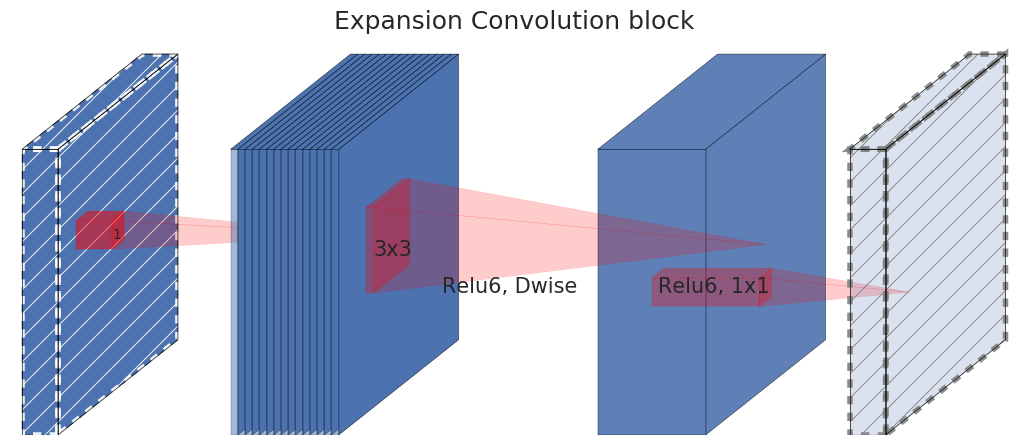
\includegraphics[width=0.6\textwidth]{content/images/expansion_block.png}}
\caption{Beispiel für einen Expansion Block. Die Breite jeder Schicht symbolisiert die Anzahl der Channel und auf die schraffierten Blöcke wurde eine lineare Aktivierung angewendet. Der schwach sichtbare Block ist ein Block der nächsten Schicht. \cite{sandler_mobilenetv2_2019}}
\label{f2.4}
\end{figure}

Werden mehrere von diesen Bottleneck Schichten hintereinandergeschaltet, ergibt sich eine Struktur, bei der immer wieder eine komprimierte Repräsentation in eine vergrößerte Repräsentation überführt wird und anschließend wieder in eine komprimierte Darstellung transformiert wird. Diese Blöcke werden auch Expansion Blöcke genannt und sind in Abbildung \ref{f2.4} dargestellt.

Das Paper zu MobileNetV2 beschreibt als Grund für die Anwendung der linearen Aktivierungsfunktion am Ende jeder Bottleneck Schicht, dass nicht-lineare Aktivierungsfunktionen zwar notwendig sind, um eine Nicht-Linearität des Modells zu erreichen, aber sie auch zu einer Zerstörung von Information führen. Außerdem haben Experimente gezeigt, dass die Anwendung einer linearen Aktivierungsfunktion in den Bottleneck Schichten zu einer Verbesserung des Netzwerkes führt \cite{sandler_mobilenetv2_2019}.


\subsection{Inverted Residuals}
\label{inverted_residuals}
Inverted Residuals \cite{sandler_mobilenetv2_2019} sind angelehnt an die Residual Blöcke der ResNet Architektur \cite{he_deep_2015}. Ein Residual Block in der ResNet Architektur nutzt ein Bottleneck Konstrukt, indem die Eingabe des Blocks mittels Convolutions komprimiert und anschließend wieder vergrößert wird. Zwischen der Eingabe und der Ausgabe des Residual Blocks befindet sich eine Abkürzung (Shortcut Connection), welche den Fluss der Gradienten im Trainingsprozess verbessert und es ermöglicht, tiefe Netze mit vielen Schichten besser zu trainieren \cite{he_deep_2015}.

Die Inverted Residual Blöcke verfolgen dieselbe Idee wie die Residual Blöcke beim ResNet, jedoch sind bei den Inverted Residual Blöcken die Schichten anders angeordnet. Ein Beispiel für ein Inverted Residual Block aus dem Paper zu der MobileNetV2 Architektur \cite{sandler_mobilenetv2_2019} ist in Abbildung \ref{f2.5} dargestellt. Der Unterschied bei den Inverted Residuals zu den Residual Blöcken ist, dass die Eingabe der Inverted Residual Schicht bereits die komprimierte Repräsentation ist, welche anschließend mittels einer Pointwise Convolution vergrößert wird. Darauf folgt eine Depthwise Convolution und erneut eine Pointwise Convolution, welche die Darstellung wieder komprimiert. Die Abkürzung befindet sich dabei zwischen dem Bottleneck am Eingang und der Bottleneck am Ausgang. Im Grunde handelt es sich um eine Expansion Schicht mit einer Abkürzung zwischen der Eingabe und der Ausgabe der Schicht.

\begin{figure}[htbp]
\centerline{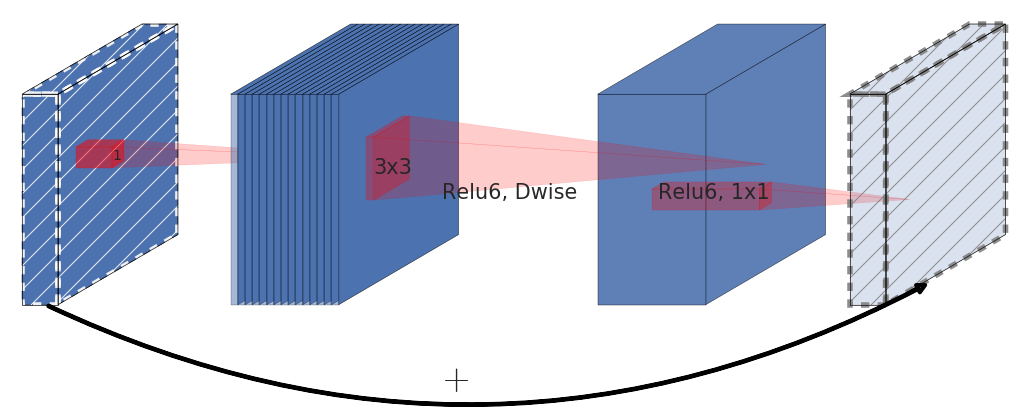
\includegraphics[width=0.6\textwidth]{content/images/inverted_residual.png}}
\caption{Inverted Residual Block. Die Breite jeder Schicht symbolisiert die Anzahl der Channel. \cite{sandler_mobilenetv2_2019}}
\label{f2.5}
\end{figure}

Bei der Abkürzung zwischen den Schichten handelt es sich lediglich um die Identitäts\-funktion. Das heißt, dass die Eingabe unverändert auf die Ausgabe addiert wird \cite{sandler_mobilenetv2_2019}.


\subsection{Squeeze-And-Excitation}
\label{squeeze_and_excitation}
Eine weitere Schicht sind die Squeeze-And-Excitation Schichten \cite{hu_squeeze-and-excitation_2019}. Der Grundgedanke hinter dieser Schicht ist es, die Beziehung zwischen den Kanälen (Channel) besser zu modellieren. Das Netzwerk soll die Möglichkeit haben wichtige Kanäle zu verstärken und weniger wichtige Kanäle abzuschwächen.

Diese Squeeze-And-Excitation Schicht, welche in Abbildung \ref{f2.6} dargestellt ist, kann nach beliebigen Transformationen $F_{tr}$ angewendet werden, die aus einer Eingabe $X$ der Größe $H' \times W' \times C'$ eine Feature Map $U$ der Größe $H \times W \times C$ generiert. Beispiele für mögliche Transformationen sind Convolutions oder Depthwise Convolutions.

\begin{figure}[htbp]
\centerline{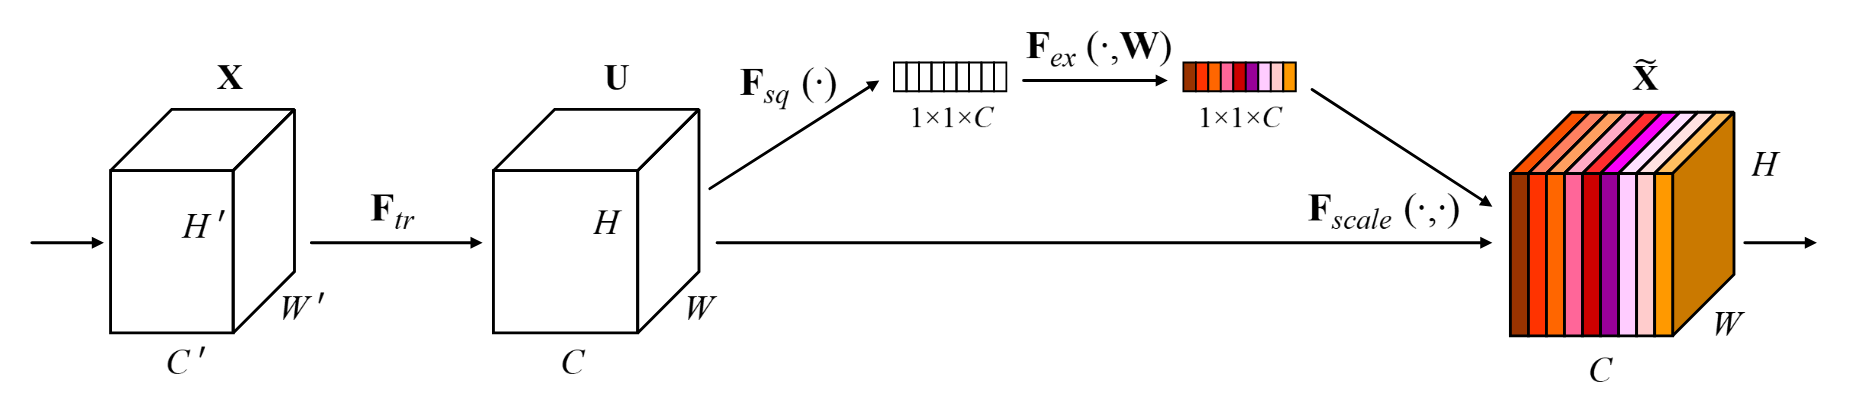
\includegraphics[width=0.9\textwidth]{content/images/squeeze_and_excitation.png}}
\caption{Ein Squeeze-And-Excitation Block. \cite{hu_squeeze-and-excitation_2019}}
\label{f2.6}
\end{figure}

Nach dieser Transformation wird auf die resultierende Feature Map die sogenannte Squeeze-Transformation angewendet, welche die Feature Map $U$ in eine Darstellung der Form $1 \times 1 \times C$ überführt. Dies kann zum Beispiel durch ein Global Average Pooling erreicht werden, welches für jeden Channel $u_c$ in $U = [u_1, u_2, \cdots, u_C]$ wie folgt berechnet wird \cite{hu_squeeze-and-excitation_2019}:

\begin{equation}
F_{sq}(u_c) = \frac{1}{H \cdot W} \sum_{i=1}^{H} \sum_{j=1}^{W} u_c[i, j]
\label{eq2.6}
\end{equation}

Darauf folgt die Excitation-Transformation, die auf das Ergebnis der Squeeze-Trans\-formation, analog zu den klassischen Feedforward-Netzen in Abschnitt \ref{FFNN}, mittels $F_{ex}$ eine Gewichtung $W$ und eine Aktivierung anwendet. Jedoch beinhaltet $F_{ex}$ noch ein Bottleneck, welcher in der Grafik \ref{f2.6} nicht ersichtlich ist. Das bedeutet $F_{ex}$ komprimiert zuerst mittels eines normalen Feedforward-Netzes die Darstellung der Größe $1 \times 1 \times C$ in einen Feature-Vektor der Größe $1 \times 1 \times \frac{C}{r}$ und wendet darauf eine Aktivierung an. Anschließend wird die komprimierte Darstellung wieder in die Darstellung der Größe $1 \times 1 \times C$ transformiert und erneut eine Aktivierung angewendet. $r$ ist dabei ein Parameter, der bestimmt, wie schmal der Bottleneck ist.

Die Ausgabe des Squeeze-And-Excitation Blockes wird nun mittels der Funktion $F_{scale}$ berechnet, welche lediglich die Channel aus der Feature Map $U$ mit den zugehörigen Channel aus dem Ergebnis von $F_{ex}$ multipliziert.



\section{Architekturen für Mobilgeräte}
\label{architekturen}
Nachdem die Grundlagen von künstlichen neuronalen Netzen und darauf aufbauende optimierte Schichten besprochen wurden, werden nun konkrete Architekturen für Convolutional Neural Networks vorgestellt, dessen Zielplattform mobile und eingebettete Systeme sind. Im Wesentlichen werden in diesem Abschnitt die verschiedenen MobileNet Varianten \cite{howard_mobilenets_2017, sandler_mobilenetv2_2019, howard_searching_2019} und die EfficientNet \cite{tan_efficientnet_2020} Architektur besprochen.


\subsection{MobileNet}
\label{mobilenet}
MobileNet \cite{howard_mobilenets_2017} ist eine Architektur aus dem Jahr 2017, welche von Entwicklern bei Google entwickelt wurde. Die Entwickler haben sich zum Ziel gesetzt, dem Trend, immer tiefere CNN Architekturen für eine gesteigerte Genauigkeit zu entwickeln, entgegenzuwirken, um die Verwendung von CNN Modellen auf mobilen und eingebetteten Systemen möglich zu machen. Dabei setzen sie den Hauptfokus bei der Entwicklung auf das Optimieren der Latenz, anstatt sich nur auf das Optimieren der Größe zu konzentrieren. Um dieses Ziel zu erreichen, haben die Entwickler die Architektur hauptsächlich aus Depthwise Separable Convolutions (siehe Abschnitt \ref{depthwise_separable_convolutions}) aufgebaut, welche die Berechnungskosten und die Größe des Netzwerkes stark reduzieren \cite{howard_mobilenets_2017}.

\begin{figure}[htbp]
\centerline{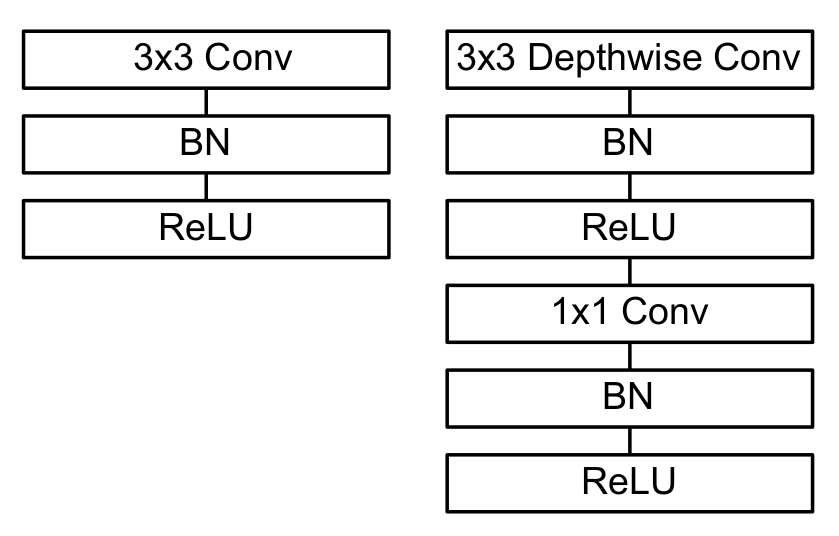
\includegraphics[width=0.3\textwidth]{content/images/mobilenet_blocks.png}}
\caption{Hauptbausteine des MobileNets. Links ist eine Standard-Convolution und rechts ist die Depthwise Separable Convolution. BN steht für Batch Normalisierung \cite{ioffe_batch_2015} und ReLU ist die ReLU Aktivierungsfunktion. \cite{howard_mobilenets_2017}}
\label{f2.7}
\end{figure}

Die MobileNet Architektur ist wie folgt aufgebaut. Sie beginnt mit der in Abbildung \ref{f2.7} dargestellten Standard-Convolution. Darauf folgen dann 13 Depthwise Separable Convolutions. Danach wird ein Average Pooling durchgeführt und das Ergebnis dieser Pooling-Operation wird mittels eines klassischen Feedforward-Netzes (Fully-Connected Layer) und einer Softmax Aktivierung als Klassifikator genutzt.

Um die Größe des MobileNets variieren zu können, gibt es noch einen Breitenmultiplikator (width multiplier) $\alpha$ und einen Auflösungsmultiplikator (resolution multiplier) $\rho$. Der Breitenmultiplikator skaliert gleichmäßig die Breite jeder Schicht, indem sich die Anzahl an Eingabe-Channel $M$ und Ausgabe-Channel $N$ in jeder Schicht zu $\alpha M$ und $\alpha N$ skalieren lassen.
Der Auflösungsmultiplikator $\rho$ wird in der Regel implizit gesetzt, indem die Auflösung des Eingabebildes verändert wird.


\subsection{MobileNetV2}
Im Jahr 2018 folgte auf die MobileNet Architektur die Nachfolgearchitektur MobileNetV2 \cite{sandler_mobilenetv2_2019}. Neben den Depthwise Separable Convolutions, welche bereits in der MobileNet Architektur Anwendung fanden, werden in dieser Architektur noch die Linear Bottlenecks (Abschnitt \ref{linear_bottlenecks}) und Inverted Residuals (Abschnitt \ref{inverted_residuals}) hinzugefügt.

Als Hauptbaustein nutzt die MobileNetV2 Architektur die Expansion Schicht mit residualer Verbindung wie sie in Abbildung \ref{f2.5} dargestellt ist. Diese Expansion Schichten werden in dem Paper auch Bottleneck Residual Block genannt. Mittels diesen Bottleneck Schichten wir nun die Architektur ähnlich zu MobileNet aufgebaut. 

Als erste Schicht kommt eine normale Standard-Convolution. Darauf folgen 17 Bottleneck Schichten. Von diesen Bottleneck Schichten besitzen alle Schichten, dessen Eingaben dieselbe Größe hat wie die Ausgaben, eine residuale Verbindung. Das ist für alle Bottleneck Schichten mit einer Schrittweite (Stride) von 1 der Fall. Bei den anderen Bottleneck Schichten handelt es sich um einfache Expansion Schichten. Nach diesen 17 Bottleneck Schichten folgt eine Pointwise Convolution und ein Average Pooling. Zur Klassifikation wird als letzte Schicht eine Pointwise Convolution verwendet. Als Aktivierungsfunktion wird in dieser Architektur ReLU6 eingesetzt.

Genau wie die MobileNet Architektur gibt es bei der MobileNetV2 Architektur den Breitenmultiplikator (width multiplier) $\alpha$ und den Auflösungsmultiplikator (resolution multiplier) $\rho$, die ermöglichen die Größe und Berechnungskosten der Architektur auf die Bedürfnisse anzupassen.


\subsection{MobileNetV3}
\label{mobilenetv3}
MobileNet und MobileNetV2 sind beides Architekturen, welche manuell von Menschen erdacht und konzipiert wurden. Die MobileNetV3 Architektur aus dem Jahr 2019 hingegen wurde mittels einer Platform-Aware Neural Architecture Search (Platform-Aware NAS) entwickelt \cite{howard_searching_2019}. Zusätzlich wurden noch einige manuelle Anpassungen vorgenommen. Von der MobileNetV3 Architektur gibt es eine kleine (Small) und eine große (Large) Variante.

Als Hauptbaustein der MobileNetV3 Architektur wird eine Linear Bottleneck Schicht mit Squeeze-And-Excitation und Inverted Residual verwendet wie in Abbildung \ref{f2.8} dargestellt. Als nichtlineare Aktivierungsfunktion wird dabei eine modifizierte Variante der Swish Aktivierungsfunktion \cite{howard_searching_2019} genutzt.

\begin{figure}[htbp]
\centerline{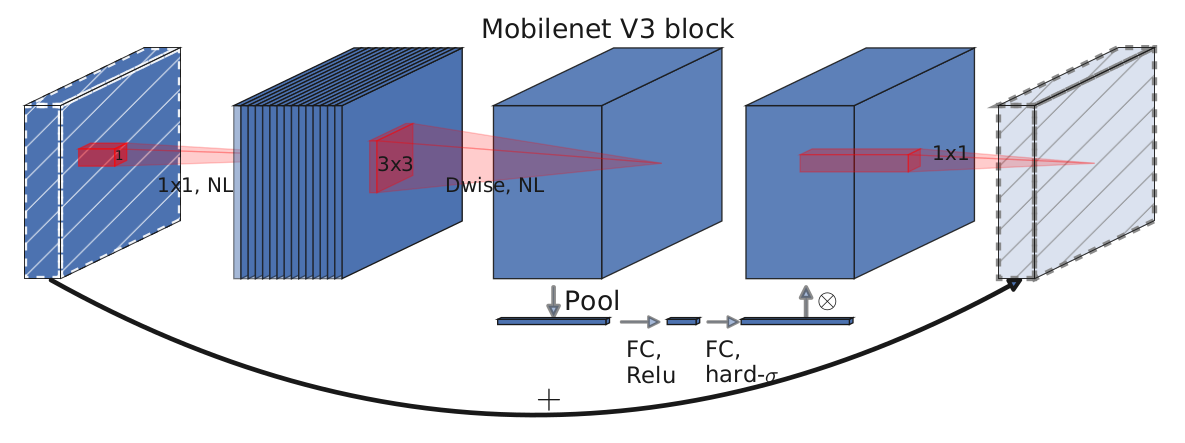
\includegraphics[width=0.7\textwidth]{content/images/mobilenetv3_block.png}}
\caption{Linear Bottleneck Schicht mit Squeeze-And-Excitation und Inverted Residual. \cite{howard_searching_2019}}
\label{f2.8}
\end{figure}

\subsubsection{MobileNetV3 Large}
Für die große Variante der MobileNetV3 Architektur wurde als Grundlage die durch Platform-Aware NAS gefundene Architektur MnasNet-A1 \cite{tan_mnasnet_2019} gewählt. Diese Architektur wurde mittels NetAdapt Algorithmus \cite{howard_searching_2019} weiter optimiert.
Anschließend wurden noch einige manuelle Anpassungen vorgenommen. 

Zu den manuellen Anpassungen gehören, dass teure Schichten überarbeitet wurden, indem die Anzahl der Filter der ersten Schicht verringert wurde und die letzten Schichten überarbeitet wurden, um eine geringere Latenz zu erreichen. Außerdem wurde ReLU6 als nichtlineare Aktivierungsfunktion durch eine modifizierte Variante der Swish Aktivierungsfunktion ersetzt, um die Genauigkeit der Architektur zu verbessern. Zusätzlich wurde die Skalierung des Squeeze-And-Excitation Bottlenecks angepasst.

Die MobileNetV3-Large Variante ist für mobile Plattformen mit einer größeren Anzahl an Ressourcen ausgelegt.


\subsubsection{MobileNetV3 Small}
Die kleine Variante des MobileNetV3 richtet sich an kleinere Plattformen mit einer geringen Menge an Ressourcen. Dazu baut diese Architektur nicht wie die große Variante auf der MnasNet-A1 Architektur auf, sondern wurde durch einen neuen Platform-Aware NAS Durchlauf gefunden. Platform-Aware Neural Architecture Search ist eine Technik, bei der eine optimale Architektur für eine bestimmte Plattform gesucht wird. Bei der MobileNetV3 Small Variante wurde bei dem NAS Algorithmus die Latenz und Genauigkeit der Architekturen auf real existierenden Mobilgeräten getestet und optimiert. Anschließend wurden dieselben Optimierungen wie auch bei der großen Variante angewendet.


\subsection{EfficientNet}
\label{efficientnet}
Eine weitere Architektur, welche mittels Neural Architecture Search entwickelt wurde, ist die EfficientNet Architektur aus dem Jahr 2019 \cite{tan_efficientnet_2020}. Die Entwickler haben sich bei dieser Architektur das Ziel gesetzt, eine Methode zu entwickeln, welche es erlaubt diese Architektur zu vergrößern und dabei eine bessere Genauigkeit zu erzielen, aber auch eine möglichst effiziente Architektur beizubehalten. Dazu haben sie die Compound Scaling Methode entwickelt.

Viele Architekturen lassen sich entweder nur in der Breite (Anzahl an Channel in den Schichten), in der Tiefe (Anzahl der Schichten) oder mittels der Auflösung des Eingabebildes skalieren. Beispielsweise lässt sich die MobileNet Architektur, wie in Abschnitt \ref{mobilenet} beschrieben, lediglich in der Breite und der Auflösung skalieren.
Die Idee hinter dem Compound Scaling ist es alle drei Arten der Skalierung zu verwenden, um eine Architektur gleichmäßig zu skalieren. Beim Compound Scaling wird ein Compound Koeffizient $\phi$ und Konstanten $\alpha$, $\beta$, $\gamma$ verwendet. Für die Konstanten muss gelten $\alpha \geq 1 \land \beta \geq 1 \land \gamma \geq 1$ und $\alpha \cdot \beta^2 \cdot \gamma^2 \approx 2$. Konkrete Werte für Konstanten $\alpha$, $\beta$, $\gamma$ wurden mittels einer Grid-Search ermittelt.
Anschließend wird die gegebene Basisarchitektur nach den folgenden Regeln skaliert \cite{tan_efficientnet_2020}:

\begin{itemize}
\item Tiefe: $d = \alpha^\phi$
\item Breite: $w = \beta^\phi$
\item Auflösung: $r = \gamma^\phi$
\end{itemize}

Um dieses Compound Scaling anwenden zu können, haben die Entwickler als Erstes mittels NAS Algorithmus eine Basisarchitektur entwickelt. Im Gegensatz zu MobileNetV3 wurde die Neural Architecture Search aber nicht für eine spezielle Hardware durchgeführt. Aus diesem Grund wurde anstelle nach Latenz und Genauigkeit nach Anzahl an Gleitkommazahlen-Operationen und Genauigkeit optimiert. Durch diese Suche ergab sich die Basisarchitektur EfficientNet-B0. Diese Architektur nutzt ähnlich wie die MobileNetV3 Architektur als Hauptbaustein die Linear Bottleneck Schichten mit Squeeze-And-Excitation und Inverted Residual. Als nichtlineare Aktivierungsfunktion wird die Swish Aktivierungsfunktion genutzt.

Auf Basis der EfficientNet-B0 Architektur wurden mittels der Compound Scaling Methode weitere Architekturen mit aufsteigender Anzahl an Parametern abgeleitet. Insgesamt gibt es 8 Architekturen (EfficientNet-B0 bis EfficientNet-B7), welche mit unterschiedlichen Werten für $\phi$ ermittelt wurden. Durch die Einschränkung $\alpha \cdot \beta^2 \cdot \gamma^2 \approx 2$ beim Compound Scaling gilt, dass wenn die Basisarchitektur mit einem $\phi$ vergrößert wird, vergrößert sich die Anzahl an Gleitkommazahlen-Operationen ungefähr um $2^\phi$. So können die Berechnungskosten auf die vorhandenen Ressourcen eingestellt werden.

Auf den normalen EfficientNet Architekturen aufbauend wurden im Jahr 2020 zusätzlich die EfficientNet-lite \cite{liu_higher_2020} Architekturen veröffentlicht. Die Idee hinter den EfficientNet-lite Architekturen ist auf dem EfficientNet basierende Architekturen bereitzustellen, die eine höhere Kompatibilität mit verschiedener Hardware aufweisen, weniger Parameter besitzen und sich besser quantisieren lassen. Dazu wurden zum einen die Squeeze-And-Excitation Module entfernt, da sie teilweise nicht gut unterstützt werden und zum anderen wurde die Swish Aktivierungsfunktion durch ReLU6 ausgetauscht, um eine bessere Quantisierbarkeit zu ermöglichen. Außerdem wurden einige Parameter beim Compound Scaling ausgeschlossen, da dadurch die Anzahl an Berechnungen verringert wird. Es gibt insgesamt fünf EfficientNet-lite Varianten (EfficientNet-lite0 bis EfficientNet-lite4), welche aufsteigend viele Parameter besitzen.



\section{Quantisierung}
\label{quantisierung}
Im vorherigen Abschnitt wurden Architekturen vorgestellt, welche versprechen eine gute Performance auf mobiler und eingebetteter Hardware zu besitzen. Zusätzlich zum Aufbau der Architektur lässt sich mittels Techniken wie Quantisierung die Effizienz in Bezug auf Inferenzgeschwindigkeit und Speicherbedarf weiter optimieren.

Bei der Quantisierung geht es darum, die Gewichte und Aktivierungen eines Netzwerkes in eine Darstellung zu überführen, welche weniger Bits als die ursprüngliche Darstellung benötigen. Ein Beispiel für eine Quantisierung ist, das Überführen eines Netzwerkes, welches 32 Bit Fließkommazahlen für die Gewichte/Aktivierungen verwendet, in ein Netzwerk, welches lediglich 8 Bit Integer verwendet. Dabei können die Gewichte und Aktivierungen in unterschiedliche Bitlängen quantisiert werden \cite{jacob_quantization_2017}.

Quantisierung hat dadurch den Vorteil, dass durch die verkleinerte Repräsentation der Gewichte und Aktivierungen der Gesamtspeicherbedarf eines Netzwerkes sinkt. Außerdem wird durch die Quantisierung in Integer die Geschwindigkeit des Netzwerkes auf Hardware, welche lediglich Integer-Operationen unterstützt, erhöht \cite{jacob_quantization_2017}.

Um ein gegebenes Netzwerk zu quantisieren, wurden im Laufe der Zeit verschiedene Ansätze entwickelt \cite{guo_survey_2018}. In dieser Arbeit wird im Wesentlichen das Quantisierungsschema der TensorFlow Bibliothek vorgestellt \cite{jacob_quantization_2017}. Dieses Quantisierungsschema bietet zwei Möglichkeiten eine Quantisierung vorzunehmen. Zum einen kann ein bereits vollständig trainiertes und bisher noch nicht quantisiertes Netz nachträglich quantisiert werden. Dies wird als Post-Training Quantization bezeichnet. Eine andere Möglichkeit, die als Quantization-Aware Training bezeichnet wird, ist das Trainieren eines Full-Precision Modells so als wäre es quantisiert. Im Folgenden werden diese beiden Möglichkeiten genauer betrachtet.


\subsection{Post-Training Quantization}
\label{post-training-quantization}
Bei der Post-Training Quantization wird als Grundlage ein bereits trainiertes neuronales Netz verwendet. Von diesem Netz werden dann die Gewichte und/oder Aktivierungen nachträglich quantisiert. Um dies zu erreichen wird ein reeller Wert $r$ (z.B. ein Gewicht des Netzes als 32 Bit Fließkommazahl) wie folgt durch einen quantisierten Wert $q$ (z.B. 8 Bit Integer) dargestellt \cite{jacob_quantization_2017}:

\begin{equation}
r = S (q - Z)
\label{eq2.7}
\end{equation}

In dieser Formel sind $S$ und $Z$ Konstanten. Dabei steht $S$ für "`scale"' und entspricht demselben Typ wie der nicht quantisierte Wert $r$. Die Konstante $Z$ steht für "`zero-point"' und hat denselben Typ wie der quantisierte Wert $q$. $Z$ entspricht dem quantisierten Wert für den die reelle Zahl 0 ($r = 0$). Diese beiden Konstanten werden auch als Quantisierungsparameter bezeichnet und für jede Gewichtsmatrix neu bestimmt.

Mit dieser Formel ist es möglich, sämtliche Parameter des Modells zu quantisieren, indem man jeden zu quantisierenden Parameter $r$ als einen Wert $q$ mit den Konstanten $S$ und $Z$ darstellt. Aufbauend auf diesem Quantisierungsschema lassen sich effiziente Operationen wie Matrizenmultiplikationen definieren, welche nur auf den quantisierten Werten (Integer) arbeiten \cite{jacob_quantization_2017}.

Wird mittels dieses Schemas ein bereits trainiertes Full-Precision Modell nachträglich quantisiert, funktioniert dies bei großen Modellen häufig gut. Bei kleineren Modellen kann dies zu größeren Einbußen in der Genauigkeit des Modells führen \cite{jacob_quantization_2017}. Gründe dafür können zum einen sein, dass die Gewichte zwischen den einzelnen Ausgabekanälen einer Schicht zu weit voneinander entfernt sind. Zum anderen kann es aber auch daran liegen, dass es Ausreißer in den Gewichten gibt, welche die Präzision der anderen Gewichte in quantisierter Form verschlechtern \cite{jacob_quantization_2017}.


\subsection{Quantization-Aware Training}
\label{quantization_aware_training}
Um diesem Problem entgegen zu wirken gibt es den Ansatz des Quantization-Aware Training. Bei diesem Ansatz wird ein Full-Precision Modell trainiert und dabei die Auswirkungen von Quantisierung lediglich simuliert.

Dazu wird beim Training im Foreward-Pass die Eingabe, Gewichte und Aktivierungsfunktionen so berechnet als wäre das Model quantisiert. Anschließend wird der Fehler berechnet, den das Netzwerk gemacht hat und beim Backward-Pass wie bei einem nicht quantisierten Full-Precision Modell die Gewichte angepasst. Die Gewichte werden jedoch in dem Typ des nicht quantisierten Modells gespeichert und können somit beim Backward-Pass sehr feingranular angepasst werden.

Nach diesem Training ergibt sich ein trainiertes Full-Precision Modell, welches so trainiert wurde als wäre es quantisiert. Dieses Modell kann anschließend mittels Post-Training Quantization in eine quantisierte Repräsentation überführt werden.



\section{Pruning}
\label{pruning}
Neben der Quantisierung gibt es als weitere Optimierungstechnik das sogenannte Pruning (Beschneiden). Beim Pruning wird ein Netzwerk optimiert, indem Verbindungen unterbrochen werden, welche keinen signifikanten Beitrag zur Ausgabe des Netzwerkes leisten. Mit Verbindungen unterbrechen ist in dem Zusammenhang das auf 0 setzen von Gewichten gemeint. Durch ein angemessenes Pruning kann die Größe eines Modells drastisch reduziert werden mit meist geringen Einbußen in der Genauigkeit \cite{zhu_prune_2017}.

Um ein gegebenes Netzwerk zu prunen gibt es verschiedene Ansätze \cite{gale_state_2019, mishra_survey_2020}. In dieser Arbeit wird der Ansatz des Magnitude Pruning \cite{zhu_prune_2017} genauer betrachtet, da es sich beim Magnitude Pruning um einen einfachen und effektiven Ansatz handelt, welcher trotz der Einfachheit gute Ergebnisse erzielt.

\subsection{Magnitude Pruning}
\label{magnitude_pruning}
Beim Magnitude Pruning wird bei einem gegebenen Netzwerk für jede Gewichtsmatrix eine binäre Maske derselben Größe erzeugt. Die einzelnen Einträge in dieser binären Maske geben an, welche der Gewichte beim Training berücksichtigt werden und welche nicht. Anschließend werden die einzelnen Gewichte nach ihrem Wert sortiert und in der Maske die kleinsten Gewichte auf 0 gesetzt bis ein Prozentsatz $s$ (Sparsity) erreicht wurde, welcher den Anteil der auf 0 gesetzten Gewichte in dem Netzwerk angibt \cite{zhu_prune_2017}.

In der Magnitude Pruning Methode aus dem Jahr 2017 \cite{zhu_prune_2017}, welche hier beschrieben wird, besteht der Pruningprozess aus einer mehrfachen wechselweisen Abfolge von Pruning und Training. Dazu wurde ein Algorithmus zum schrittweisen Prunen von neuronalen Netzen entwickelt. Dieser Algorithmus beginnt bei einer Sparsity von $s_i$ Prozent und erhöht $n$ Mal alle $\Delta t$ Schritte den Anteil der auf 0 gesetzten Gewichte bis zu einem gewünschten Prozentsatz $s_f$. Der Startpunkt, ab wann der Pruningprozess im Verlauf des Trainingsprozesses beginnt, kann mit dem Parameter $t_0$ festgelegt werden. Der Anteil $s_t$ der auf 0 gesetzten Gewichte im Pruningschritt $t$ wird nach folgender Formel berechnet \cite{zhu_prune_2017}:

\begin{eqnarray}
s_t = s_f + \left( s_i - s_f \right) \left( 1 - \frac{t - t_0}{n \Delta t} \right)^3
& \textrm{für} 
& t \in \{ t_0, t_0 + \Delta t, \cdots, t_0 + n \Delta t \}
\label{eq2.8}
\end{eqnarray}

Die Idee hinter diesem schrittweisen Pruning ist, dass nach jedem Pruningschritt das Netzwerk durch das anschließende Training die Möglichkeit bekommt sich an diesen Eingriff anzupassen und mögliche Verluste durch das Pruning auszugleichen bevor erneut ein Pruningschritt folgt. In Abbildung \ref{f2.9} ist ein Beispiel für einen schrittweisen Pruningvorgang nach der Formel \ref{eq2.8} dargestellt, in der zu erkennen ist, dass am Anfang des Pruningprozesses die Anzahl der Gewichte, die auf 0 gesetzt werden, größer ist und im Verlauf des Prozesses das Netz immer weniger stark gepruned wird, bis die gewünschte Sparsity $s$ erreicht wurde. Der Grund dafür ist, dass angenommen wird, dass am Anfang des Pruningvorgangs viele unwichtige Gewichte im Netzwerk existieren und mit zunehmender prozentualer Sparsity weniger unwichtige Gewichte im Netz vorhanden sind \cite{zhu_prune_2017}.

\begin{figure}[htbp]
\centerline{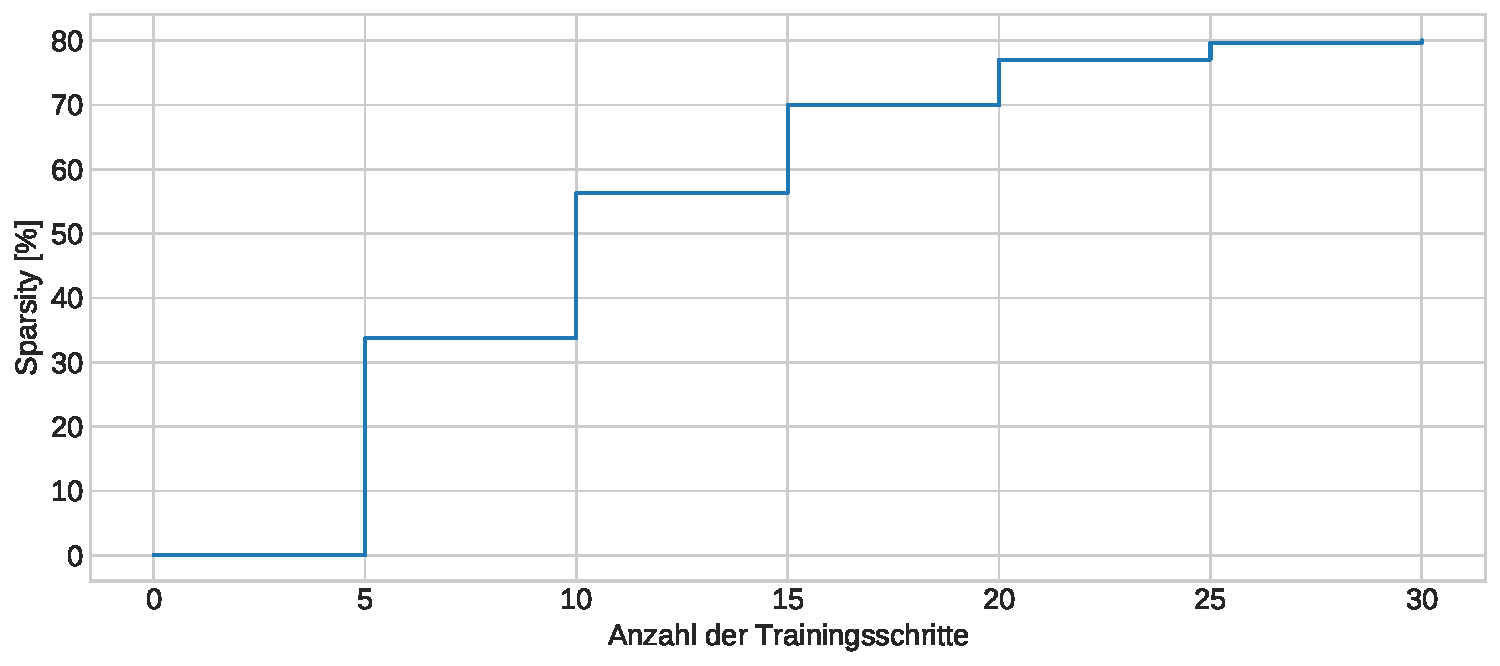
\includegraphics[width=0.9\textwidth]{content/images/magnitude_pruning_schedule.pdf}}
\caption{Ein Beispiel für einen Pruningprozess nach der Formel \ref{eq2.8} mit den Parametern $s_i = 0$, $s_f = 80$, $t_0 = 0$, $\Delta t = 5$ und $n = 6$.}
\label{f2.9}
\end{figure}

\chapter{Ansatz \& Implementierung}
\label{ansatz_und_implementierung}
Im Folgenden wird erläutert, wie vorgegangen wird, um die Fragestellung nach den Auswirkungen von Quantisierung und Pruning auf mobile Architekturen zu beantworten und wie die einzelnen Optimierungstechniken auf die ausgewählten Architekturen angewendet werden. Dazu wird im ersten Abschnitt beschrieben was das grundsätzliche Vorgehen in dieser Arbeit ist, um die verschiedenen Architekturen miteinander vergleichen zu können. Anschließend wird kurz die für die Implementierung verwendete Bibliothek TensorFlow erläutert. Im dritten Abschnitt werden die Trainingskonfiguration und der Datensatz beschrieben, mit denen alle Architekturen trainiert werden. Zum Schluss wird in den letzten beiden Abschnitten darauf eingegangen, wie genau die Quantisierung und das Pruning der vorgestellten Architekturen implementiert und durchgeführt werden.



\section{Vorgehen}
\label{vorgehen}
In dieser Arbeit wird grundsätzlich wie folgt vorgegangen: Als Erstes werden die im Abschnitt \ref{architekturen} vorgestellten Architekturen auf einem ausgewählten Datensatz trainiert und die trainierten Modelle gesichert.
Auf Basis dieser vortrainierten und gesicherten Modelle werden anschließend die Optimierungstechniken Quantisierung und Pruning angewendet. Dazu werden die Modelle immer ausgehend von den vortrainierten Modellen quantisiert, gepruned und sowohl zuerst gepruned als auch anschließend quantisiert. So ergeben sich die folgenden Kombinationen von Modelloptimierungen:

\begin{itemize}
\item vortrainiert
\item vortrainiert und quantisiert
\item vortrainiert und gepruned
\item vortrainiert, gepruned und quantisiert
\end{itemize}

Die 4 Kombinationen werden anschließend untereinander verglichen und es wird untersucht, was die Auswirkungen der architekturellen Besonderheiten der mobilen Architekturen unter Anwendung von Quantisierung und Pruning sind.



\section{TensorFlow}
Für die Implementierung wird die Python Bibliothek TensorFlow \footnote{\url{https://www.tensorflow.org/}} verwendet. TensorFlow stellt eine Reihe von Implementierungen verschiedener Netzwerke und Algorithmen des maschinellen Lernens bereit. Dazu gehören auch Implementierungen der in Abschnitt \ref{architekturen} vorgestellten Architekturen, was eine händische Implementierung dieser Architekturen überflüssig macht.


\subsection{TensorFlow Lite}
Um die Quantisierung von Modellen zu ermöglichen, bietet TensorFlow (\lstinline{tf}) ein Modul namens TensorFlow Lite (\lstinline{tf.lite}). Dieses Modul ist auf die Entwicklung von Modellen für mobile und eingebettete Systeme wie Mobiltelefone oder Mikrocontroller spezialisiert.
Implementiert ist in diesem Modul beispielsweise die Post-Training Quantisierung. Außerdem stellt TensorFlow Lite den TFLite FlatBuffer als effiziente Datenstruktur zum Speichern von Modellen zur Verfügung. Die TFLite FlatBuffer Datenstruktur ist eine optimierte Variante der FlatBuffer Bibliothek \footnote{\url{https://google.github.io/flatbuffers/flatbuffers\_white\_paper.html}}. Bei dem FlatBuffer Format handelt es sich um ein binäres Format, welches im Gegensatz zu z.B. JSON oder XML nicht menschenlesbar ist, aber dadurch mit wenig Overhead auskommt und aus diesem Grund besonders speicherplatzeffizient ist.
 

\subsection{TensorFlow Model Optimization Toolkit}
Für das Pruning wird zusätzlich noch das TensorFlow Model Optimization Toolkit \footnote{\url{https://www.tensorflow.org/model\_optimization}} benötigt. Diese Bibliothek stellt einige Algorithmen bereit, um Modelle des maschinellen Lernens zu optimieren. Dazu zählt beispielsweise das Quantization-Aware Training, welches in Abschnitt \ref{quantization_aware_training} beschrieben wurde und das Magnitude Pruning aus Abschnitt \ref{magnitude_pruning}.



\section{Training}
\label{training}
In dem weiteren Verlauf der Arbeit werden ausschließlich die Standardvarianten der vorgestellten Architekturen betrachtet. Das bedeutet, dass keine Variationen des Breitenmultiplikators beim MobileNet und beim MobileNetV2 betrachtet werden, da dies lediglich die Anzahl an Parametern variiert, aber nichts grundsätzlich an der Architektur ändert. Aus demselben Grund wird beim EfficientNet ebenfalls nur das EfficientNet-B0 betrachtet, da die Varianten EfficientNet-B1 bis EfficientNet-B7 lediglich mittels Compound Scaling skaliert wurden, aber keine neuen Architekturen darstellen. Damit werden im Folgenden die Architekturen MobileNet, MobileNetV2, MobileNetV3 Large, MobileNetV3 Small und EfficientNet-B0 verwendet.

Diese Architekturen werden bereits von der TensorFlow Bibliothek (\lstinline{tf}) in dem Modul \lstinline{tf.keras.applications} implementiert und können einfach instanziiert werden. Beim Erzeugen einer Instanz dieser Architekturen kann über den \lstinline{weights}-Parameter angegeben werden, ob die Architektur mit vortrainierten Gewichten geladen werden soll oder ob lediglich eine zufällige Initialisierung der Gewichte erfolgen soll. Die vortrainieren Gewichte sind auf dem ImageNet Datensatz \cite{russakovsky_imagenet_2015} vortrainiert. Jedoch unterstützen die auf ImageNet vortrainierten MobileNet Architekturen keine Eingaben der Größe $32 \times 32 \times 3$ wie es bei dem verwendeten CIFAR-10 Datensatz (siehe Abschnitt \ref{datensatz}) der Fall ist. Aus diesem Grund werden in dieser Arbeit die Architekturen mit zufällig initialisierten Gewichten neu trainiert.

Um ein möglichst einheitliches Trainings-Setup für alle Architekturen zu schaffen, werden alle Architekturen mit denselben Trainingsparametern trainiert. Für die Trainingsdurchläufe wird der von allen vorgestellten Architekturen vorgeschlagene RMSprop Optimizer (\lstinline{tf.keras.optimizers.RMSprop}) \cite{howard_mobilenets_2017, sandler_mobilenetv2_2019, howard_searching_2019, tan_efficientnet_2020} mit einem Momentum von 0.9 verwendet. Da es sich bei der Aufgabe, welche die Netzwerke lernen sollen, um ein Klassifizierungsproblem mit mehr als zwei Klassen handelt, wird die Categorical Cross-Entropy Verlustfunktion (\lstinline{tf.keras.losses.CategoricalCrossentropy}) gewählt. Als Batch Size wird 64 verwendet. Die Learning Rate wird während des Trainings in 150 Epochen, beginnend bei einer initialen Learning Rate von $1 \cdot 10^{-3}$, linear auf 0 abgesenkt (\lstinline{tf.keras.optimizers.schedules.PolynomialDecay}). Diese Wahl der Parameter hat in der Arbeit am besten funktioniert, um alle Architekturen mit denselben Parametern trainieren zu können. Um ein Overfitting der Modelle während des Trainings abzumildern, wird das Training mittels EarlyStopping abgebrochen, wenn beim Training innerhalb von 50 Epochen keine Verbesserung des Verlustes auf den Testdaten erreicht wird (\lstinline{tf.keras.callbacks.EarlyStopping}).

Am Ende jedes Trainings wird das trainierte Modell abgespeichert, um in späteren Schritten ein Pruning oder eine Quantisierung darauf anzuwenden.


\subsection{Datensatz}
\label{datensatz}
Als Datensatz wird in dieser Arbeit der CIFAR-10 Datensatz \cite{krizhevsky_learning_2009} verwendet. Dieser Datensatz enthält insgesamt 60000 Farbbilder der Größe $32 \times 32$ Pixel. Die Bilder in dem Datensatz können in 10 Klassen eingeordnet werden: Flugzeug, Automobil, Vogel, Katze, Hirsch, Hund, Frosch, Pferd, Schiff und Lastkraftwagen. Zu jeder dieser Kategorien sind jeweils 6000 Bilder in dem Datensatz vorhanden. Der gesamte Datensatz ist zusätzlich noch aufgeteilt in eine Trainingsmenge und eine Testmenge. Die Trainingsmenge enthält insgesamt 50000 Bilder mit jeweils 5000 Bildern pro Klasse und die Testmenge enthält die restlichen 10000 Bilder. In Abbildung \ref{f3.1} ist je ein Beispielbild für jede Klasse dargestellt.

\begin{figure}[htbp]
\centerline{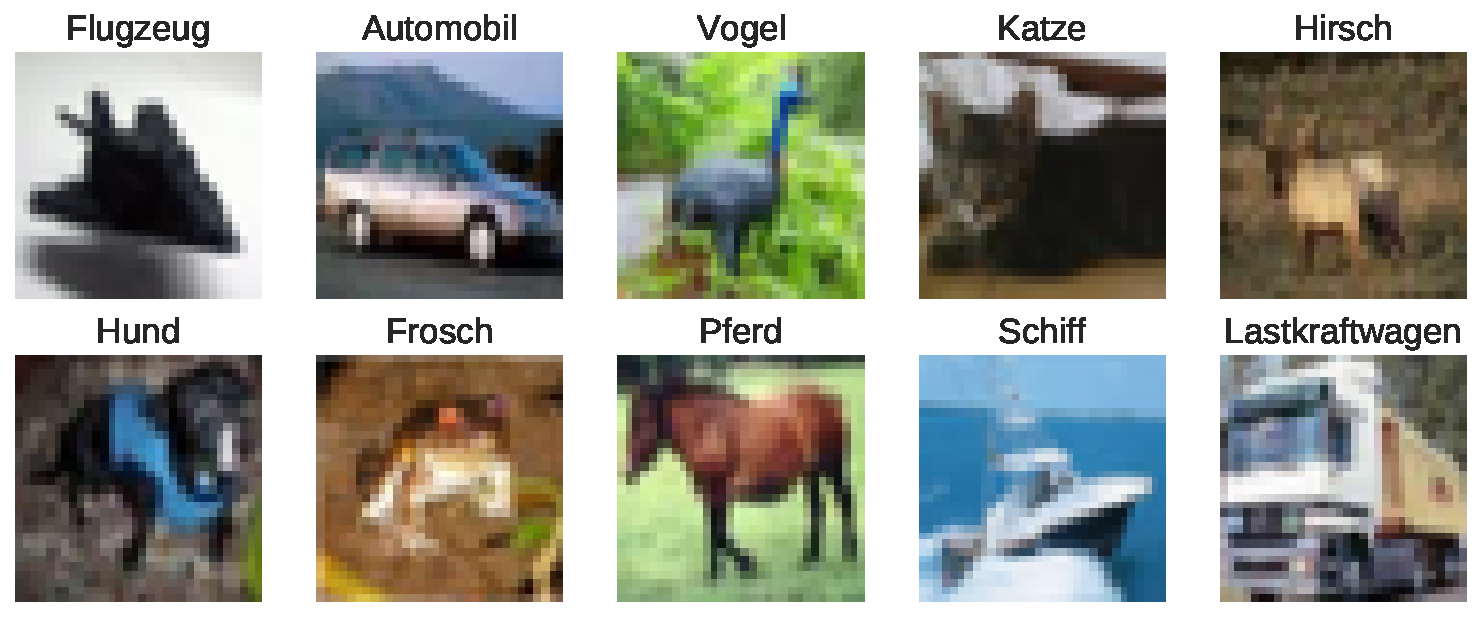
\includegraphics[width=0.8\textwidth]{content/images/cifar-10.pdf}}
\caption{Ein Beispielbild pro Klasse aus dem CIFAR-10 Datensatz.}
\label{f3.1}
\end{figure}

Der Grund, warum für diese Arbeit der CIFAR-10 Datensatz gewählt wurde, ist, dass für die Vergleiche der verschiedenen Architekturen untereinander und das Pruning viele Trainingsdurchläufe benötigt werden. Durch die geringe Anzahl und niedrige Auflösung der Bilder des CIFAR-10 Datensatzes ist ein einfaches Training möglich. Der häufig in der Literatur verwendete ImageNet Datensatz \cite{russakovsky_imagenet_2015} hingegen enthält insgesamt 1431167 hochauflösende Bilder und ist somit für diese Arbeit ungeeignet, da dieser durch die enorme Datenmenge die für diese Arbeit verfügbaren Kapazitäten überschreitet.



\section{Quantisierung}
\label{impl_quantisierung}
Zu der Quantisierung wurde in Abschnitt \ref{quantisierung} sowohl die Post-Training Quantisierung als auch das Quantization-Aware Training erläutert. Beim Quantization-Aware Training werden Modelle mittels simulierter Quantisierung von Grund auf trainiert. Hingegen kann die Post-Training Quantisierung direkt auf bereits trainierte Modelle angewendet werden, ohne ein erneutes Training zu erfordern. Aus zeitlichen Gründen wird in dieser Arbeit vorrangig die Post-Training Quantisierung betrachtet.

Ausgehend von einem 32 Bit Fließkomma Modell bietet TensorFlow für die Post-Training Quantisierung im Wesentlichen 3 Methoden an. Das ist zum einen die Post-Training Dynamic Range Quantization, bei der die Parameter des Modells lediglich für die Speicherung quantisiert werden und zur Inferenzzeit wieder in 32 Bit Fließkommazahlen konvertiert werden. Eine weitere Option die TensorFlow bietet ist das Quantisieren der Parameter in 16 Bit Fließkommazahlen. Als dritte Option bietet TensorFlow die Post-Training Integer Quantization an. Dazu gehört zum einen die Integer-Only Quantisierung, welche sämtliche Parameter und Aktivierungen in 8-Bit Integer quantisiert. Diese Integer-Only Quantisierung ist besonders wichtig für Hardware, welche nur Integer-Operationen unterstützt. Ein Beispiel für eine solche Integer-Only Hardware ist Googles Edge TPU \footnote{\url{https://cloud.google.com/edge-tpu}}. Zum anderen gehört zur Post-Training Integer Quantisierung auch die Float Fallback Quantisierung, welche ebenfalls wie die Integer-Only Quantisierung sämtliche Parameter und Aktivierungen in 8 Bit Integer quantisiert und lediglich die Ein- und Ausgabeschicht der Modelle im 32 Bit Fließkommaformat beibehält. In dieser Arbeit wird vorrangig die Post-Training Float Fallback Quantisierung betrachtet, da die EfficientNet Architekturen in TensorFlow derzeit noch nicht kompatibel mit der Integer-Only Quantisierung sind und durch die Quantisierung in 8 Bit Integer eine höhere Kompression der Modelle möglich ist als bei der Quantisierung in 16 Bit Fließkommazahlen.

Um diese Quantisierung durchzuführen stellt das TensorFlow Lite Modul den TFLiteConverter zur Verfügung (\lstinline{tf.lite.TFLiteConverter}). Eine Instanz dieses Konverters kann beispielsweise mit der Funktion \lstinline{tf.lite.TFLiteConverter.from_keras_model} erzeugt werden, welche als Parameter eine Instanz eines Keras Modells erwartet. Um dem erzeugten Konverter-Objekt mitzuteilen, dass das Modell quantisiert werden soll, muss das \lstinline{optimizations} Attribut des Objekts auf die Liste \lstinline{[ tf.lite.Optimize.DEFAULT ]} gesetzt werden. Für eine Float Fallback Quantisierung muss diesem erzeugten Konverter-Objekt zusätzlich ein repräsentativer Datensatz bekannt gemacht werden. Dieser repräsentative Datensatz sollte groß genug sein, um typische Werte für die Eingabedaten zu enthalten. Dabei kann es sich aber einfach um eine Untermenge der Trainingsdaten handeln. Der Datensatz wird anschließend von dem Konverter für Optimierungen bei der Quantisierung genutzt, wie beispielsweise das Vorhersehen von Wertebereichen der Eingabedaten. Anschließend kann auf dem Konverter-Objekt die \lstinline{convert()} Funktion aufgerufen werden, was letztendlich die Quantisierung und Konvertierung in das TFLite Format durchführt. Das resultierende TFLite Objekt kann anschließend als \lstinline{.tflite}-Datei gespeichert werden.

Neben der Quantisierung ist es mit dem \lstinline{TFLiteConverter} ebenfalls möglich trainierte Modelle ohne Anwendung von Quantisierung in das TFLite FlatBuffer Format zu konvertieren. Dazu muss erneut eine Instanz der Klasse \lstinline{tf.lite.TFLiteConverter} erstellt werden. Darauf muss anschließend direkt die \lstinline{convert()} Funktion aufgerufen werden, ohne irgendwelche Optimierungen zu spezifizieren.

Um eine Inferenz auf einem gespeicherten TFLite Modell durchzuführen, muss der TensorFlow Lite Interpreter (\lstinline{tf.lite.Interpreter}) verwendet werden. Dieser wird mit dem Pfad zu dem gespeicherten TFLite Modell instanziiert. Anschließend können mittels dieses Objektes Inferenzen auf dem geladenen Modell durchgeführt werden.



\section{Pruning}
\label{impl_pruning}
Das Pruning wird auf Grundlage der in Abschnitt \ref{training} trainierten Modelle durchgeführt. Dazu werden die Modelle geladen und erneut trainiert, wobei bei dem Training in regelmäßigen Abständen Gewichte auf 0 gesetzt werden. Dieses Pruning erfolgt nach dem Konzept des Magnitude Pruning, welches in Abschnitt \ref{magnitude_pruning} beschrieben wurde. Dazu wird das TensorFlow Model Optimization Toolkit (\lstinline{tfmot}) verwendet, welches in dem Modul \lstinline{tfmot.sparsity.keras} sämtliche Funktionalitäten enthält, um ein Magnitude Pruning durchzuführen.

Für das Magnitude Pruning nach dem TensorFlow Model Optimization Toolkit muss als Erstes jedes zu prunende Layer mit der Funktion \lstinline{prune_low_magnitude} aus dem Modul \lstinline{tfmot.sparsity.keras} markiert werden. Diese Funktion erwartet eine Schicht, die gepruned werden soll und zusätzlich ein \lstinline{PruningSchedule} Objekt, welches beschreibt, wie der Pruningprozess ablaufen soll. Diese Arbeit verwendet hier das in Abschnitt \ref{magnitude_pruning} beschriebene schrittweise Pruning, das mittels \lstinline{tfmot.sparsity.keras.PolynomialDecay} als \lstinline{PruningSchedule} Objekt implementiert wurde. Um nun jede Schicht mit der Funktion \lstinline{prune_low_magnitude} zu markieren, wird die \lstinline{tf.keras.models.clone_model} Funktion verwendet, welche ein Modell und eine Funktion als Parameter entgegennimmt und als Ergebnis ein neues Modell zurück gibt, welches durch die Funktionsanwendung der gegebenen Funktion auf jede Schicht des gegebenen Modells entstanden ist.

Mit dieser Methodik können die MobileNet und MobileNetV2 Architekturen ohne Probleme für das Magnitude Pruning vorbereitet werden, indem als übergebene Funktion für die \lstinline{tf.keras.models.clone_model} Funktion lediglich die \lstinline{prune_low_magnitude} Funktion verwendet wird. Jedoch treten bei den MobileNetV3 und EfficientNet Architekturen Probleme auf, da bei diesen Architekturen Schichten verwendet werden, welche in TensorFlow nicht gepruned werden können. Dabei handelt es sich um die Schichten der folgenden Klassen:

\begin{itemize}
\item \lstinline{tf.python.keras.layers.preprocessing.image_preprocessing.Rescaling}
\item \lstinline{tf.python.keras.layers.preprocessing.normalization.Normalization}
\item \lstinline{tf.python.keras.layers.core.TFOpLambda}
\end{itemize}

Bis auf die \lstinline{Normalization} Schicht tragen die beiden anderen Klassen von Schichten keinerlei Parameter zu den Architekturen bei und haben somit auch keine Parameter die gepruned werden können. Die \lstinline{Normalization} Schicht der EfficientNet Architekturen trägt 7 Parameter zur Gesamtarchitektur bei, was wegen der geringfügigen Menge im Folgenden vernachlässigt wird. Um nun ein Pruning der MobileNetV3 und EfficientNet Architekturen zu ermöglichen, wurde eine eigene Methode (\lstinline{prune_model.prune_layer}) um die \lstinline{prune_low_magnitude} Funktion geschrieben, welche es ermöglicht, neben der zu prunenden Schicht und dem \lstinline{PruningSchedule} Objekt, einen zusätzlichen regulären Ausdruck anzugeben. Mit diesem regulären Ausdruck können Schichten, dessen Namen auf den regulären Ausdruck zutreffen vom Pruning ausgeschlossen werden. Mit dieser Funktion ist es nun möglich alle Architekturen für das Pruning zu markieren und zusätzlich falls erforderlich durch den regulären Ausdruck gezielt Schichten vom Pruning auszuschließen.

In dieser Arbeit werden beim Pruning für jede Architektur 30\%, 60\% und 90\% Sparsity (Anteil der auf 0 gesetzten Gewichte) betrachtet. Um die gewünschte Sparsity zu erreichen, läuft der Pruningprozess nach dem schrittweise Pruningalgorithmus ab, welcher mit der Formel \ref{f2.8} beschrieben wird. Für jeden Prozentsatz auf 0 gesetzter Gewichte werden andere Parameter für den schrittweisen Pruningalgorithmus benötigt, um ein Overfitting der Modelle bei geringer Sparsity durch zu viele Pruningschritte zu verhindern und schlecht trainierte Modelle durch zu wenige Pruningschritte bei hoher Sparsity zu vermeiden. Die verwendeten Parameter für die unterschiedlichen finalen Sparsity-Werte sind in Tabelle \ref{t3.1} dargestellt.

\begin{table}[ht]
\centering
\begin{tabular}{l|c|ccc}
                           &            & 30\% & 60\% & 90\% \\
\hline
Initiale Sparsity          & $s_i$      & 0    & 0    & 0    \\
Finale Sparsity            & $s_f$      & 0.3  & 0.6  & 0.9  \\
Startzeitpunt in Epochen   & $t_0$      & 0    & 0    & 0    \\
Frequenz in Epochen        & $\Delta t$ & 1    & 2    & 6    \\
Anzahl der Pruningschritte & $n$        & 2    & 3    & 4    \\
\end{tabular}
\caption{Verwendete Parameter für den schrittweisen Pruningalgorithmus nach Formel \ref{f2.8} für 30\%, 60\% und 90\% auf 0 gesetzte Gewichte}
\label{t3.1}
\end{table}

Um das Pruning anzuwenden, muss ein erneutes Training auf den geladenen und bereits vortrainierten Modellen erfolgen, bei dem schrittweise Gewichte auf 0 gesetzt werden. Für dieses Training wird genau wie in Abschnitt \ref{training} als der Wert 64 als Batch Size verwendet. Außerdem wird auch hier als Optimizer der RMSprop Algorithmus mit einem Momentum von 0.9 verwendet. Die Anzahl an Epochen für das Training ergibt sich aus den Parametern in Tabelle \ref{t3.1} durch $t_0 + n \Delta t$. Die Learning Rate wird genau wie beim Training in Abschnitt \ref{training} im Verlauf des Pruningprozesses linear abgesenkt. Als initiale Learning Rate wird nach dem Paper \cite{zhu_prune_2017} eine um das 10-fache verringerte Learning Rate als beim normalen Training der Modelle verwendet. Das bedeutet die initiale Learning Rate beträgt $1 \cdot 10^{-4}$ und wird im Verlauf des Pruningvorgangs linear auf $1 \cdot 10^{-5}$ abgesenkt.

Nach dem Pruningvorgang werden die geprunten Modelle gespeichert.



\section{Einheitliches Format für alle Modelle}
Um bei der Evaluation in Kapitel \ref{evaluation} ein einheitliches Format für alle Modelle zu verwenden, wird jedes Modell vor der Evaluation in das TFLite FlatBuffer Format konvertiert. Die Konvertierung in das TFLite FlatBuffer Format erfolgt, wie am Ende des Abschnitt \ref{impl_quantisierung} beschrieben, mithilfe des \lstinline{TFLiteConverter} (\lstinline{tf.lite.TFLiteConverter}).
\chapter{Evaluation}
\label{evaluation}
In diesem Kapitel wird nun genauer betrachtet, wie sich die Modelle unter Anwendung von Quantisierung und Pruning verhalten. Dazu werden als Erstes die Metriken besprochen, welche in dieser Arbeit als Grundlage für die Auswertung verwendet werden. Als Nächstes wird der Raspberry Pi 4 als Plattform für die Evaluation vorgestellt und besprochen, wie diese Plattform bei der Evaluation verwendet wird. Darauf folgt in einem weiteren Abschnitt die eigentliche Evaluation, bei der die Architekturen und Optimierungstechniken anhand der besprochenen Metriken ausgewertet und verglichen werden. Dabei wird zuerst auf das Training der Architekturen eingegangen. Anschließend werden nacheinander die Auswirkungen der Techniken Quantisierung und Pruning vorgestellt. Nach diesem Abschnitt folgt noch ein Abschnitt, der darauf eingeht, wie sich die Optimierungstechniken auf die einzelnen Klassen des CIFAR-10 Datensatzes auswirken. Als Letztes wird noch untersucht, inwieweit sich die Anwendung der besprochenen Optimierungstechniken auf die Architekturen optimieren lässt und welche Architekturen sich am besten für die Aufgabe der Bildklassifikation auf dem CIFAR-10 Datensatz eignen. 



\section{Metriken}
\label{metriken}
In diesem Abschnitt werden die Metriken beschrieben, die für jede der beschriebenen Architekturen erhoben wurden. Bei der Auswahl dieser Metriken ist es besonders wichtig darauf zu achten, dass die gewählten Metriken einen guten Einblick darin geben, wie sich die Architekturen verhalten, wenn die beschriebenen Optimierungstechniken angewendet werden. In dieser Arbeit wurden dafür insgesamt 5 Metriken ausgewählt, die im Folgenden genauer erläutert werden.


\subsection{Genauigkeit}
Als erste Metrik wird in dieser Arbeit die Genauigkeit der jeweiligen Modelle auf dem CIFAR-10 Datensatz (siehe Abschnitt \ref{datensatz}) betrachtet. Die Genauigkeit (Accuracy) beschreibt, gegeben einer Menge von $N_{all}$ Beispielen, wenn $N_{correct}$ Beispiele korrekt klassifiziert wurden, wie groß der Anteil der korrekt klassifizierten Beispiele ist. Somit ist diese Metrik bei einem Klassifizierungsproblem ein mögliches Maß dafür, wie gut ein trainiertes Modell die Klassifizierungsaufgabe bewältigt. Die Genauigkeit ist wie in Formel \ref{eq4.1} definiert:
\begin{eqnarray}
\textit{Accuracy} = \frac{N_{correct}}{N_{all}}
\label{eq4.1}
\end{eqnarray}

In dieser Arbeit wird für jede der Architekturen die sogenannte Top-1 und Top-3 Accuracy bestimmt. Jede der besprochenen Architekturen, die auf dem CIFAR-10 Datensatz trainiert wurden, liefern bei einer Inferenz einen Vektor mit jeweils einer Wahrscheinlichkeit pro Klasse. Damit wird modelliert, mit welcher Wahrscheinlichkeit, welche Klasse auf das zugrunde liegende Bild zutrifft. Betrachtet man bei der Inferenz nur die Klasse mit der höchsten Wahrscheinlichkeit und berechnet die Accuracy dafür, entspricht das der Top-1 Accuracy. Dies ist äquivalent mit der anfangs beschriebenen Definition. Bei der Berechnung der Top-3 Accuracy werden die Klassen mit den höchsten 3 Wahrscheinlichkeiten betrachtet und ein Bild gilt als korrekt klassifiziert, wenn sich die tatsächliche Klasse des Bildes unter den Klassen mit den höchsten 3 Wahrscheinlichkeiten befindet.

Bei der bisherigen Definition wurde die Genauigkeit immer klassenübergreifend betrachtet. Jedoch kann die Genauigkeit auch für jede Klasse separat berechnet werden, indem $N_{all}$ allen Beispielen einer Klasse entspricht und $N_{correct}$ allen richtig der Klasse zugeordneten Vorhersagen entspricht. Anschließend kann man mit der Formel \ref{eq4.1} die Accuracy berechnen.


\subsection{Parameteranzahl}
Eine weitere Metrik, welche in dieser Arbeit betrachtet wird, ist die Parameterzahl der einzelnen Modelle. Die Parameterzahl gibt Aufschluss über die Größe und Komplexität eines Modells und stellt ein gutes Maß dar, um Architekturen bzw. Modelle bezüglich der Größe untereinander zu vergleichen. Generell ist die Parameterzahl für eine bestimmte Architektur eine feste Kenngröße, die sich auch nicht durch ein Training verändert. Zusätzlich zu der einfachen Parameterzahl wird in dieser Arbeit aber auch die Sparsity der einzelnen Modelle betrachtet. Die Sparsity ist das Verhältnis zwischen der Anzahl der Parameter mit dem Wert 0 und der Gesamtanzahl aller Parameter. Diese Metrik beschreibt das Ausmaß eines Pruningvorgangs (siehe Abschnitt \ref{pruning}) und somit den Anteil an Parameter, welche keinen Einfluss mehr auf die Ausgabe des Netzes haben.


\subsection{Inferenzzeit}
Neben der Parameterzahl und der Genauigkeit ist die Inferenzzeit ebenfalls eine Metrik, welche im Kontext von mobilen/eingebetteten Systemen betrachtet werden sollte. Die Inferenzzeit beschreibt, wie viel Zeit ein Modell bei einer einzelnen gegebenen Eingabe für die Vorhersage benötigt. Durch die Anwendung von Optimierungstechniken, wie Quantisierung und Pruning, kann diese Inferenzzeit variieren und ist damit ebenfalls eine mögliche Metrik, um zu beschreiben, wie sich die Optimierungstechniken auf die gegebenen Architekturen auswirken. Wichtig ist bei der Erfassung der Inferenzzeit, dass eine einheitliche Plattform verwendet wird, da die Inferenzzeit eines Modells stark von den zur Verfügung stehenden Ressourcen der Plattform abhängt. In dieser Arbeit wird zum Erfassen der Inferenzzeit für jedes Modell ein Raspberry Pi 4 verwendet (siehe Abschnitt \ref{raspberry_pi_4}) und die Inferenzzeit wird mittels des TensorFlow Benchmark Tool bestimmt (siehe Abschnitt \ref{tensorflow_benchmark_tool}).


\subsection{Bedarf an Hintergrundspeicher}
Besonders im Bereich von mobilen und eingebetteten Systemen ist eine wichtige Metrik der Bedarf an Hintergrundspeicher eines Modells, da dieser in diesem Anwendungskontext häufig limitiert ist. Der Bedarf an Hintergrundspeicher kann durch Optimierungen, wie Quantisierung, deutlich reduziert werden, womit der Bedarf an Hintergrundspeicher ebenfalls bei der Beurteilung der Optimierungstechniken berücksichtigt werden sollte. Um diese Metrik zu erheben, wird die Dateigröße der Modelle im TFLite FlatBuffer Format gemessen.


\subsection{Bedarf an Hauptspeicher}
Als letzte Metrik wird neben dem Bedarf an Hintergrundspeicher auch der Bedarf an Hauptspeicher gemessen. Dieser ist ebenfalls besonders im eingebetteten und mobilen Anwendungsszenario von Interesse, da ebenfalls wie der Hintergrundspeicher der Hauptspeicher oft stark limitiert ist. Zusätzlich ist es beispielsweise beim Hauptspeicher eines Smartphones nicht wünschenswert, wenn ein Modell den Großteil des Hauptspeichers ausnutzt und somit andere Prozesse nicht arbeiten können, bis das Modell wieder ausgelagert wird. Aus diesem Grund wird in dieser Arbeit ebenfalls untersucht, inwieweit sich der Hauptspeicherbedarf der Modelle unter Anwendung von Quantisierung und Pruning verändert. Gemessen wird der Hauptspeicherbedarf, genau wie die Inferenzzeit, auf dem Raspberry Pi 4 mittels des TensorFlow Benchmark Tools (siehe Abschnitt \ref{raspberry_pi_4} und \ref{tensorflow_benchmark_tool}).


\section{Raspberry Pi 4}
\label{raspberry_pi_4}
Insbesondere um die Inferenzzeit der einzelnen Modelle zu erfassen, wird eine einheitliche Plattform benötigt, um die Vergleichbarkeit der Ergebnisse sicherzustellen. In dieser Arbeit wird als Plattform ein Raspberry Pi 4 B \footnote{\url{https://www.raspberrypi.org/products/raspberry-pi-4-model-b/}} verwendet.

Bei dem Raspberry Pi 4 B handelt es sich um einen Single-Board Computer, welcher als Prozessor einen 64 Bit Quad-Core Cortex-A72 der ARMv8 Architektur mit 1.5GHz Taktfrequenz verwendet. Erhältlich ist der Raspberry Pi 4 in drei Varianten mit jeweils 2GB, 4GB oder 8GB Hauptspeicher. In dieser Arbeit wird der Raspberry Pi 4 mit 8 GB Hauptspeicher verwendet. Jedoch besitzt jede dieser Varianten genug Hauptspeicher für die betrachteten Architekturen (siehe Abschnitt \ref{ergebnisse}). Durch die geringe Größe von $88mm \times 58mm \times 19.5mm$ und der verhältnismäßig geringen Stromaufnahme im Ruhezustand von $600mA$ bei 5V Betriebsspannung lässt sich der Raspberry Pi vielseitig einsetzen und kann für einige eingebettete Anwendungen eine Option darstellen.

Als Betriebssystem für den Raspberry Pi 4 wird in dieser Arbeit Ubuntu Server 20.04 \footnote{\url{https://ubuntu.com/download/raspberry-pi}} verwendet.


\subsection{TensorFlow Benchmark Tool}
\label{tensorflow_benchmark_tool}
Um nun mittels des Raspberry Pi 4 sowohl die Inferenzzeit als auch den Bedarf an Hauptspeicher zu erfassen, wird in dieser Arbeit das von TensorFlow bereitgestellt Model Benchmark Tool \footnote{\url{https://github.com/tensorflow/tensorflow/tree/master/tensorflow/lite/tools/benchmark}} verwendet. Damit das Tool verwendet werden kann, muss es auf der Zielplattform (in diesem Fall der Raspberry Pi 4) kompiliert werden.

Bei diesem Tool handelt es sich um eine einfache C++ Binärdatei, welche als notwendiges Kommandozeilenargument den Pfad zu einem Modell im TFLite FlatBuffer Format erhält (\lstinline{--graph="Pfad/zum/tflite_model"}). Anschließend generiert das Modell zufällige Eingabedaten und lässt das Modell für jede generierte Eingabe eine Inferenz durchführen. Das Benchmark Tool misst dann für jede Inferenz die benötigte Zeit und bildet ein arithmetisches Mittel darüber. Für diese Messung wird zuerst eine festgelegte Anzahl an Warmup Runs durchgeführt. Diese Warmup Runs sind Inferenzen, bei denen noch nicht die Inferenzzeiten gemessen werden. Die Anzahl dieser Warmup Runs kann über das Kommandozeilenargument \lstinline{--warmup_runs} gesteuert werden. Standardmäßig wird ein einzelner Warmup Run durchgeführt. Auf diese Warmup Runs folgen die eigentlichen Durchläufe, deren Anzahl über das Argument \lstinline{--num_runs} gesteuert werden kann. Als Standardwert sind hier 50 Durchläufe festgelegt. Für die Anzahl an Warmup Runs und die Anzahl an Messdurchläufen werden in dieser Arbeit die Standardwerte verwendet.

Neben der Inferenzzeit erfasst das Benchmark Tool aber auch den Spitzenbedarf an Hauptspeicher des Modells. Dabei ist aber zu beachten, dass der Bedarf an Hauptspeicher, den das Tool ausgibt, lediglich eine Näherung ist, da das Tool selbst noch Hauptspeicher benötigt, welcher mit in den Wert einfließt.



\section{Ergebnisse}
\label{ergebnisse}
In diesem Abschnitt wird darauf eingegangen, wie sich die einzelnen Architekturen in den zuvor beschriebenen Implementierungsphasen Training, Quantisierung und Pruning verhalten. Dazu werden die zuvor beschriebenen Metriken ausgewertet und die resultierenden Ergebnisse diskutiert.

\subsection{Training}
\label{eval_training}
Nachdem die vorgestellten Netzwerkarchitekturen, wie in Abschnitt \ref{training} beschrieben, trainiert wurden, ergeben sich die in Tabelle \ref{t4.1} charakterisierten Modelle. Die Tabelle stellt die Parameterzahlen und Genauigkeiten auf den Trainings- und Testdaten der trainierten Modelle dar.

\begin{table}[ht]
\centering
\begin{tabular}{llllll}
\toprule
    Architekturen & Parameter &  Top-1 &  Top-3 &  Top-1 (Test) &  Top-3 (Test) \\
\midrule
        MobileNet &  3.2 Mio. & 0.8140 & 0.9650 &        0.7277 &        0.9226 \\
      MobileNetV2 &  2.3 Mio. & 0.8460 & 0.9715 &        0.7325 &        0.9263 \\
MobileNetV3 Large &  4.2 Mio. & 0.7749 & 0.9485 &        0.6934 &        0.9064 \\
MobileNetV3 Small &  1.5 Mio. & 0.7530 & 0.9451 &        0.6687 &        0.9033 \\
  EfficientNet-B0 &  4.1 Mio. & 0.8400 & 0.9694 &        0.7514 &        0.9296 \\
\bottomrule
\end{tabular}
\caption{Zusammenfassung der Genauigkeiten (Top-1 \& Top-3) auf den Trainings- und Testdaten nach dem Training und Parameterzahlen für jede Architektur.}
\label{t4.1}
\end{table}

Wie gut zu erkennen ist, tritt bei allen Modellen ein deutlich ausgeprägtes Overfitting auf, was sich daran erkennen lässt, dass die Genauigkeit der Modelle auf den Trainingsdaten um einiges höher ist als die Genauigkeit auf den Testdaten. Ein möglicher Grund für das Overfitting dieser Modelle könnte sein, dass der CIFAR-10 Datensatz mit den 10 Klassen und insgesamt 600000 Bildern verhältnismäßig klein ist für diese Architekturen mit mehreren Millionen Parametern. In den Veröffentlichungen zu den jeweiligen Architekturen \cite{howard_mobilenets_2017, sandler_mobilenetv2_2019, howard_searching_2019, tan_efficientnet_2020} wird der ImageNet Datensatz \cite{russakovsky_imagenet_2015} verwendet, welcher mit insgesamt 1431167 Bildern und 1000 Klassen um ein vielfaches größer ist als der in dieser Arbeit verwendete CIFAR-10 Datensatz.

Zusätzlich kann man in der Tabelle erkennen, dass das MobileNetV3 Large von der Parameterzahl die Größte der vorgestellten Architekturen ist. Jedoch ist beispielsweise das MobileNetV2 fast um die Hälfte kleiner was die Parameterzahl angeht, aber trotzdem ist die Top-1 Accuracy des MobileNetV2 auf den Testdaten um $5.6\%$ besser als das MobileNetV3 Large. Mögliche Gründe dafür könnten sein, dass zum einen die Architektur schlecht trainiert ist, da beim Training möglicherweise, für diese Architektur, ungünstige Parameter gewählt wurden. Zum anderen wurde in Abschnitt \ref{mobilenetv3} erwähnt, dass die letzten Schichten, welche für die Klassifizierung zuständig sind, für eine verringerte Latenz überarbeitet wurden. Dies könnte möglicherweise auch zu dem Genauigkeitsverlust gegenüber des MobileNetV2 beitragen. Ein weiterer Grund könnten die Squeeze-And-Excitation Schichten sein, die mit der MobileNetV3 Architektur hinzugefügt wurden. Jedoch nutzt das EfficientNet-B0 ebenfalls Squeeze-And-Excitation Schichten und diese Architektur hat die beste Genauigkeit von allen fünf betrachteten Architekturen.

\begin{table}[ht]
\centering
\begin{tabular}{lllll}
\toprule
    Architekturen & Parameter &  Datei [MB] &  RAM [MB] &  Inferenz [µs] \\
\midrule
        MobileNet &  3.2 Mio. &     12.8453 &   16.1016 &          11803 \\
      MobileNetV2 &  2.3 Mio. &      8.9153 &   11.2148 &           4961 \\
MobileNetV3 Large &  4.2 Mio. &     16.8829 &   20.4141 &           8051 \\
MobileNetV3 Small &  1.5 Mio. &      6.1536 &    8.5859 &           2954 \\
  EfficientNet-B0 &  4.1 Mio. &     16.0860 &   16.6719 &          12453 \\
\bottomrule
\end{tabular}
\caption{Auswertung der Metriken Dateigröße (Datei), Spitzen-Hauptspeicherbedarf (RAM) und Inferenzzeit (Inferenz) der trainierten Modelle auf dem Raspberry Pi 4.}
\label{t4.2}
\end{table}

Nachdem nun die Genauigkeiten der Architekturen diskutiert wurden, zeigt Tabelle \ref{t4.2} für jede der vorgestellten Architekturen die Parameterzahl, Dateigröße, Spitzen-Hauptspeicherbedarf und die Inferenzzeit auf dem Raspberry Pi 4. Vergleicht man nun die einzelnen Werte für jede Architektur untereinander, fällt auf, dass das MobileNetV3 Large im Spitzenwert deutlich mehr Hauptspeicher benötigt als das von der Größe (Parameterzahl und Dateigröße) vergleichbare EfficientNet-B0. Jedoch ist auf dem Raspberry Pi 4 die Inferenzzeit des EfficientNet-B0 $54.7\%$ höher als beim MobileNetV3 Large. Der Grund dafür ist vermutlich, dass die EfficientNet Architekturen in jedem der 16 Building Blocks ein Squeeze-And-Excitation Modul verwenden \cite{tan_efficientnet_2020} und diese Module noch nicht so gut unterstützt werden \cite{liu_higher_2020}. Aus diesem Grund haben die EfficientNet-Lite Architekturen (siehe Abschnitt \ref{efficientnet}) diese Squeeze-And-Excitation Module entfernt \cite{liu_higher_2020}. In den MobileNetV3 Architekturen werden Squeeze-And-Excitation Module deutlich weniger eingesetzt. Die MobileNetV3 Large Architektur verwendet lediglich 8 Squeeze-And-Excitation Module, was genau $50\%$ weniger sind als beim EfficientNet-B0.

Generell hat die kürzeste Inferenzzeit das MobileNetV3 Small mit $2954 \mu s$ und die längste Inferenzzeit hat das EfficientNet-B0 mit $12453 \mu s$.

Im weiteren Verlauf der Arbeit ist mit Top-1 und Top-3 Accuracy, wenn nicht anders gekennzeichnet, die Genauigkeit auf den Testdaten gemeint.


\subsection{Quantisierung}
\label{eval_quantisierung}
Wird auf die trainierten Modelle eine Post-Training Quantisierung angewendet, wie in Abschnitt \ref{impl_quantisierung} beschrieben, dann wird erwartet, dass sich vor allem die Dateigröße und der Hauptspeicherbedarf der quantisierten Modelle deutlich reduziert, da eine Quantisierung aller Parameter von 32 Bit Fließkommazahlen auf 8 Bit Integer durchgeführt wird. Damit wird die Größe der Parameter um das 4-fache reduziert. Zusätzlich wird durch die Reduzierung der Parameter von 32 Bit Fließkommazahlen auf 8 Bit Integer erwartet, dass durch die geringere Präzision der einzelnen Parameter die Genauigkeit der Modelle sinkt. In Tabelle \ref{t4.1} sind die Metriken der einzelnen Modelle nach Anwendung der Post-Training Float Fallback Quantisierung aufgelistet. Mit Top-1 und Top-3 ist (wie bereits in Abschnitt \ref{eval_training} erwähnt) die Genauigkeit auf den Testdaten gemeint.

\begin{table}[ht]
\centering
\begin{tabular}{lrrrrr}
\toprule
    Architekturen &  Top-1 &  Top-3 &  Datei [MB] &  RAM [MB] &  Inferenz [µs] \\
\midrule
        MobileNet & 0.7401 & 0.9312 &      3.6149 &   6.01560 &           3750 \\
      MobileNetV2 & 0.7507 & 0.9411 &      2.8626 &   6.91410 &           2843 \\
MobileNetV3 Large & 0.3963 & 0.7743 &      4.9440 &   6.93359 &           5259 \\
MobileNetV3 Small & 0.6349 & 0.8926 &      1.9539 &   5.20310 &           2183 \\
  EfficientNet-B0 & 0.7464 & 0.9324 &      5.1753 &   9.63670 &           8629 \\
\bottomrule
\end{tabular}
\caption{Metriken nach Anwendung von Quantisierung.}
\label{t4.3}
\end{table}

Zusätzlich ist in Abbildung \ref{f4.1} die prozentuale Veränderung der quantisierten Modelle gegenüber den Ausgangsmodellen nach dem Training dargestellt.

\begin{figure}[htbp]
\centerline{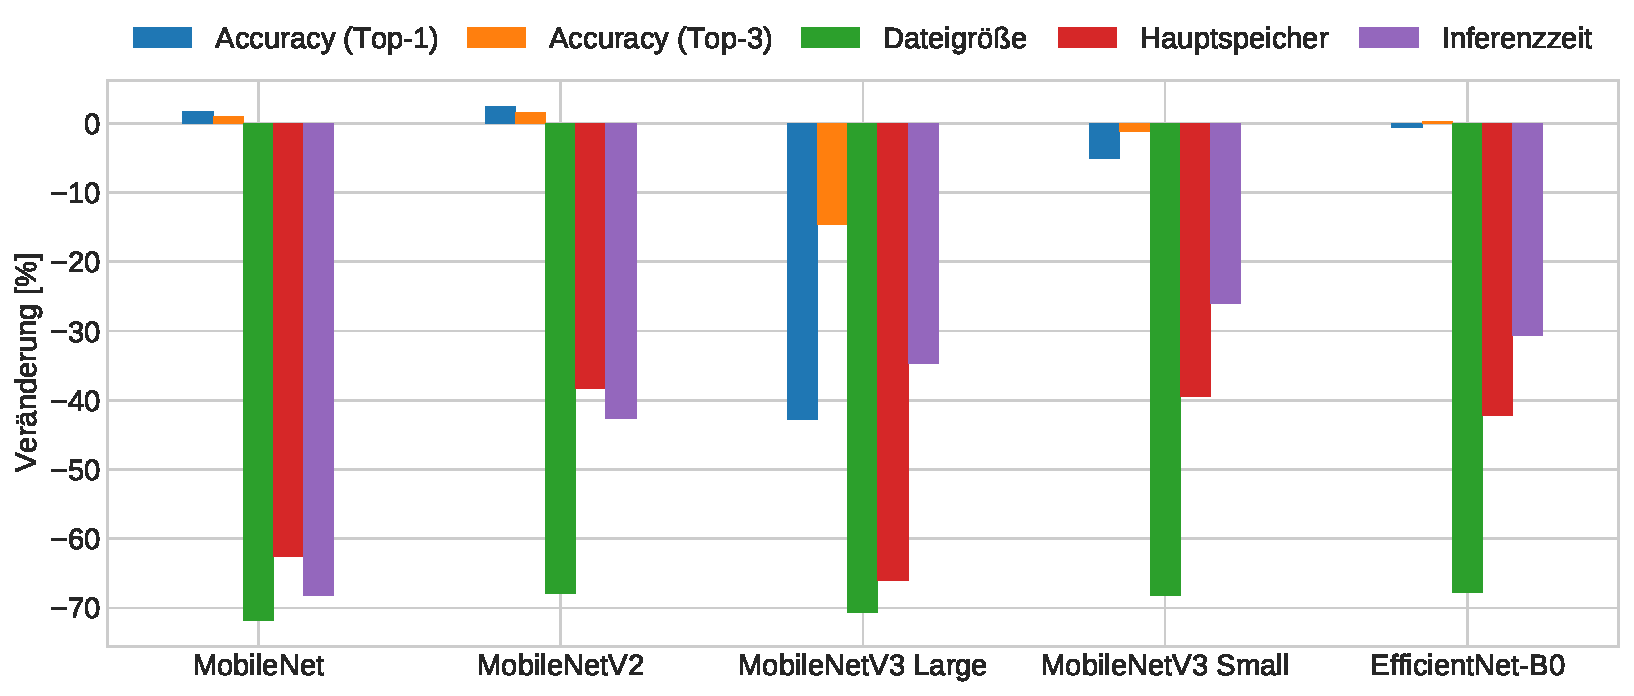
\includegraphics[width=\textwidth]{content/images/quantization_improvements.pdf}}
\caption{Prozentuale Veränderung der Metriken durch Anwendung von Quantisierung.}
\label{f4.1}
\end{figure}

Mit der Abbildung \ref{f4.1} wird sehr gut deutlich, wie sich die einzelnen Metriken bei der Anwendung von Quantisierung im Verhältnis zueinander verhalten und welche Kosten und welchen Nutzen eine Quantisierung dieser mobilen Architekturen beinhalten. Wie bereits am Anfang dieses Abschnittes diskutiert, lässt sich in Abbildung \ref{f4.1} erkennen, dass die Dateigröße der quantisierten Modelle gegenüber den nicht-quantisierten Modellen um ca. $70\%$ reduziert wird. Der Bedarf an Hauptspeicher und die Inferenzzeit werden je nach Architektur recht unterschiedlich beeinflusst. Es fällt jedoch auf, dass der Bedarf an Hauptspeicher bei der MobileNet und MobileNetV3 Large Architektur durch die Quantisierung um ungefähr $60\%$ reduziert werden kann. Die anderen Architekturen haben lediglich eine Reduktion von ungefähr $40\%$.

Bei der Diskussion der Auswirkung der Quantisierung auf die Genauigkeit am Anfang des Abschnittes wurde von einer Reduzierung der Genauigkeit ausgegangen. Jedoch zeigt Abbildung \ref{f4.1} und Tabelle \ref{t4.1}, dass die Genauigkeit nur sehr geringfügig beeinflusst wird. Tatsächlich verbessert sich sogar die Genauigkeit der MobileNet und MobileNetV2 Architektur um wenige Prozent. Die einzige Architektur, die bei der Quantisierung stark an Genauigkeit verloren hat, ist die MobileNetV3 Architektur. Die Top-1 Accuracy dieser Architektur ist durch die Quantisierung von $69.34\%$ auf $39.63\%$ abgefallen (siehe Tabelle \ref{t4.1}). Ein möglicher Grund für diesen Genauigkeitsverlust bei der Quantisierung der MobileNetV3 Large Architektur könnte sein, dass, wie im Abschnitt \ref{eval_training} bereits diskutiert, für das Training ungünstige Parameter gewählt wurden und somit diese Architektur schlecht trainiert ist. Durch dieses schlechte Training könnten möglicherweise einige Ausreißer in den Gewichten des Modells vorhanden sein, die für dieses schlechte Ergebnis bei der Quantisierung verantwortlich sind \cite{jacob_quantization_2017}. Damit eignet sich die MobileNetV3 Architektur bei dieser Trainingskonfiguration nicht für eine Post-Training Quantisierung.

Abgesehen von dem MobileNetV3 Large zeigen diese Ergebnisse, dass eine Post-Training Float Fallback Quantisierung der vorgestellten Architekturen mit wenig bis gar keinen Einbußen in der Genauigkeit durchgeführt werden kann. Jedoch sorgt diese Quantisierung für einen deutlich verringerten Bedarf an Hintergrundspeicher/Hauptspeicher und einer verringerten Inferenzzeit auf dem Raspberry Pi 4. Am meisten profitiert die MobileNet Architektur von der Quantisierung. Diese Architektur hat den Hintergrundspeicherbedarf, den Hauptspeicherbedarf und die Inferenzzeit um $62.6\%$ bis $71.9\%$ reduzieren können. Zusätzlich hat sich die Top-1 Accuracy um $1.7\%$ und die Top-3 Accuracy um $0.9\%$ gegenüber dem nicht quantisierten Modell verbessert.


\subsection{Pruning}
\label{eval_pruning}
Beim Pruning wird, wie bereits in Abschnitt \ref{impl_pruning} beschrieben, ein trainiertes Modell geladen und Schichten, die gepruned werden sollen, markiert. Anschließend werden, während eines erneuten Trainings auf dem bereits trainierten Modell, schrittweise Gewichte auf 0 gesetzt, die unter einen gewissen Schwellwert fallen. Nachdem dieses Vorgehen auf alle zu betrachteten Architekturen angewendet wurde, hat sich herausgestellt, dass der tatsächliche Anteil auf 0 gesetzter Gewichte (Sparsity) kleiner ist als der gewünschte Anteil. Der Grund dafür ist, dass TensorFlow beim Pruning den gewünschten Wert an Sparsity für jede markierte Schicht nur annähert. Zum anderen ist im Verlauf der Arbeit aufgefallen, dass in TensorFlow zum aktuellen Zeitpunkt zweidimensionale Depthwise Convolutions (\lstinline{tf.keras.layers.DepthwiseConv2D}) nicht gepruned werden. Das bedeutet, beim Markieren der \lstinline{DepthwiseConv2D} Schichten mittels der Funktion \lstinline{prune_layer}, wird die Schicht korrekt für das Pruning markiert. Jedoch werden im Verlauf des Pruningprozesses keine Gewichte dieser Schicht auf 0 gesetzt. Dieses Verhalten wurde zusätzlich in einem kleinen Minimalbeispiel verifiziert und Recherchen zu diesem Problem haben keine Lösung ergeben. Aus diesem Grund konnte das Problem in dieser Arbeit nicht behoben werden. Betrachtet man in Tabelle \ref{t4.4} die Anzahl an Parametern die durch die Depthwise Convolutions in die Architektur mit einfließen, kann man sehen, dass dies ein verhältnismäßig kleiner Anteil ist. Dieser kleine Anteil verringert aber trotzdem den Wert für die tatsächliche Sparsity.

\begin{table}[ht]
\centering
\begin{tabular}{llll}
\toprule
    Architekturen & Parameter & Parameter (Depthwise) & Anteil (Depthwise) \\
\midrule
        MobileNet &   3239114 &                 44640 &              1.38\% \\
      MobileNetV2 &   2270794 &                 64224 &              2.83\% \\
MobileNetV3 Large &   4239242 &                 91608 &              2.16\% \\
MobileNetV3 Small &   1540218 &                 58584 &              3.80\% \\
  EfficientNet-B0 &   4062381 &                182016 &              4.48\% \\
\bottomrule
\end{tabular}
\caption{Anteil an Parametern der Depthwise Convolutions zu der Gesamtparameterzahl der mobilen Architekturen.}
\label{t4.4}
\end{table}

Um sich der Frage nach den Auswirkungen von Pruning auf die mobilen Architekturen zu nähern, ist in Abbildung \ref{f4.2} die Top-1 Accuracy jeder Architektur für die verschiedenen exakten Sparsity-Werte nach dem Pruningvorgang dargestellt. Die $0\%$ Sparsity in der Abbildung \ref{f4.2} entsprechen den nicht geprunten Ausgangsmodellen nach dem erstmaligen Training. Wie in der Abbildung gut zu erkennen ist, verbessert sich bei allen Architekturen die Top-1 Accuracy, wenn die Architekturen auf $30\%$ Sparsity gepruned werden. Der Grund für die Verbesserung ist das erneute Training durch das Pruning und zusätzlich der geringe Anteil an Gewichten, die auf 0 gesetzt werden. Dadurch kann sich das Model leicht von den wenigen geprunten Gewichten erholen. Werden die Modelle auf $60\%$ gewünschte Sparsity gepruned, dann können das EfficientNet-B0 und das MobileNetV2 ihre ursprüngliche Genauigkeit ungefähr beibehalten. Das MobileNet und MobileNetV3 Large besitzen sogar bei $60\%$ Sparsity immer noch eine bessere Top-1 Accuracy als im nicht geprunten Zustand. Lediglich das MobileNetV3 Small hat sich leicht verschlechtert. Werden jedoch die Modelle auf $90\%$ gewünschte Sparsity gepruned, dann ergibt sich ein deutlich größerer Trade-Off. Alle Architekturen haben sich bei dieser Sparsity deutlich verschlechtert. Das MobileNetV3 Small verzeichnet nach diesem Pruningvorgang nur noch $46\%$ Top-1 Genauigkeit. Noch am besten hat dabei die MobileNet Architektur abgeschnitten, welche von einer Accuracy von $73\%$ auf eine Accuracy von $67\%$ abgefallen ist und damit bei einem Pruning mit $90\%$ gewünschter Sparsity von allen anderen betrachteten Architekturen die beste Genauigkeit aufweist.

\begin{figure}[htbp]
\centerline{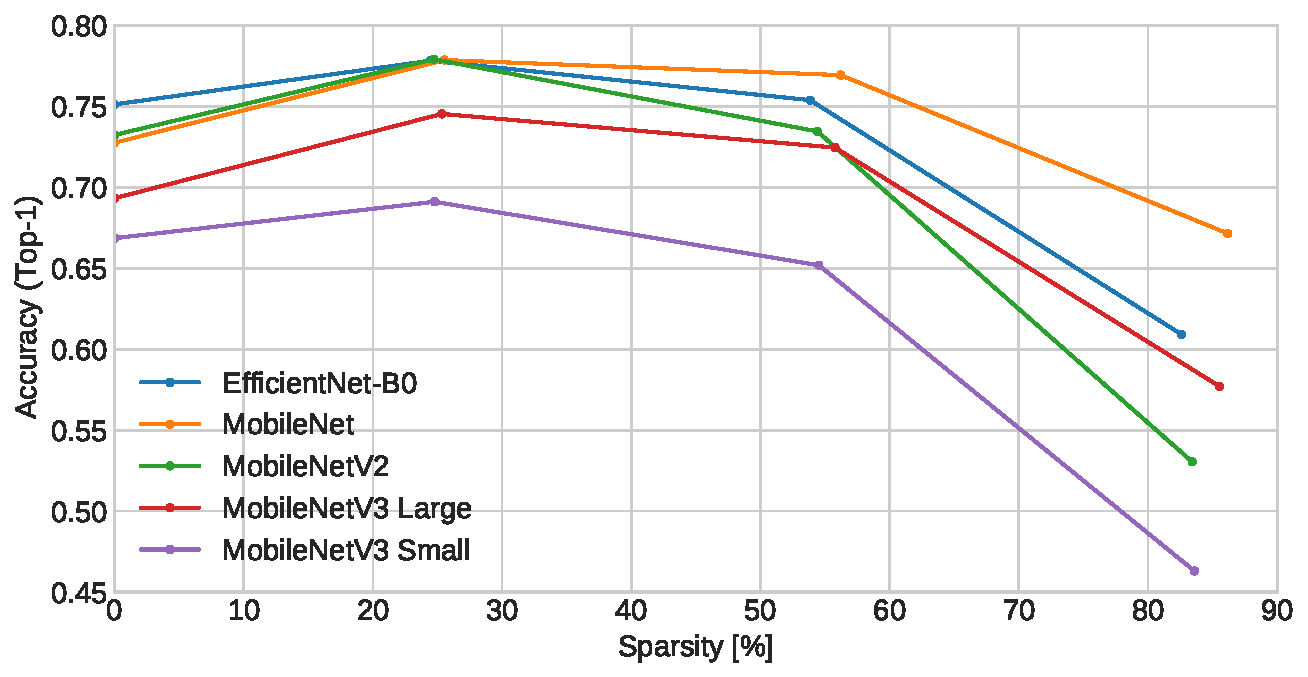
\includegraphics[width=0.8\textwidth]{content/images/sparsity_vs_accuracy.pdf}}
\caption{Genauigkeiten (Top-1) auf den Testdaten für die tatsächlichen Sparsity-Werte beim Pruning auf 0\% (ungepruned), 30\%, 60\% und 90\% Sparsity.}
\label{f4.2}
\end{figure}

Nach der Betrachtung der Genauigkeit stellt sich die Frage, welche Auswirkungen ein Pruning auf die restlichen betrachteten Metriken hat. Dazu ist in Tabelle \ref{t4.5} für jede Architektur und jede gewünschte Sparsity die tatsächliche Sparsity, der Hintergrundspeicherbedarf (Datei), der Bedarf an Hauptspeicher (RAM) und die Inferenzzeit aufgeführt. Was in dieser Tabelle sofort auffällt ist, dass die Metriken Hintergrundspeicherbedarf, Hauptspeicherbedarf und Inferenzzeit sich im Vergleich zu den nicht geprunten Ausgangsmodellen ($0\%$ Sparsity) in derselben Größenordnung befinden. Damit verbessert Pruning diese Metriken nicht.

Der Grund dafür, warum sich der Hauptspeicher- und Hintergrundspeicherbedarf nicht gegenüber den nicht-geprunten Modellen verändert, ist, dass beim Pruning die Gewichte nicht entfernt werden, sondern lediglich auf 0 gesetzt werden. Das bedeutet, bei einem 32 Bit Fließkomma-Modell (wie die trainierten Modelle in dieser Arbeit) werden beim Pruning die zu prunenden Gewichte auf die 32 Bit Fließkommazahl 0 gesetzt. Dadurch ergibt sich keine Speicherersparnis.

Zusätzlich wird in dieser Arbeit mit dem Magnitude Pruning ein unstrukturiertes Pruning betrieben, bei dem Gewichte an jeder beliebigen Stelle in dem Netzwerk gepruned werden können. Es wird beim unstrukturierten Pruning nicht darauf geachtet, die Gewichte in einer strukturierten Weise auf 0 zu setzen. Dies sorgt dafür, dass die aus dem unstrukturierten Pruning resultierenden Modelle nicht ohne weiteres bezüglich der Inferenzzeit optimiert werden können. Beim strukturierten Pruning hingegen werden ganze Neuronen, Filter oder Channel auf 0 gesetzt, was zu einer strukturierten Anordnung der geprunten Gewichten führt. Diese strukturiert geprunten Modelle können leichter durch Hardware und Software optimiert werden und können damit bessere Inferenzzeiten erreichen \cite{blalock_what_2020}.

\begin{table}[ht]
\centering
\begin{tabular}{llp{1.5cm}lll}
\toprule
Architekturen & Sparsity & Exakte Sparsity & Datei [MB] &  RAM [MB]  & Inferenz [µs]   \\
\midrule
MobileNet & 0\% &           0.00\% &     12.8453 &   16.1016 &          11803 \\
                & 30\% &          25.53\% &     12.8453 &   16.2148 &          11392 \\
                & 60\% &          56.21\% &     12.8453 &   16.1289 &          11594 \\
                & 90\% &          86.18\% &     12.8451 &   16.0625 &          11303 \\
\midrule
MobileNetV2 & 0\% &           0.00\% &      8.9153 &   11.2148 &           4961 \\
                & 30\% &          24.72\% &      8.9153 &   11.2656 &           4972 \\
                & 60\% &          54.41\% &      8.9153 &   11.2891 &           4933 \\
                & 90\% &          83.43\% &      8.9153 &   11.2617 &           4948 \\
\midrule
MobileNetV3 Large & 0\% &           0.00\% &     16.8829 &   20.4141 &           8051 \\
                & 30\% &          25.34\% &     16.8829 &   20.4180 &           7992 \\
                & 60\% &          55.78\% &     16.8829 &   20.3750 &           8098 \\
                & 90\% &          85.53\% &     16.8829 &   20.4727 &           8048 \\
\midrule
MobileNetV3 Small & 0\% &           0.00\% &      6.1536 &    8.5859 &           2954 \\
                & 30\% &          24.77\% &      6.1536 &    8.6211 &           2914 \\
                & 60\% &          54.52\% &      6.1536 &    8.6016 &           2959 \\
                & 90\% &          83.60\% &      6.1536 &    8.5898 &           2913 \\
\midrule
EfficientNet-B0 & 0\% &           0.00\% &     16.0860 &   16.6719 &          12453 \\
                & 30\% &          24.47\% &     16.0860 &   16.6484 &          12225 \\
                & 60\% &          53.86\% &     16.0860 &   16.5273 &          12376 \\
                & 90\% &          82.59\% &     16.0860 &   16.4492 &          12237 \\
\bottomrule
\end{tabular}
\caption{Zusammenfassung der exakten Sparsity, Dateigröße, Hauptspeicherbedarf und Inferenzzeit für die geprunten und unquantisierten Modelle.}
\label{t4.5}
\end{table}

Um aber trotzdem von den unstrukturiert geprunten Modellen zu profitieren, können die im \lstinline{.tflite}-Format gespeicherten Modelle mittels eines Kompressionsalgorithmus, wie gzip oder ZIP, komprimiert werden. Durch die hohe Anzahl an Gewichten mit dem Wert 0 sind diese Kompressionsalgorithmen in der Lage diese im TensorFlow Lite FlatBuffer gespeicherten Modelle stark zu komprimieren. Dieses Vorgehen wird so auch von dem Pruning-Guide \footnote{\url{https://www.tensorflow.org/model_optimization/guide/pruning/comprehensive_guide}} der TensorFlow Bibliothek vorgeschlagen. Abbildung \ref{f4.3} zeigt die Dateigröße der geprunten Modelle für jeden gewünschten Anteil an Sparsity nach Anwendung des gzip \footnote{\url{https://gzip.org/}} Kompressionsalgorithmus mit einem Kompressionslevel von 9. Der gzip Kompressionsalgorithmus wurde gewählt, da es sich um einen Algorithmus zum Komprimieren einzelner Dateien handelt und weil er in dem Pruning-Guide von TensorFlow als Beispiel verwendet wurde.

\begin{figure}[htbp]
\centerline{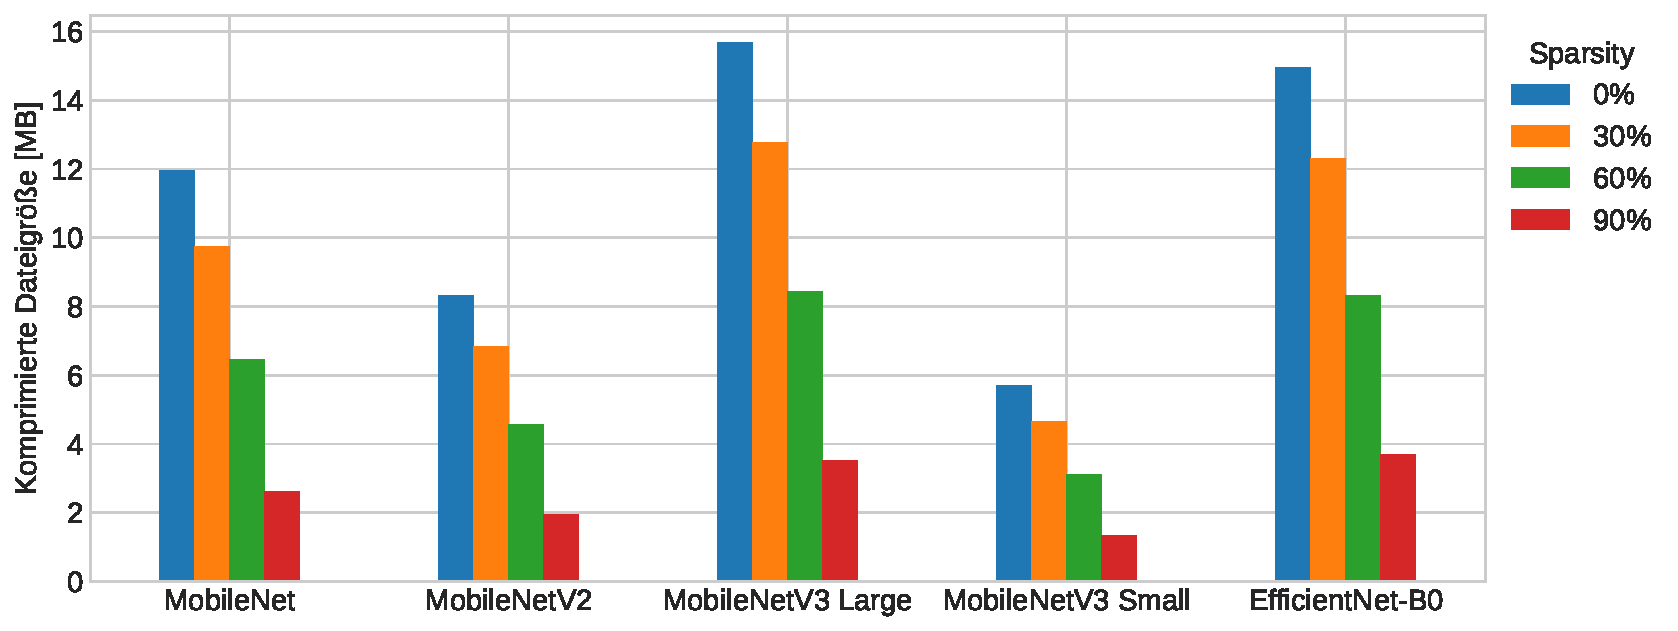
\includegraphics[width=\textwidth]{content/images/pruned_and_compressed.pdf}}
\caption{Dateigröße für Modelle mit $0\%$, $30\%$, $60\%$ und $90\%$ Sparsity nach Anwendung eines Kompressionsalgorithmus (gzip).}
\label{f4.3}
\end{figure}

Wie in Abbildung \ref{f4.3} gut zu ersehen ist, werden mit steigender Sparsity die komprimierten Modelle deutlich kleiner. So ist beispielsweise das MobileNet, welches ungepruned und komprimiert 12MB Hintergrundspeicher benötigt, nach Anwendung von Pruning mit einer gewünschten Sparsity von $90\%$ und Kompression nur noch 2.6MB groß. Die Speicherersparnis durch Kompression mit beispielsweise gzip hat den entscheidenden Nachteil, dass auf den komprimierten Modellen keine Inferenzen ausgeführt werden können. Um das Modell zu verwenden, muss die Kompression rückgängig gemacht werden und der volle Hintergrund- und Hauptspeicher für das Modell ohne Kompression wird benötigt. Jedoch ist in dem Fall, dass die Zielplattform, auf der die Inferenzen durchgeführt werden sollen, beispielsweise ein eingebettetes/verteiltes System ist, kann die Kombination aus Pruning und Kompression von entscheidendem Nutzen sein. Zum einen, wenn regelmäßig (z.B. als Update) trainierte Modelle über das Internet an eine entfernte Zielplattform gesendet werden sollen, oder aber auf der Zielplattform mit begrenzten Hintergrundspeicher sollen mehrere Modelle gespeichert werden, die aber nicht gleichzeitig verwendet werden. In diesen Fällen ist eine möglichst komprimierte Darstellung der Modelle hilfreich.


\subsection{Pruning und Quantisierung}
Bisher wurde betrachtet, was bei der Quantisierung und dem Pruning der vorgestellten Architekturen passiert. In diesem Abschnitt wird betrachtet, was passiert, wenn auf die vortrainierten Modelle als Erstes ein Pruning und anschließend eine Quantisierung angewendet wird.

Als Erstes ist in Abbildung \ref{f4.4} die Top-1 Genauigkeit der verschiedenen Modelle nach Anwendung von Pruning und Quantisierung dargestellt. Die ersten zwei Architekturen, die in dieser Grafik herausstechen, sind das MobileNetV3 Large und das EfficientNet-B0. Beim MobileNetV3 Large ist bei $0\%$ Sparsity erneut die schlechte Accuracy zu sehen, welche bereits in Abschnitt \ref{eval_quantisierung} diskutiert wurde. Durch das erneute Training während des Prunings hat sich die Genauigkeit des MobileNetV3 Large bei der Anwendung von Quantisierung verbessert. Zusätzlich fällt beim EfficientNet-B0 der Einbruch der Top-1 Accuracy beim Pruning mit einer gewünschten Sparsity von $30\%$ und anschließender Anwendung von Quantisierung auf. Dieser Einbruch der Genauigkeit hat sich beim Pruning auf eine gewünschte Sparsity von $60\%$ aber wieder ausgeglichen. Diese Ausreißer können möglicherweise durch ungünstig gewählte Parameter (Learning Rate Schedule, Pruning Schedule, Epochen, Batch Size, etc.) beim Training und Pruning der Architekturen entstehen. Am meisten profitieren die Architekturen MobileNet und MobileNetV2 von der Kombination aus Pruning und Quantisierung. Von beiden Architekturen ist die Top-1 Accuracy leicht besser, als wenn nur ein Pruning angewendet wird (siehe Abbildung \ref{f4.2}). Die restlichen Architekturen verhalten sich bezüglich der Top-1 Accuracy leicht schlechter als beim reinen Pruning ohne Anwendung von Quantisierung.

\begin{figure}[htbp]
\centerline{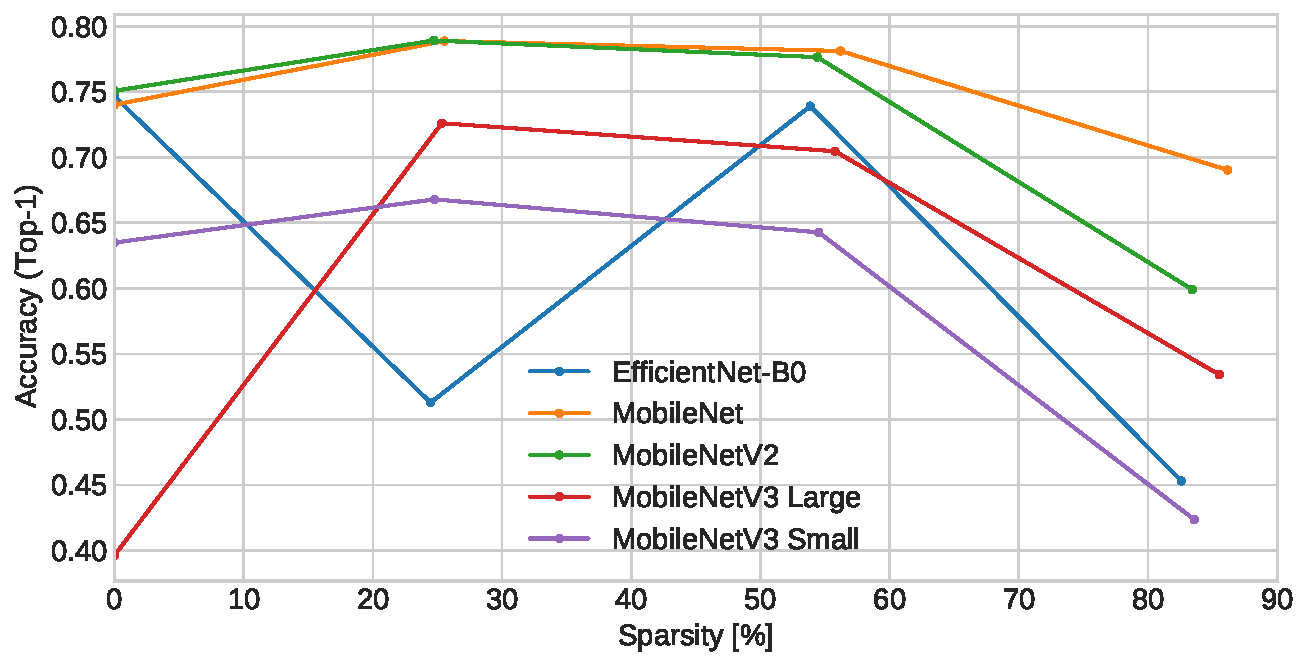
\includegraphics[width=0.8\textwidth]{content/images/sparsity_vs_accuracy_quantized.pdf}}
\caption{Genauigkeiten (Top-1) auf den Testdaten für die tatsächlichen Sparsity-Werte beim Pruning auf 0\% (ungepruned), 30\%, 60\% und 90\% Sparsity nach Anwendung von Quantisierung.}
\label{f4.4}
\end{figure}

Die Metriken Hintergrundspeicherbedarf, Hauptspeicherbedarf und Inferenzzeit sind für alle möglichen Sparsity Werte nahezu identisch und entsprechen den Werten für die quantisierten Modelle mit $0\%$ Sparsity in Tabelle \ref{t4.3}. Der Grund dafür wurde bereits in Abschnitt \ref{eval_pruning} diskutiert.

Besonders interessant wird die Kombination aus Pruning und Quantisierung, wenn diese Kombination nochmal mit einem Kompressionsalgorithmus wie gzip kombiniert wird. In Abschnitt \ref{eval_pruning} wurde bereits gezeigt, dass sich allein durch die Kombination von Pruning und einem Kompressionsalgorithmus die Größe der Modelle deutlich reduzieren lässt. Werden nun die geprunten Modelle vor der Kompression mit gzip noch quantisiert, dann ergeben sich für die einzelnen Architekturen die in Abbildung \ref{f4.5} dargestellten Dateigrößen.

\begin{figure}[htbp]
\centerline{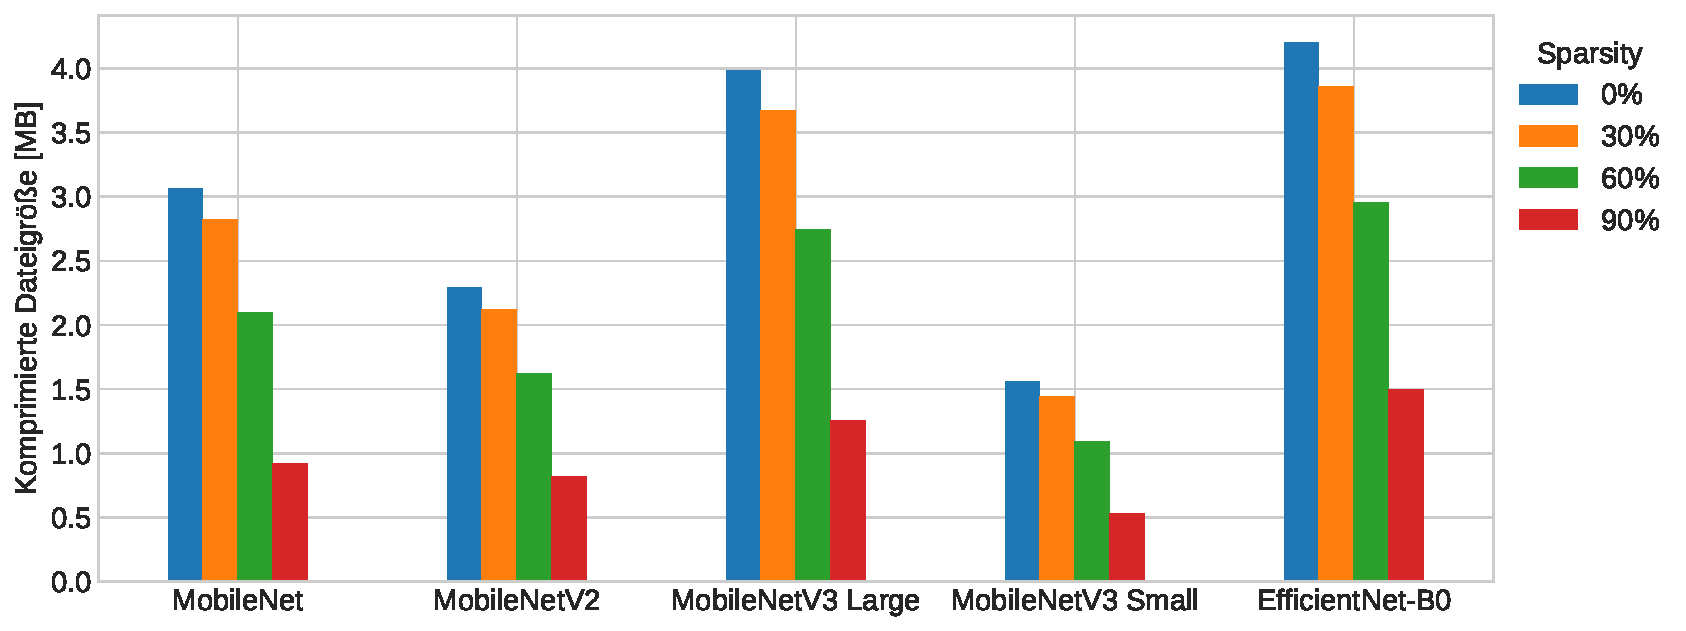
\includegraphics[width=\textwidth]{content/images/pruned_and_compressed_quantized.pdf}}
\caption{Dateigröße für Modelle mit $0\%$, $30\%$, $60\%$ und $90\%$ Sparsity nach Anwendung von Quantisierung und eines Kompressionsalgorithmus (gzip).}
\label{f4.5}
\end{figure}

Verglichen mit den Dateigrößen in Abbildung \ref{f4.3} hat die Quantisierung der Modelle vor der Kompression die Dateigröße nochmal deutlich reduziert. Beispielsweise hat das MobileNet nach der Anwendung von Pruning ($90\%$ Sparsity), Quantisierung und Kompression mittels gzip nur noch einen Hintergrundspeicherbedarf von 0.9MB. Verglichen mit dem komprimierten MobileNet ohne Anwendung von Pruning und Quantisierung mit 12MB Hintergrundspeicherbedarf ist das eine Reduktion um das 13-fache.

Das kleinste Modell nach Anwendung von Pruning ($90\%$ Sparsity), Quantisierung und Kompression ist das MobileNetV3 Small mit 0.5MB Hintergrundspeicherbedarf.


\section{Einfluss der Optimierungen auf die Klassen}
Der folgende Abschnitt stellt eine weitere Evaluationsmetrik vor, welche angelehnt ist an das Paper "What Do Compressed Deep Neural Networks Forget?" von Sara Hooker et al. \cite{hooker_what_2020}.

Um die Architekturen untereinander zu vergleichen und die Auswirkungen von Quantisierung und Pruning auf die vorgestellten Architekturen zu bewerten, wurden in dieser Arbeit bisher unter anderem die Top-1 und Top-3 Genauigkeit verwendet. Diese Top-1 und Top-3 Genauigkeit gibt das Verhältnis zwischen der Anzahl der korrekt klassifizierten Beispiele zu der Anzahl aller Beispiele an. Bisher wurde in dieser Arbeit diese Genauigkeit unabhängig von der Klassenzugehörigkeit der jeweiligen Beispiele bestimmt. Jedoch lässt sich die Genauigkeit auch für jede einzelne Klasse bestimmen, indem die Anzahl der korrekt klassifizierten Beispiele einer Klasse zu der Anzahl aller Beispiele einer Klasse für alle Klassen ins Verhältnis gesetzt wird. Wird angenommen, dass sich der Verlust durch die Optimierungstechniken gleichmäßig auf die Genauigkeit der einzelnen Klassen auswirkt, dann würde sich das Modell nach Anwendung der Optimierungen noch annähernd gleich verhalten. Es wurde jedoch gezeigt, dass Pruning und Quantisierung die Genauigkeit der einzelnen Klassen eines Modells unterschiedlich stark beeinflussen \cite{hooker_what_2020}. Dies kann beispielsweise zur Folge haben, dass eine Klasse durch die Anwendung von Pruning deutlich an Genauigkeit verliert, während die anderen Klassen nur leicht an Genauigkeit verlieren. Der ungleichmäßige Genauigkeitsverlust kann in einigen Anwendungsbereichen, wie bei selbstfahrenden Autos oder in der Medizintechnik, katastrophale Folgen haben. Aus diesem Grund sollte nicht allein auf die generelle Genauigkeit vertraut werden, sondern auch für jede Klasse separat die Genauigkeit betrachtet werden. 

\begin{table}[ht]
\centering
\begin{tabular}{l|llll|llll}
\toprule
               & \multicolumn{4}{c}{MobileNet}           & \multicolumn{4}{c}{EfficientNet-B0} \\
               &       0\% &   30\% &   60\% &    Quant. &    0\% &   30\% &   60\%   & Quant. \\
\midrule
Automobil      &     0.738 &  0.862 &  0.844 &     0.732 &    0.792 &  0.870 &  0.873 &     0.771 \\
Flugzeug       &     0.697 &  0.835 &  0.836 &     0.689 &    0.847 &  0.817 &  0.789 &     0.817 \\
Frosch         &     0.786 &  0.845 &  0.830 &     0.806 &    0.825 &  0.835 &  0.818 &     0.824 \\
Hirsch         &     0.724 &  0.764 &  0.755 &     0.715 &    0.785 &  0.752 &  0.717 &     0.780 \\
Hund           &     0.665 &  0.642 &  0.620 &     0.666 &    0.575 &  0.601 &  0.580 &     0.552 \\
Katze          &     0.441 &  0.602 &  0.627 &     0.416 &    0.521 &  0.655 &  0.628 &     0.542 \\
LKW &     0.917 &  0.861 &  0.849 &     0.922 &    0.894 &  0.854 &  0.829 &     0.895 \\
Pferd          &     0.761 &  0.838 &  0.820 &     0.768 &    0.844 &  0.802 &  0.776 &     0.833 \\
Schiff         &     0.841 &  0.860 &  0.860 &     0.844 &    0.898 &  0.879 &  0.855 &     0.886 \\
Vogel          &     0.707 &  0.679 &  0.654 &     0.690 &    0.533 &  0.705 &  0.675 &     0.447 \\
\bottomrule
\end{tabular}
\caption{Klassenweise Top-1 Accuracy der MobileNet und EfficientNet-B0 Architekturen auf dem CIFAR-10 Datensatz für die Modelle mit $0\%$, $30\%$, $60\%$ und $90\%$ Sparsity und dem ungeprunten quantisierten Modellen (Quant.).}
\label{t4.6}
\end{table}

Im Folgenden wird exemplarisch an der MobileNet und EfficientNet-B0 Architektur betrachtet, wie sich ein Pruning mit $30\%$, $60\%$ und $90\%$ Sparsity und eine Quantisierung der ungeprunten Modelle auf die einzelnen Klassen auswirkt. Dazu sind in Tabelle \ref{t4.6} die Top-1 Genauigkeiten auf den Testdaten für jede der 10 Klassen des CIFAR-10 Datensatzes dargestellt. Was in der Tabelle \ref{t4.6} direkt auffällt ist, dass die Genauigkeiten jeder Klasse sehr unterschiedlich sein können. Beispielsweise ist beim nicht geprunten MobileNet die Genauigkeit für die Klasse Katze $44.1\%$ während die Klasse LKW eine Genauigkeit von $91.7\%$ besitzt. Damit scheint das in dieser Arbeit trainierte MobileNet besser dazu in der Lage zu sein LKWs zu klassifizieren als Katzen.

Um nun zu visualisieren, wie sich die Genauigkeit der einzelnen Modelle während des Prunings und der Quantisierung im Vergleich zum Ausgangsmodell mit $0\%$ Sparsity verändert hat, wurde für jede Klasse die Differenz zwischen dem optimierten Modell und dem Ausgangsmodell gebildet.

Abbildung \ref{f4.6} zeigt die Veränderung der Genauigkeit in Prozentpunkten für die MobileNet Architektur beim Pruning mit den verschiedenen gewünschten Sparsity-Werten. Würde sich die Veränderung der Genauigkeit durch die Anwendung von Pruning gleichermaßen auf alle Klassen auswirken, müssten alle Balken in dem Balkendiagramm die gleiche Länge und Ausrichtung haben. Jedoch ist sehr gut ersichtlich, wie unterschiedlich die Veränderung durch das Pruning ist. Beispielsweise hat sich während des Prunings auf $30\%$ Sparsity die Klasse Katze um $16.1\%$-Punkte verbessert, während sich die Klasse LKW um $5.6\%$-Punkte verschlechtert hat. Wird das MobileNet auf $90\%$ Sparsity gepruned lässt sich gut erkennen, wie die Klasse Vogel um $19.8\%$-Punkte Genauigkeit verliert. Das ist ein gutes Beispiel dafür, dass es wichtig ist die Genauigkeiten der einzelnen Klassen im Blick zu haben, da die MobileNet Architektur beim Pruning auf $90\%$ Sparsity lediglich $6\%$-Punkte an Genauigkeit verloren hat (siehe Abschnitt \ref{eval_pruning}), jedoch hat die Klasse Vogel $19.8\%$-Punkte Genauigkeit eingebüßt. Wenn die Anwendung aber Wert darauf legt, dass Vögel korrekt klassifiziert werden, kann die Betrachtung der generellen Top-1 Accuracy über alle Klassen täuschen.

\begin{figure}[htbp]
\centerline{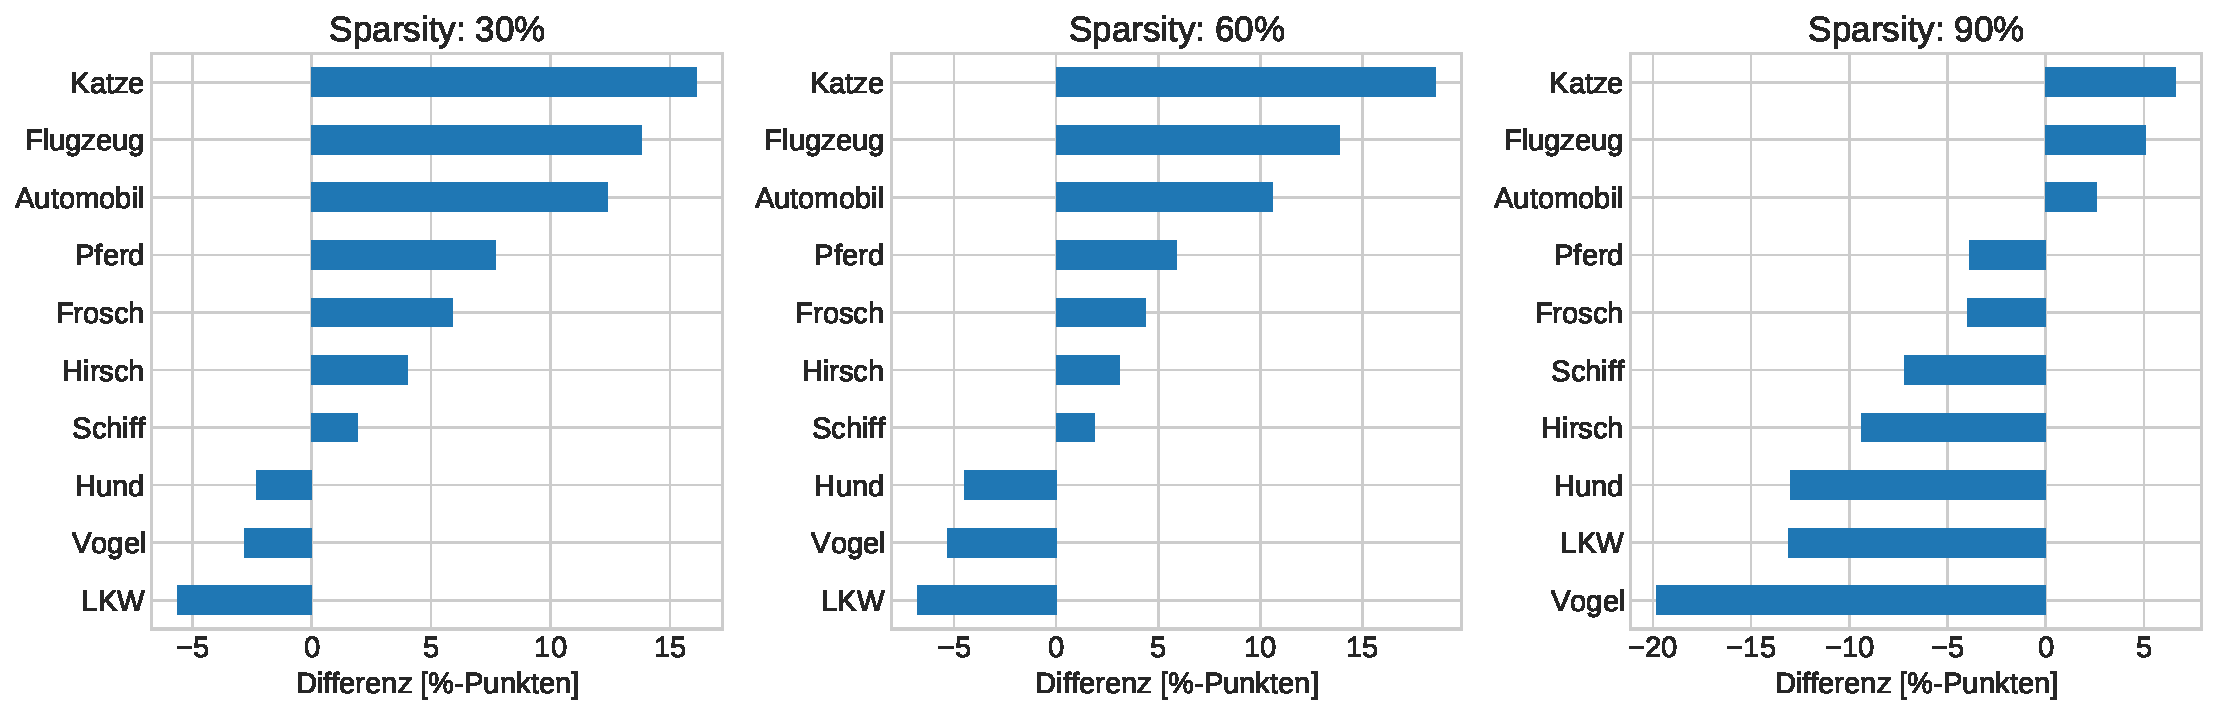
\includegraphics[width=\textwidth]{content/images/classwise_acc_change_pruning_mobilenet.pdf}}
\caption{Veränderung der klassenweisen Top-1 Genauigkeit der geprunten MobileNet Modelle mit $30\%$, $60\%$ und $90\%$ Sparsity in Prozentpunkten.}
\label{f4.6}
\end{figure}

In Abbildung \ref{f4.7} ist die klassenweise Veränderung der EfficientNet-B0 Architektur für die verschiedenen Sparsity-Werte dargestellt. Wie auch hier zu sehen ist, beeinflusst das Pruning die Genauigkeit der einzelnen Klassen sehr unterschiedlich. Am meisten profitieren die Klassen Vogel, Katze und Automobil vom Pruning der EfficientNet-B0 Architektur. Wie in Abbildung \ref{f4.2} ersichtlich, verliert die EfficientNet-B0 Architektur im Verlauf des Prunings auf $90\%$ gewünschte Sparsity insgesamt $14\%$-Punkte an Top-1 Genauigkeit. Das ist deutlich mehr Verlust als beim MobileNet während des Prunings. Dies spiegelt sich auch in der klassenweisen Genauigkeit in Abbildung \ref{f4.7} wieder. Bei $90\%$ Sparsity haben alle Klassen an Genauigkeit verloren. Die Klassen LKW, Flugzeug und Hirsch haben dabei mit über $20\%$-Punkten den größten Verlust an Top-1 Genauigkeit.

\begin{figure}[htbp]
\centerline{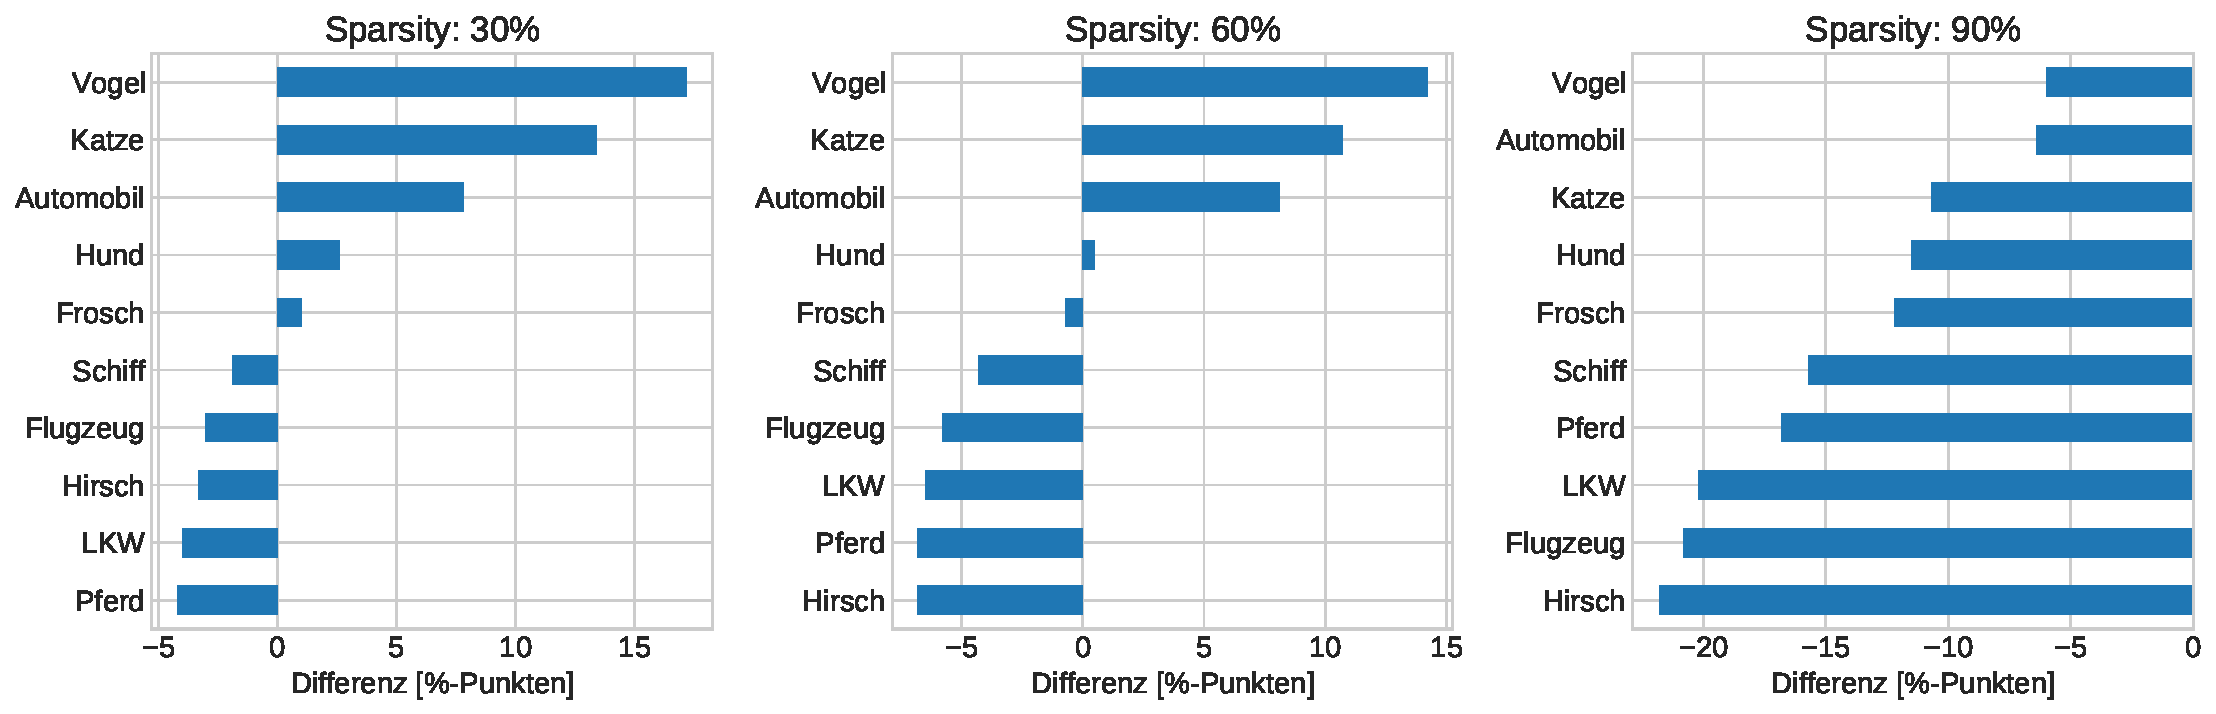
\includegraphics[width=\textwidth]{content/images/classwise_acc_change_pruning_efficientnet-b0.pdf}}
\caption{Veränderung der klassenweisen Top-1 Genauigkeit der geprunten EfficientNet-B0 Modelle mit $30\%$, $60\%$ und $90\%$ Sparsity in Prozentpunkten.}
\label{f4.7}
\end{figure}

Nachdem nun der klassenweise Verlust bei der Anwendung von Pruning auf die zwei exemplarischen Architekturen MobileNet und EfficientNet-B0 diskutiert wurde, stellt sich noch die Frage, wie sich die Post-Training Quantisierung auf die Genauigkeit der einzelnen Klassen auswirkt. Dazu stellt Abbildung \ref{f4.8} die Veränderungen der klassenweisen Top-1 Genauigkeiten der MobileNet und EfficientNet-B0 Architekturen dar.

\begin{figure}[htbp]
\centerline{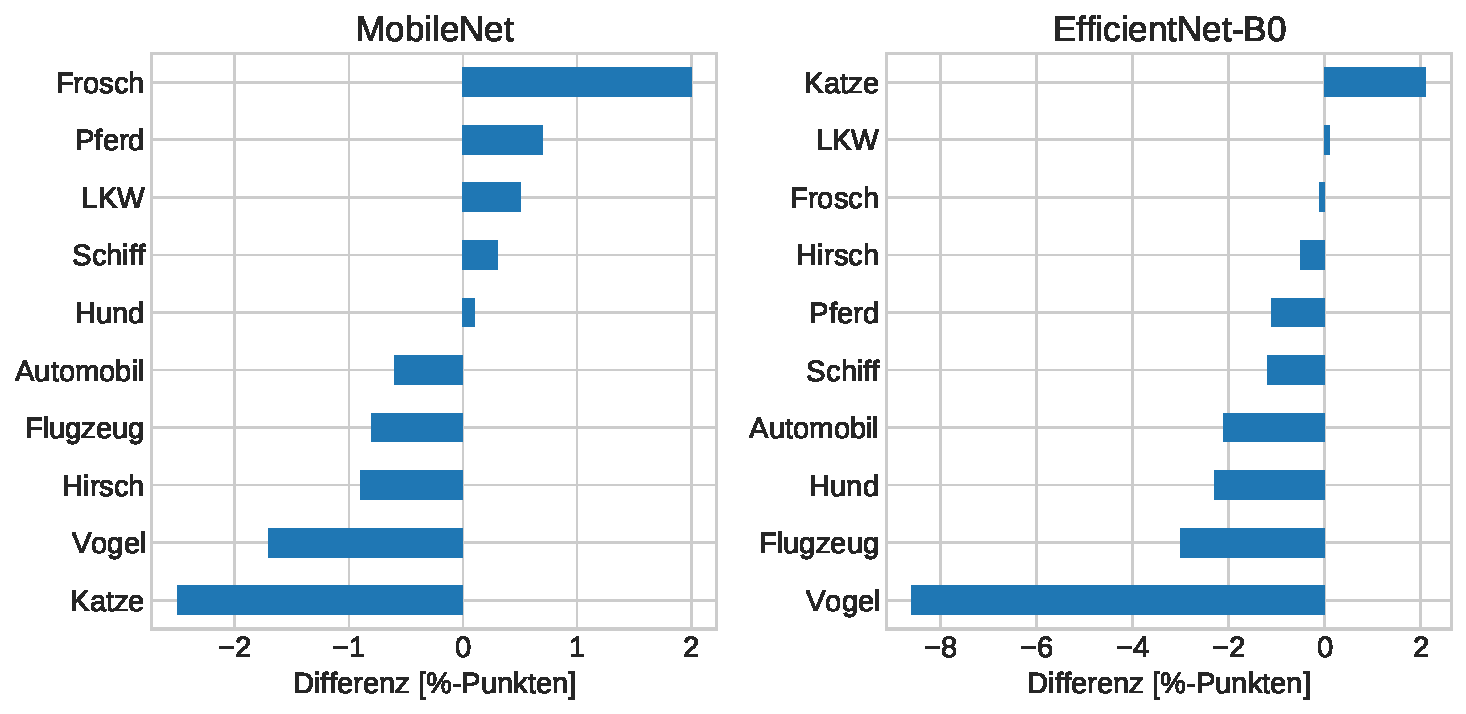
\includegraphics[width=0.7\textwidth]{content/images/classwise_acc_change_quantization.pdf}}
\caption{Differenz der klassenweisen Top-1 Accuracy des nicht quantisierten MobileNet Modells und des quantisierten MobileNet Modells.}
\label{f4.8}
\end{figure}

Genau wie beim Pruning ist bei der Quantisierung ebenfalls deutlich zu erkennen, dass die Anwendung dieser Optimierungstechnik zu einer ungleichmäßigen Veränderung der Genauigkeiten der einzelnen Klassen geführt hat. Am wenigsten hat die Quantisierung die Genauigkeiten der einzelnen Klassen bei der MobileNet Architektur beeinflusst. Bei dieser Architektur hat die Klasse Frosch mit $2\%$-Punkten verbesserter Genauigkeit am stärksten von der Quantisierung profitiert. Die Klasse Katze hat mit $2.5\%$-Punkten den größten Verlust durch die Quantisierung zu verzeichnen. Bei der EfficientNet-B0 Architektur wurde die Genauigkeit der einzelnen Klassen deutlich stärker von der Quantisierung beeinflusst als beim MobileNet. Beim EfficientNet-B0 profitiert die Klasse Katze mit $2.1\%$-Punkte von der Quantisierung am meisten. Die Klasse Vogel ist beim quantisierten EfficientNet-B0 erneut ein gutes Beispiel dafür, warum die Betrachtung der klassenweisen Genauigkeit besonders wichtig ist. Die Klasse Vogel hat beim Quantisieren der Architektur $8.6\%$-Punkte an Genauigkeit verloren, während der Verlust an Genauigkeit der anderen Klassen recht begrenzt ist. Angenommen die Klasse Vogel ist für den Anwendungsbereich, in der das Modell eingesetzt werden soll, von besonderer Bedeutung, kann dieser enorme Genauigkeitsverlust zu Problemen führen. Insgesamt verliert die EfficientNet-B0 Architektur durch die Anwendung von Quantisierung nur $0.5\%$-Punkte an Top-1 Genauigkeit (siehe Abschnitt \ref{eval_training} und Abschnitt \ref{eval_quantisierung}). Daran lässt sich gut erkennen, dass die generelle Genauigkeit über alle Klassen wichtige Veränderungen für einzelne Klassen verschleiert.



\section{Optimierungen}
Bisher wurden in dieser Arbeit ausschließlich die unveränderten Standardvarianten der Architekturen MobileNet, MobileNetV2, MobileNetV3 und EfficientNet vorgestellt und untersucht. Diese Architekturen haben sich zum Ziel gesetzt, besonders wenig Ressourcen zu benötigen, um in einem mobilen oder eingebetteten System Anwendung zu finden. Durch Optimierungstechniken wie Quantisierung und Pruning lässt sich der Ressourcenbedarf dieser Architekturen drastisch reduzieren (siehe Abschnitt \ref{ergebnisse}). Dies geht aber oft auf Kosten einer verminderten Genauigkeit der trainierten und optimierten Modelle. Zusätzlich werden in den vorgestellten Architekturen teilweise Schichten verwendet, die noch nicht so gut von Hardware oder Software unterstützt werden. Dies kann beispielsweise zu einer erhöhten Inferenzzeit führen. In diesem Abschnitt soll untersucht und diskutiert werden, was für Optimierungen durchgeführt werden können, um die vorgestellten Architekturen weiter zu optimieren.

Bereits im Abschnitt \ref{eval_training} wurde diskutiert, dass der exzessive Gebrauch von Squeeze-And-Excitation Modulen zu einer erhöhten Inferenzzeit auf dem Raspberry Pi 4 führt. Dies ist vermutlich auch der Grund dafür, warum die EfficientNet-B0 Architektur eine um $54.7\%$ erhöhte Inferenzzeit im Vergleich zu der ähnlich großen MobileNetV3 Large Architektur besitzt. Die EfficientNet-B0 Architektur ist architekturell recht ähnlich zu der MobileNetV3 Large Architektur, jedoch verwendet sie $50\%$ mehr Squeeze-And-Excitation Module als die MobileNetV3 Large Architektur.

Um mitunter das Problem mit den Squeeze-And-Excitation Modulen zu beheben, wurden die in Abschnitt \ref{efficientnet} beschriebenen EfficientNet-lite Architekturen veröffentlicht \cite{liu_higher_2020}. Diese EfficientNet-lite Architekturen haben eine Reihe an architekturellen Optimierungen vorgenommen, welche eine breitere Hardwarekompatibilität, weniger Parameter und bessere Quantisierbarkeit erreichen sollen. Die vorgenommenen Optimierungen sind \cite{liu_higher_2020}:
\begin{itemize}
\item Squeeze-And-Excitation Module wurden entfernt, um eine bessere und breitere Hardwarekompatibilität zu ermöglichen.
\item Die Swish Aktivierungsfunktion wurde durch die ReLU6 Aktivierungsfunktion ersetzt, um eine bessere Quantisierbarkeit mittels Post-Training Quantization zu erreichen.
\item Um die Größe der Architektur und die Anzahl an Berechnungen zu verringern, wurden einige Parameter vom Compound Scaling ausgeschlossen.
\end{itemize}
Das Problem mit diesen EfficientNet-lite Architekturen ist, dass zum Zeitpunkt, zu dem diese Arbeit entstanden ist, noch kein Paper zu diesen Architekturen veröffentlicht wurde. Es existierte lediglich ein Blog-Post von TensorFlow, welcher grob die Optimierungen dieser Architekturen beschreibt \cite{liu_higher_2020}. Von TensorFlow gibt es zwar auf dem ImageNet Datensatz vortrainierte EfficientNet-lite Modelle \footnote{\url{https://tfhub.dev/s?q=EfficientNet-Lite}}, jedoch ist es nicht gelungen das in dieser Arbeit verwendete Evaluationsverfahren auf diese Architekturen anzuwenden. 

Eine weitere Architektur, zu der eine optimierte Variante existiert, ist die MobileNetV3 Large/Small Architektur. TensorFlow bietet für diese beiden Architekturen jeweils eine so genannte Minimalistic-Variante \footnote{\url{https://www.tensorflow.org/api_docs/python/tf/keras/applications/MobileNetV3Large}} \footnote{\url{https://www.tensorflow.org/api_docs/python/tf/keras/applications/MobileNetV3Small}} an, welche teilweise recht ähnliche Optimierungen vornimmt wie die EfficientNet-lite Architekturen. Diese Optimierungen sind:
\begin{itemize}
\item Ebenfalls wie bei den EfficientNet-lite Architekturen wurden die Squeeze-And-Excitation Module entfernt.
\item Die Hard-Swish Aktivierungsfunktion wurde durch die ReLU Aktivierungsfunktion ersetzt.
\item Außerdem wurden Convolutions mit einer Kernelgröße von $5 \times 5$ durch Convolutions mit einer Kernelgröße von $3 \times 3$ ausgetauscht.
\end{itemize}
Ansonsten entsprechen die MobileNetV3 Minimalistic Architekturen vom Aufbau den normalen MobileNetV3 Architekturen. Zusätzlich sind die MobileNetV3 Minimalistic Architekturen sehr gut in der TensorFlow Bibliothek implementiert und lassen sich genauso wie die anderen vorgestellten Architekturen verwenden.

Im Folgenden wird anhand der MobileNetV3 Minimalistic Architekturen untersucht, inwieweit sich die architekturellen Optimierungen auf die MobileNetV3 Architektur auswirken und wie sich die MobileNetV3 Minimalistic Architekturen unter Anwendung von Quantisierung und Pruning verhalten.

Dazu werden die MobileNetV3 Large/Small Minimalistic Architekturen zuerst auf dem CIFAR-10 Datensatz trainiert und anschließend analog zu den anderen Architekturen evaluiert. Bei dem Training und beim Pruning musste von dem einheitlichen Setup für alle Experimente (siehe Abschnitt \ref{training} und Abschnitt \ref{impl_pruning}) leicht abgewichen werden. Das bedeutet, dass die initiale und schlussendliche Learning Rate beim Training und Pruning um den Faktor $10^{-1}$ reduziert wurde. Der Grund dafür ist, dass ansonsten der Loss der MobileNetV3 Minimalistic Architekturen während des Trainings dazu tendiert zu divergieren. Nach dem Training der MobileNetV3 Minimalistic Architekturen ergeben sich folgende Kennwerte, welche in Tabelle \ref{t4.7} dargestellt sind.

\begin{table}[ht]
\centering
\begin{tabular}{lllllll}
\toprule
 & Parameter &  Top-1 &  Top-3 &  Datei [MB] &  RAM [MB] &  Inferenz [µs] \\
\midrule
            Large &  2.7 Mio. & 0.6949 & 0.9128 &     10.6120 &   14.2344 &        5297 \\
            Small &  1.0 Mio. & 0.6099 & 0.8755 &      4.1234 &    6.1797 &        1826 \\
\bottomrule
\end{tabular}
\caption{Kennwerte der MobileNetV3 Large/Small Minimalistic Modelle nach dem Training auf dem CIFAR-10 Datensatz. Top-1/Top-3 entsprechen der Top-1/Top-3 Genauigkeit auf den Testdaten.}
\label{t4.7}
\end{table}

Wird die Tabelle \ref{t4.7} mit der Tabelle \ref{t4.1} und Tabelle \ref{t4.2} verglichen, fällt zum einen auf, dass die Parameterzahl der MobileNetV3 Minimalistic Modelle um einiges geringer ist als bei den normalen MobileNetV3 Architekturen. Dies ergibt sich daraus, dass die Squeeze-And-Excitation Module entfernt wurden und die $5 \times 5$ Convolutions durch $3 \times 3$ Convolutions ersetzt wurden. Dies sorgt beides für eine verringerte Parameterzahl der Architekturen. Zum anderen fällt auf, dass die Inferenzzeit beider Minimalistic Architekturen gesunken ist. Dies ist vermutlich bedingt durch die verringerte Parameterzahl und durch das Entfernen der schlecht unterstützten Squeeze-And-Excitation Module. Weiter kann man in Tabelle \ref{t4.7} erkennen, dass die Genauigkeit des MobileNetV3 Large Minimalistic nahezu gleich geblieben ist zu der Genauigkeit des normalen MobileNetV3 Large. Das MobileNetV3 Small Minimalistic hat leicht an Genauigkeit verloren. Die Dateigröße der Modelle und der Bedarf an Hauptspeicher ist ebenfalls stark gesunken, was durch die gesunkene Parameterzahl bedingt ist.

Werden nun diese Modelle mittels Post-Training Float-Fallback Quantisierung quantisiert, ergeben sich die in Tabelle \ref{t4.8} beschriebenen Kennwerte für die Modelle. In dieser Tabelle lässt sich gut erkennen, dass sich durch die Quantisierung die Größe und Inferenzzeit der Modelle drastisch reduziert hat. Nach der Quantisierung benötigt das MobileNetV3 Small Minimalistic auf dem Raspberry Pi 4 nur noch 1.1ms für die Inferenz eines Eingabebildes.

\begin{table}[ht]
\centering
\begin{tabular}{lllllll}
\toprule
 & Parameter &  Top-1 &  Top-3 &  Datei [MB] &  RAM [MB] &  Inferenz [µs] \\
\midrule
            Large &  2.7 Mio. & 0.7050 & 0.9269 &      3.1612 &   5.57420 &        2839 \\
            Small &  1.0 Mio. & 0.6343 & 0.8879 &      1.3065 &   4.37891 &        1118 \\
\bottomrule
\end{tabular}
\caption{Kennwerte der trainierten und quantisierten MobileNetV3 Large/Small Minimalistic Modelle.}
\label{t4.8}
\end{table}

Um die Veränderung durch die Quantisierung im Verhältnis zu den nicht quantisierten Modellen besser zu visualisieren, wird in Abbildung \ref{f4.9} genau wie in Abschnitt \ref{eval_quantisierung} die prozentuale Veränderung der einzelnen Metriken für jedes Modell in Bezug auf die nicht quantisierten Modelle dargestellt. Dabei werden zusätzlich neben den Minimalistic-Varianten der MobileNetV3 Architektur auch die quantisierten MobileNetV3 Large/Small Architekturen dargestellt.

\begin{figure}[htbp]
\centerline{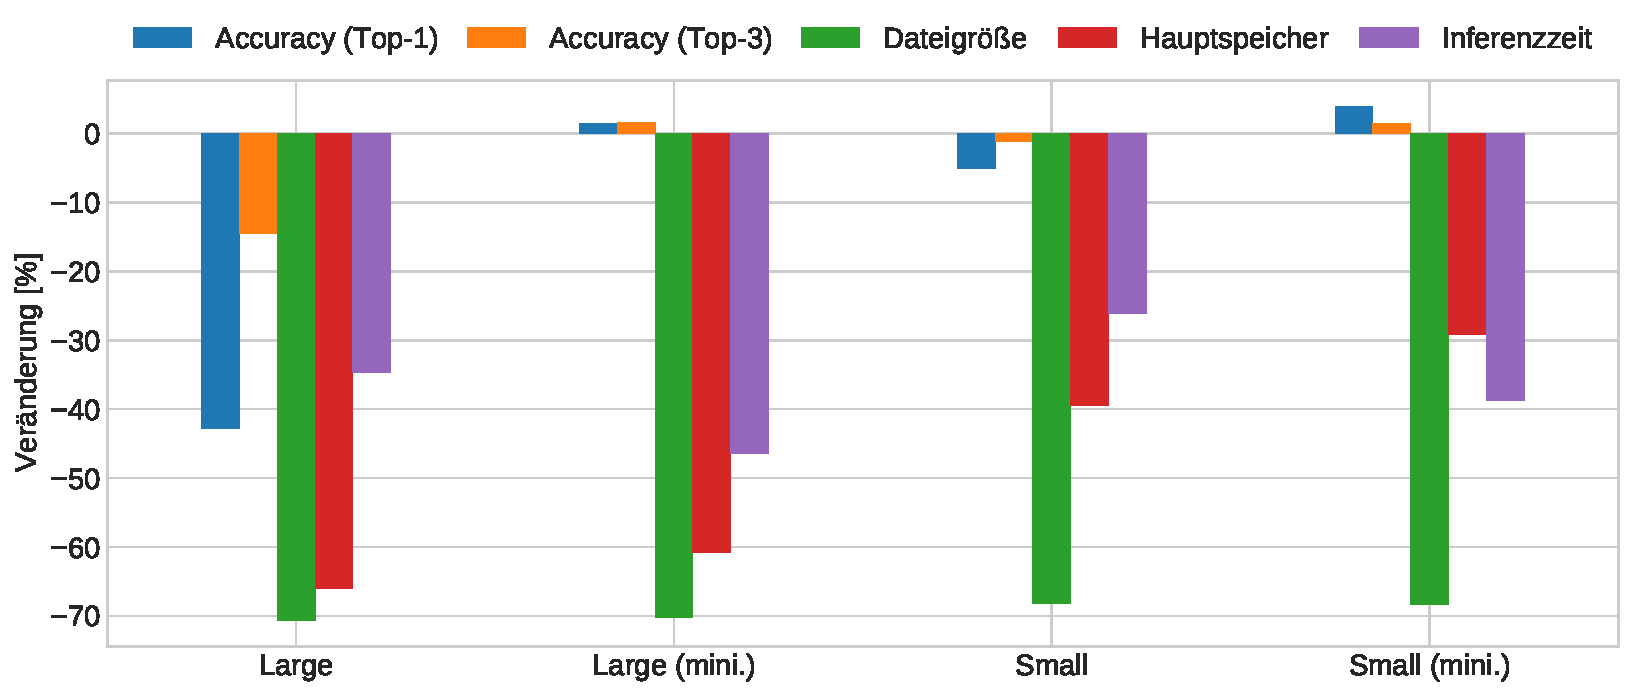
\includegraphics[width=0.9\textwidth]{content/images/quantization_improvements_mnv3mini.pdf}}
\caption{Prozentuale Veränderung der Metriken der MobileNetV3 Varianten durch Anwendung von Quantisierung.}
\label{f4.9}
\end{figure}

Die Abbildung \ref{f4.9} zeigt, wie die MobileNetV3 Minimalistic Architektur bei der Quantisierung durch die architekturellen Optimierungen profitiert. Während beide MobileNetV3 Architekturen durch die Quantisierung an Genauigkeit verlieren, gewinnen die beiden MobileNetV3 Minimalistic an Genauigkeit. Selbst das MobileNetV3 Large Minimalistic gewinnt leicht an Genauigkeit, obwohl sich das normale MobileNetV3 Large am stärksten von allen betrachteten Architekturen durch die Quantisierung verschlechtert hat. Zusätzlich fällt auf, dass sich bei allen Minimalistic-Varianten die Inferenzzeit durch die Quantisierung stärker hat reduzieren lassen als bei den normalen MobileNetV3 Architekturen. Dies kann möglicherweise mit den fehlenden Squeeze-And-Excitation Modulen zusammenhängen, welche auf dem Raspberry Pi 4 die Inferenzzeit deutlich verringert haben. Jedoch konnten die MobileNetV3 Minimalistic Architekturen den Bedarf an Hauptspeicher nicht so stark reduzieren wie die normalen MobileNetV3 Architekturen.

Werden nun die MobileNetV3 Architekturen gepruned und zusätzlich noch quantisiert, verändert sich die Genauigkeit mit zunehmender Sparsity wie in Abbildung \ref{f4.10} dargestellt.

\begin{figure}[htbp]
\centerline{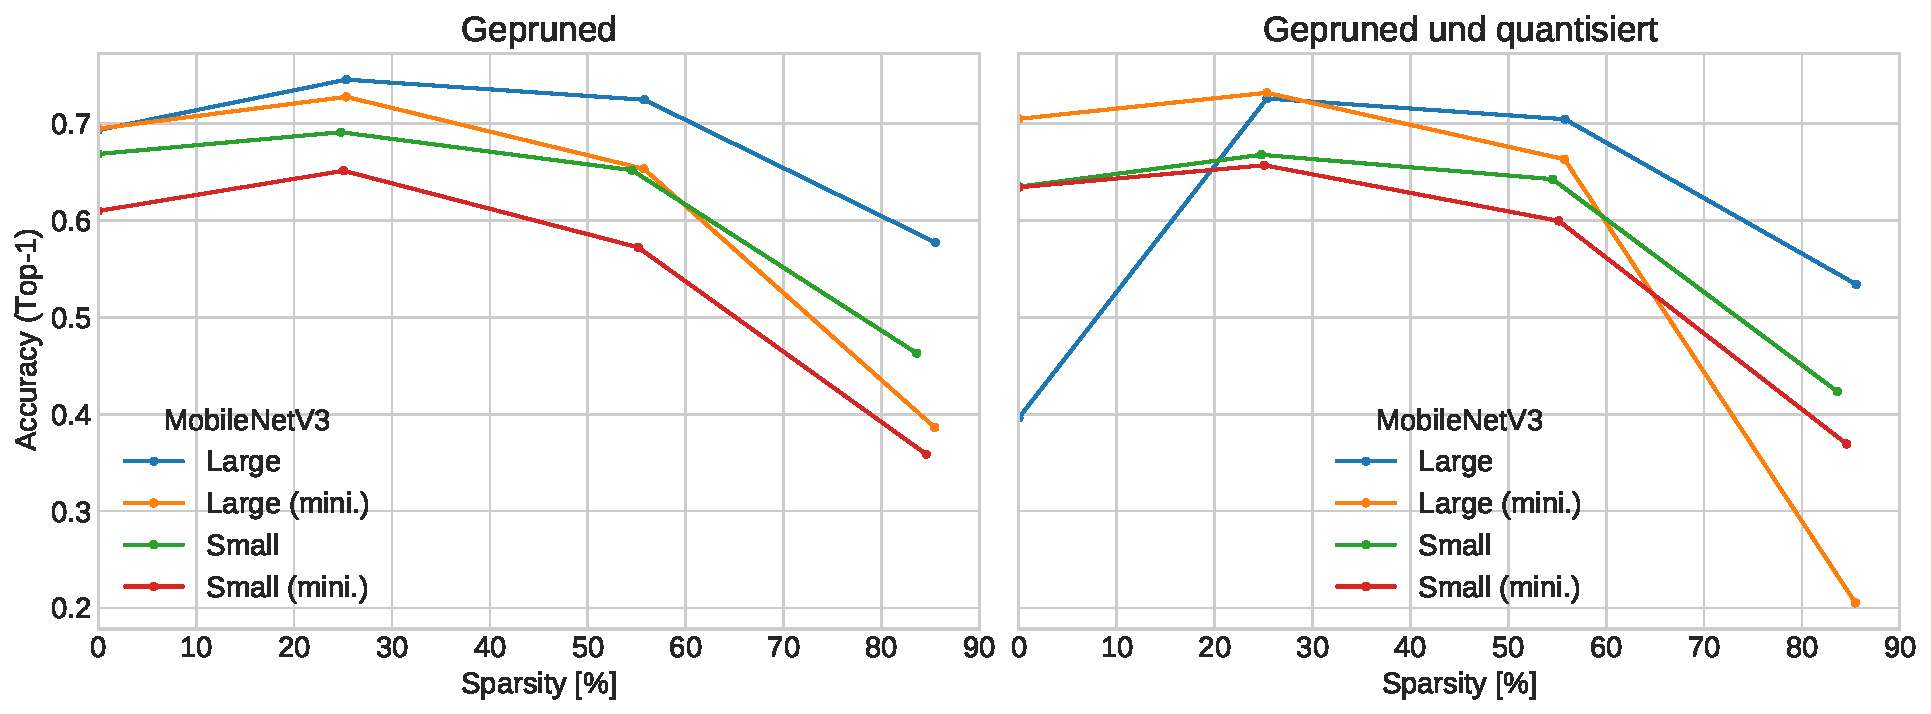
\includegraphics[width=\textwidth]{content/images/sparsity_vs_accuracy_mnv3mini.pdf}}
\caption{Genauigkeiten (Top-1) der MobileNetV3 Architekturen auf den Testdaten für die tatsächlichen Sparsity-Werte beim Pruning auf $0\%$ (ungepruned), $30\%$, $60\%$ und $90\%$ Sparsity und auf der linken Seite nach anschließender Post-Training Quantisierung dieser Modelle.}
\label{f4.10}
\end{figure}

Es lässt sich in Abschnitt \ref{eval_pruning} erkennen, dass auch die MobileNetV3 Minimalistic Modelle mit zunehmender Sparsity an Genauigkeit verlieren. Zusätzlich lässt sich erkennen, dass der Verlust an Genauigkeit bei den Minimalistic-Varianten mit zunehmender Sparsity etwas stärker ausfällt als bei den normalen MobileNetV3 Modellen. Bei dem quantisierten MobileNetV3 Large Minimalistic sinkt die Top-1 Genauigkeit auf den Testdaten sogar auf ca. $20\%$ ab, während das einfache MobileNetV3 Large beim Pruning auf $90\%$ Sparsity und anschließender Quantisierung eine Genauigkeit von $53\%$ beibehält. Der Grund dafür, warum die MobileNetV3 Minimalistic Architekturen bei zunehmender Sparsity schlechtere Genauigkeiten erzielen als die normalen MobileNetV3 Architekturen, ist vermutlich, dass die Minimalistic-Varianten von Grund auf schon weniger Parameter besitzen als die normalen MobileNetV3 Architekturen und dadurch stärker auf eine weitere Reduzierung der Parameter reagieren. Außer dem Genauigkeitsverlust ändern sich die anderen Metriken der MobileNetV3 Minimalistic Architekturen aber nicht, wie bereits in Abschnitt \ref{eval_pruning} diskutiert. Abgesehen von der Genauigkeit sind die anderen Metriken der MobileNetV3 Minimalistic Modelle in derselben Größenordnung wie in Tabelle \ref{t4.7} und Tabelle \ref{t4.8} beschrieben.

Werden nun aber die geprunten und geprunten \& quantisierten MobileNetV3 Minimalistic Modelle wie im Abschnitt \ref{eval_pruning} mittels des Kompressionsalgorithmus gzip komprimiert, lässt sich die Größe der einzelnen Architekturen nochmals deutlich reduzieren. Abbildung \ref{f4.11} zeigt die Dateigrößen der komprimierten MobileNetV3 Modelle inklusive der Minimalistic-Varianten für die verschiedenen Sparsity-Werte. Wie auch in Abschnitt \ref{eval_pruning} gesehen, lässt sich die Größe der einzelnen Architekturen mit zunehmender Sparsity immer weiter komprimieren. Damit ist die kleinste betrachtete Architektur in diesem Paper die MobileNetV3 Small Minimalistic Architektur mit ca. 1 Millionen Parametern und einer Dateigröße des nicht quantisierten Modells von 6.2MB. Wird dieses Modell komprimiert, quantisiert und auf $90\%$ Sparsity gepruned, beträgt die Dateigröße nur noch 0.36MB.

\begin{figure}[htbp]
\centerline{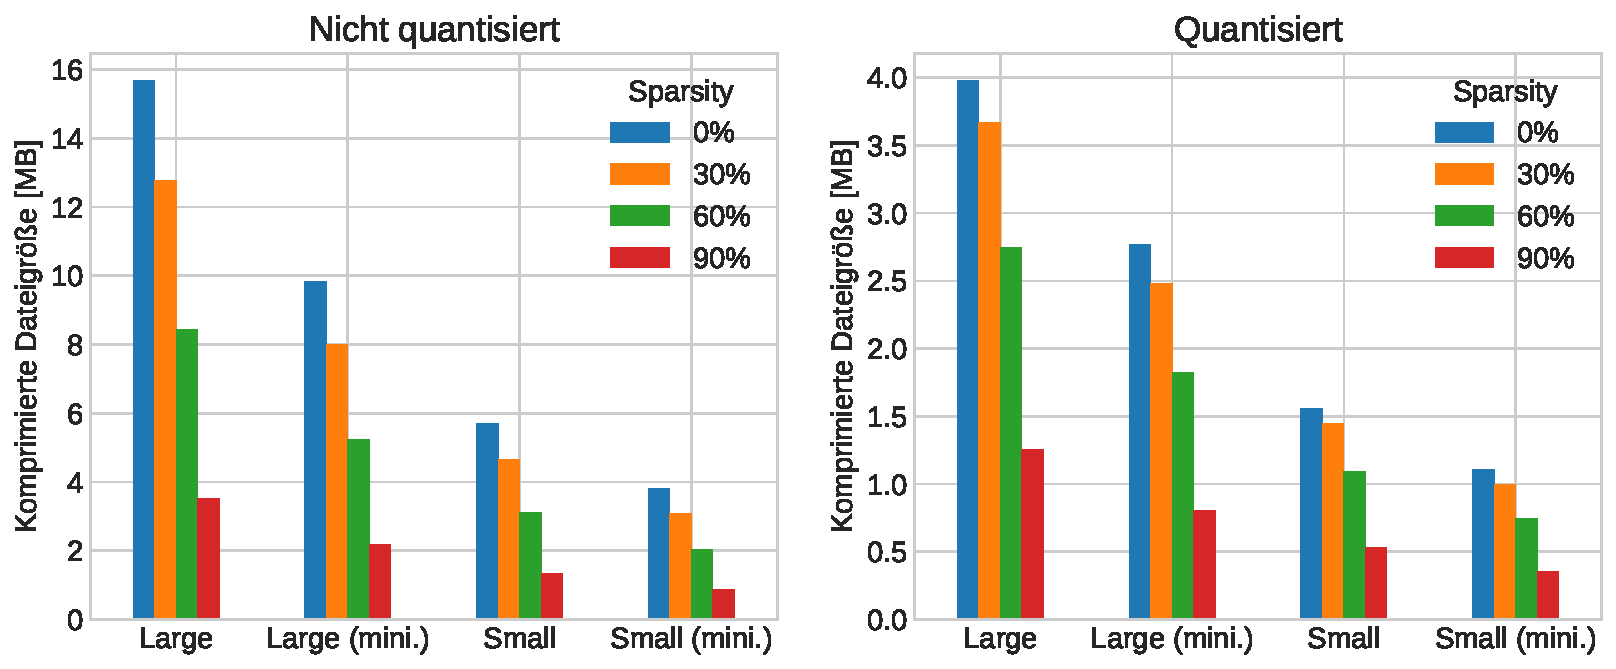
\includegraphics[width=\textwidth]{content/images/pruned_and_compressed_mnv3mini.pdf}}
\caption{Dateigröße für die MobileNetV3 Modelle mit $0\%$, $30\%$, $60\%$ und $90\%$ Sparsity nach Anwendung des gzip Kompressionsalgorithmus.}
\label{f4.11}
\end{figure}

Zusammengefasst haben die Verbesserungen der MobileNetV3 Architektur durch das Entfernen der Squeeze-And-Excitation Module, Austauschen der Hard-Swish Aktivierungsfunktion durch ReLU und die Reduzierung der Kernelgrößen in den Convolution-Schichten folgende Effekte ergeben:
\begin{itemize}
\item Das Entfernen der Squeeze-And-Excitation Module und das Ersetzen von $5 \times 5$ Convolutions durch $3 \times 3$ Convolutions hat die Anzahl an Parametern stark verringert und somit besitzen die Minimalistic-Varianten weniger Parameter und benötigen damit auch weniger Haupt- und Hintergrundspeicher.
\item Durch das Entfernen der Squeeze-And-Excitation Schichten, welche auf dem Rasp\-berry Pi 4 zu einer erhöhten Inferenzzeit geführt haben, konnte die Inferenzzeit auf dem Raspberry Pi 4 reduziert werden.
\item Möglicherweise hat das Austauschen der Hard-Swish Aktivierungsfunktion durch ReLU zu der verbesserten Genauigkeit beim Quantisieren der MobileNetV3 Minimalistic Architekturen im Gegensatz zu den normalen MobileNetV3 Architekturen geführt (siehe Abbildung \ref{f4.9}). Diese Vermutung ist damit begründet, da das Austauschen der Swish Aktivierungsfunktion durch ReLU6 bei den EfficientNet-lite Architekturen ebenfalls zu einer Verbesserung der Genauigkeit bei der Quantisierung geführt hat \cite{liu_higher_2020}.
\end{itemize}



\section{Diskussion}
In der bisherigen Arbeit wurden verschiedene Netzwerkarchitekturen auf dem CIFAR-10 Datensatz trainiert, ggf. mittels Pruning/Quantisierung optimiert und anschließend evaluiert. Bei der Diskussion der Ergebnisse der Evaluation hat sich herausgestellt, dass die einzelnen Architekturen teils sehr unterschiedlich auf die einzelnen Optimierungen reagieren. Den besten Trade-Off zwischen Genauigkeitsverlust und Kompression liefert in dieser Arbeit die MobileNet Architektur. Obwohl die MobileNet Architektur die älteste von den betrachteten Architekturen ist, hat sie, wie bereits in Abschnitt \ref{eval_quantisierung} gesehen, am stärksten von der Post-Training Quantisierung profitiert. Zusätzlich konnte die MobileNet Architektur beim Pruning und bei der Kombination aus Pruning und Quantisierung, mit zunehmender Sparsity, bessere Genauigkeiten erzielen als alle anderen betrachteten Architekturen. Durch die Kombination aus Pruning, Quantisierung und der Anwendung des gzip Kompressionsalgorithmus lässt sich der Speicherbedarf dieser Architektur auf 0.9MB verkleinern. Damit ist das MobileNet, bezogen auf den Hintergrundspeicherbedarf, nach der MobileNetV3 Small und MobileNetV2 Architektur, die drittkleinste Architektur. Wenn die Anwendung viel Wert auf eine hohe Genauigkeit legt und auf ein Pruning verzichtet werden kann, dann bieten sich statt der MobileNet Architektur die MobileNetV2 oder EfficientNet-B0 Architektur an. Die MobileNetV2 und EfficientNet-B0 Architektur haben im nicht-optimierten und quantisierten Zustand eine höhere Genauigkeit als die MobileNet Architektur. Jedoch sobald ein Pruning angewendet werden soll, geht der Genauigkeitsvorteil gegenüber der MobileNet Architektur verloren.

\chapter{Zusammenfassung und Ausblick}
In diesem Kapitel wird diese Bachelorarbeit abgeschlossen und der Inhalt zusammengefasst. Außerdem wird ein Ausblick auf mögliche weiterführende Arbeiten an dieser Arbeit gegeben.



\section{Zusammenfassung}
Die Zielsetzung dieser Arbeit war die Auswirkungen der Optimierungstechniken Quantisierung und Pruning auf Netzwerkarchitekturen speziell für mobile und eingebettete Anwendungsbereiche zu untersuchen. Für diese Untersuchung musste ein geeignetes Evaluationsverfahren entwickelt werden.

Um die Auswirkungen der Optimierungstechniken auf Netzwerkarchitekturen für mobile und eingebettete Systeme zu untersuchen, muss in erster Linie eine Auswahl zu betrachtender Architekturen getroffen werden und dessen architekturellen Besonderheiten beleuchtet werden. In dieser Arbeit wurden in Kapitel \ref{grundlagen} die Architekturen MobileNet, MobileNetV2, MobileNetV3 und das EfficientNet genauer beschrieben. Außerdem wurde in diesem Kapitel auch besprochen, wie das von TensorFlow implementierte Quantisierungsschema funktioniert und was ein Magnitude Pruning bedeutet.

Nachdem die benötigten Grundlagen besprochen wurden, wurde in Kapitel \ref{ansatz_und_implementierung} das Vorgehen genauer beleuchtet, mit dem die Auswirkungen von Quantisierung und Pruning auf die Netzwerkarchitekturen untersucht werden sollten. Außerdem wurde vorgestellt wie Training, Quantisierung und Pruning mittels der Python-Bibliothek TensorFlow auf die verschiedenen Architekturen angewendet worden ist. Dabei wurde besonders auf eine einheitliche Parameterwahl in den Schritten Training, Quantisierung und Pruning geachtet, um die Architekturen zum Schluss besser miteinander vergleichen zu können. Diese einheitliche Parameterwahl hat aber, wie sich später herausgestellt hat, möglicherweise zu einem suboptimalen Training der MobileNetV3 Architekturen geführt. Zusätzlich war es bei den MobileNetV3 und EfficientNet Architekturen nötig einige Schichten vom Pruning auszuschließen, um ein Pruning dieser Architekturen in TensorFlow durchführen zu können.

Nachdem alle Architekturen dem Vorgehen entsprechend trainiert und optimiert wurden, folgte in Kapitel \ref{evaluation} die Evaluation der trainierten Modelle. Dazu wurden zu Beginn 5 Metriken definiert, welche teilweise auf dem Raspberry Pi 4 als exemplarische Plattform für mobile/eingebettete Anwendungen ausgewertet wurden. Die gewählten Metriken waren: Top-1/Top-3 Genauigkeit, Parameterzahl, Bedarf an Hintergrundspeicher, Bedarf an Hauptspeicher und Inferenzzeit. Mittels diesen Metriken sollten die Auswirkungen der Optimierungstechniken Quantisierung und Pruning gemessen werden. Was grundsätzlich nach dem Training der Architekturen aufgefallen ist, war, dass die Squeeze-And-Excitation Module, besonders bei der EfficientNet-B0 Architektur, zu einer deutlich erhöhten Inferenzzeit geführt haben. Zu der Quantisierung lässt sich zusammenfassen, dass eine Post-Training Float Fallback Quantisierung dieser vorgestellten Netzwerkarchitekturen durchaus sehr sinnvoll sein kann, da sie zu einer deutlichen Reduzierung der Modellgröße und sogar in einigen Fällen zu einer Verbesserung der Genauigkeit der quantisierten Modelle führt. Beim Pruning hat sich im Wesentlichen herausgestellt, dass ein Magnitude Pruning mit zunehmender Sparsity häufig die Genauigkeit der Modelle verschlechtert, sonst aber keine direkten Auswirkungen auf die restlichen Metriken hat. Wird jedoch auf die geprunten Modelle ein Kompressionsalgorithmus angewendet, kann die Größe der Modelle durch das Pruning stark reduziert werden. Werden die geprunten Modelle vor der Kompression noch quantisiert, kann die Modellgröße noch weiter reduziert werden. Zusätzlich zu den bis dahin betrachteten Metriken wurde in diesem Kapitel auch noch die klassenweise Genauigkeit als wichtige Metrik vorgestellt, um die ungleichmäßige Auswirkung von Quantisierung und Pruning auf die Genauigkeit der einzelnen Klassen zu untersuchen und exemplarisch an 2 Architekturen demonstriert. Danach wurden noch am Beispiel der MobileNetV3 Minimalistc Architekturen mögliche architekturelle Optimierungen untersucht und diskutiert, um die Inferenzzeiten und Parameterzahl der Architekturen zu minimieren und eine bessere Quantisierbarkeit zu gewährleisten. Zum Schluss wurde noch diskutiert welche Architekturen sich am besten für die Aufgabe der Bildklassifikation auf dem CIFAR-10 Datensatz eignen. Dabei hat sich herausgestellt, dass sich die MobileNet Architektur, trotz ihres Alters, immer noch sehr gut für diese Aufgabe eignet.



\section{Ausblick}
Während der Erstellung dieser Arbeit sind einige Stellen aufgetaucht, welche ein Startpunkt für weiterführende Arbeit sein können und welche in dieser Arbeit nicht näher beleuchtet wurden. In diesem Abschnitt sollen genau diese Startpunkte für weiterführende Arbeit diskutiert werden.

In dieser Arbeit wurde auf das Prinzip gesetzt, alle Architekturen mit denselben Parametern zu trainieren und zu optimieren. Dies sollte für vergleichbare Ergebnisse sorgen. Jedoch hat sich im Verlauf der Arbeit herausgestellt, dass dies problematisch sein kann, da beispielsweise die MobileNetV3 Architektur nach dem Training schlechte Ergebnisse erzielt. Außerdem bricht besonders die Genauigkeit der MobileNetV3 Architektur bei der Quantisierung sehr stark ein, was eine Folge des schlechten Trainings sein kann. Eine weiterführende Arbeit könnte sein von diesem einheitlichen Setup abzuweichen und für alle Architekturen einzeln möglichst optimale Parameter für das Training und die Optimierungen zu finden. Dadurch könnte ein realistischeres Bild von den Auswirkungen der Optimierungstechniken Quantisierung und Pruning auf die vorgestellten Architekturen entstehen.

Eine weitere Sache, die in dieser Arbeit aus zeitlichen Gründen nicht weiter betrachtet wurde, ist das Quantization-Aware Training. TensorFlow bietet dazu in dem TensorFlow Model Optimization Toolkit eine Implementierung \footnote{\url{https://www.tensorflow.org/model_optimization/api_docs/python/tfmot/quantization/keras}} dafür. Es könnte interessant sein wie sich ein Quantization-Aware Training im Gegensatz zu der Post-Training Quantisierung auf die mobilen/eingebetteten Netzwerkarchitekturen auswirkt. 

In Bezug auf Quantisierung wurde in dieser Arbeit ausschließlich die Post-Training Float Fallback Quantisierung betrachtet, bei der alle Gewichte und Aktivierungen in 8 Bit Integer quantisiert werden. Jedoch bleibt bei dieser Methode die Eingabe und Ausgabe in 32 Bit Fließkommazahlen. Damit ist diese Art der Quantisierung ungeeignet für eine reine Integer-Only Hardware. Aus diesem Grund könnte in einer weiterführenden Arbeit die Post-Training Integer-Only Quantisierung genauer betrachtet werden, bei der auch die Eingabe und Ausgabe in 8 Bit Integer erfolgt.

Zusätzlich könnte mehr Arbeit investiert werden, um architekturelle Veränderungen an den vorgestellten Netzwerkarchitekturen vorzunehmen, um die Genauigkeit der quantisierten Modelle zu erhöhen. Dazu gibt es bereits Paper, in denen das gemacht wurde \cite{sheng_quantization-friendly_2018}.

Außerdem wurde in dieser Arbeit lediglich der Ansatz des Magnitude Pruning aus dem Jahr 2017 beschrieben \cite{zhu_prune_2017}. Jedoch gibt es eine Vielzahl weiterer Pruning Methoden \cite{gale_state_2019, mishra_survey_2020, tu_pruning_2020}, die auf die vorgestellten Netzwerkarchitekturen angewendet werden könnten und möglicherweise bessere Ergebnisse erzielen könnten als das Magnitude Pruning.



% Appendix chapters to be put here. They will be enumerated with capital letters 
% if you  did not change the \documentclass options.
\begin{appendix}
%\chapter{Anhang}

\begin{table}[ht]
\centering
\begin{tabular}{llp{1.5cm}lll}
\toprule
Architekturen & Sparsity & Exakte Sparsity & Datei [MB] &  RAM [MB]  & Inferenz [µs]   \\
\midrule
MobileNet & 0\% &           0.00\% &     12.8453 &   16.1016 &          11803 \\
                & 30\% &          25.53\% &     12.8453 &   16.2148 &          11392 \\
                & 60\% &          56.21\% &     12.8453 &   16.1289 &          11594 \\
                & 90\% &          86.18\% &     12.8451 &   16.0625 &          11303 \\
\midrule
MobileNetV2 & 0\% &           0.00\% &      8.9153 &   11.2148 &           4961 \\
                & 30\% &          24.72\% &      8.9153 &   11.2656 &           4972 \\
                & 60\% &          54.41\% &      8.9153 &   11.2891 &           4933 \\
                & 90\% &          83.43\% &      8.9153 &   11.2617 &           4948 \\
\midrule
MobileNetV3 Large & 0\% &           0.00\% &     16.8829 &   20.4141 &           8051 \\
                & 30\% &          25.34\% &     16.8829 &   20.4180 &           7992 \\
                & 60\% &          55.78\% &     16.8829 &   20.3750 &           8098 \\
                & 90\% &          85.53\% &     16.8829 &   20.4727 &           8048 \\
\midrule
MobileNetV3 Small & 0\% &           0.00\% &      6.1536 &    8.5859 &           2954 \\
                & 30\% &          24.77\% &      6.1536 &    8.6211 &           2914 \\
                & 60\% &          54.52\% &      6.1536 &    8.6016 &           2959 \\
                & 90\% &          83.60\% &      6.1536 &    8.5898 &           2913 \\
\midrule
EfficientNet-B0 & 0\% &           0.00\% &     16.0860 &   16.6719 &          12453 \\
                & 30\% &          24.47\% &     16.0860 &   16.6484 &          12225 \\
                & 60\% &          53.86\% &     16.0860 &   16.5273 &          12376 \\
                & 90\% &          82.59\% &     16.0860 &   16.4492 &          12237 \\
\bottomrule
\end{tabular}
\caption{Zusammenfassung der exakten Sparsity, Dateigröße, Hauptspeicherbedarf und Inferenzzeit für die geprunten und unquantisierten Modelle}
\label{tA.1}
\end{table}


%\include{appendix_chapterA}
\end{appendix}
%Ende Anhang

%Bibliography
% We strongly recommend to use bibtex to manage your bibliography. It helps you
% structure your references and helps avoiding missing important data for a correct
% quotation. If you have no other idea jabref (http://jabref.sourceforge.net/)
% might be a good idea (Jave runtime environment needed).
% This style is good to use in german master thesis'. You need to have activated
% \usepackage{bigerm} above.
% For english documents just use apalike.
\bibliographystyle{geralpha}

% to finally announce where your bibliography is stored use
\bibliography{content/references/references}
% it is also possible to have several files separated by comma. 
%Bibliographie Angaben mit \bibliography{}

%!TEX root=../../Vorname_Nachname_Diplomarbeit.tex
%pagenumbering{null}

\ 

%clearpage
\cleardoublepage

\ 


\pagestyle{empty}

\textbf{Versicherung an Eides Statt}\\

Ich versichere an Eides statt durch meine untenstehende Unterschrift,
\begin{itemize}
\item[-] dass ich die vorliegende Arbeit - mit Ausnahme der Anleitung durch die Betreuer - selbstständig ohne fremde Hilfe angefertigt habe und
\item[-] dass ich alle Stellen, die wörtlich oder annähernd wörtlich aus fremden Quellen entnommen sind, entsprechend als Zitate gekennzeichnet habe und
\item[-] dass ich ausschließlich die angegebenen Quellen (Literatur, Internetseiten, sonstige Hilfsmittel) verwendet habe und
\item[-] dass ich alle entsprechenden Angaben nach bestem Wissen und Gewissen vorgenommen habe, dass sie der Wahrheit entsprechen und dass ich nichts verschwiegen habe.
\end{itemize}
Mir ist bekannt, dass eine falsche Versicherung an Eides Statt nach \S 156 und \S 163 Abs. 1 des Strafgesetzbuches mit Freiheitsstrafe oder Geldstrafe bestraft wird.
\vfill
Duisburg, \today\\
$\overline{\parbox{4.8cm}{(Ort, Datum)}} ~~~~~~~~~~~~~~~~~~~~~~~~~~~ \overline{\parbox{7cm}{(Julian Hoever)}}$


\end{document}
%%% Local Variables:
%%% mode: latex
%%% TeX-master: t
%%% End:
